\chapter{基于预测模型的端到端高速导航}
本文的第三章提出了一种基于强化学习的端到端运动控制方法，能够完成在未知封闭赛道中的竞速任务。然而在未知的开放复杂环境中，如何实现点到点的高速导航仍然是一个具有挑战性的问题。因此，本文的第四章将继续研究在未知复杂环境中基于预测模型的端到端高速导航方法。首先，本章将对视觉导航问题进行详细的描述，包括长距离导航规划任务，以及常用的模型预测控制框架，并分析其面临的挑战。然后，本章提出了一种基于视觉预测模型的高速导航控制方法，设计一个深度神经网络来预测未来的环境状态，并将其与基于采样的模型预测控制方法相结合，以实现安全高效的导航控制。本章详细介绍了视觉预测模型的架构设计和训练方法，以及基于视觉预测模型的高速导航控制方法的实现细节。最后，通过仿真与实物实验验证了所提出方法在未知复杂环境中的导航性能，并与其他基线方法进行了对比分析。
\section{视觉导航问题描述}
\subsection{长距离导航规划任务}
长距离导航规划任务是指在一个未知的环境中，机器人需要从起始位置导航到目标位置，并且在导航过程中需要避开障碍物和其他动态环境因素。这个任务通常涉及到环境感知、运动控制等多个方面的挑战。机器人需要能够实时地感知周围环境的变化，并根据当前的环境状态进行动态地控制调整，以确保安全高效地到达目标位置。本文期望使用视觉传感器来感知环境，并在高速运动的情况下实现长距离导航规划任务，这对视觉感知和运动控制提出了更高的要求。

由于环境是未知的，机器人无法事先获得完整的环境地图，因此需要依赖于在线感知和预测来进行导航规划。机器人需要能够从视觉输入中提取有用的信息，例如障碍物的位置、动态环境因素的运动趋势等，并将这些信息用于预测未来的环境状态。这些预测可以帮助机器人更好地规划路径和控制策略，以实现安全高效的导航。因此，长距离视觉导航任务可以被构建为一个部分可观测的马尔可夫决策过程（POMDP）。和第三章中的POMDP不同的是，长距离导航问题有一个明确的目标位置，需要在一个更大的环境中进行导航，这增加了问题的复杂性。POMDP可以形式化地表示为一个元组$(\mathcal{S}, \mathcal{A}, \mathcal{G}, \mathcal{T}, \Omega, \mathcal{O},  \mathcal{R}, \gamma)$。其中$s\in\mathcal{S}$表示环境状态空间；$u\in\mathcal{A}$表示动作空间；$g\in\mathcal{G}\subset \mathbb{R}^2$表示导航地目标位置；$\mathcal{T}: \mathcal{S} \times \mathcal{A} \times \mathcal{S} \rightarrow [0,1]$表示状态转移概率函数，状态转移方程为$s_{t+1} \sim p(\cdot \vert s_t, u_t)$；$o\in\Omega$表示观测空间，包括了一张深度图像$I_t\in\mathbb{R}^{H\times W}$和车辆自身的运动状态$\beta_t\in\mathbb{R}^n$；$\mathcal{O}: \mathcal{S} \times \mathcal{A} \times \Omega \rightarrow [0,1]$表示观测概率函数；$\mathcal{R}: \mathcal{S} \times \mathcal{A} \times \mathcal{G} \rightarrow \mathbb{R}$表示奖励函数，包括高速导航奖励以及避障惩罚；$\gamma\in[0,1]$表示折扣因子。在这个POMDP中，机器人需要根据当前的观测来选择动作，以最大化累积奖励，并最终到达目标位置。具体来说，算法需要学习一个策略$\pi(\cdot \vert o_t, g)$来最大化累积奖励：
\begin{equation}
    \pi = \arg\max_{\pi(\cdot \vert o_t, g)} \mathbb{E}_{s_{t+1} \sim p(\cdot \vert s_t, u_t), u_t \sim \pi(\cdot \vert o_t, g)} \left[ \sum_{t=0}^{T-1} \gamma^t r(s_t, u_t, g) \right]
\end{equation}
其中$T$表示导航任务的最大时间步数。通过学习这个策略，机器人可以在未知复杂环境中实现高速导航，并成功到达目标位置。

\subsection{模型预测控制框架}
\begin{figure}[ht]
    \centering
    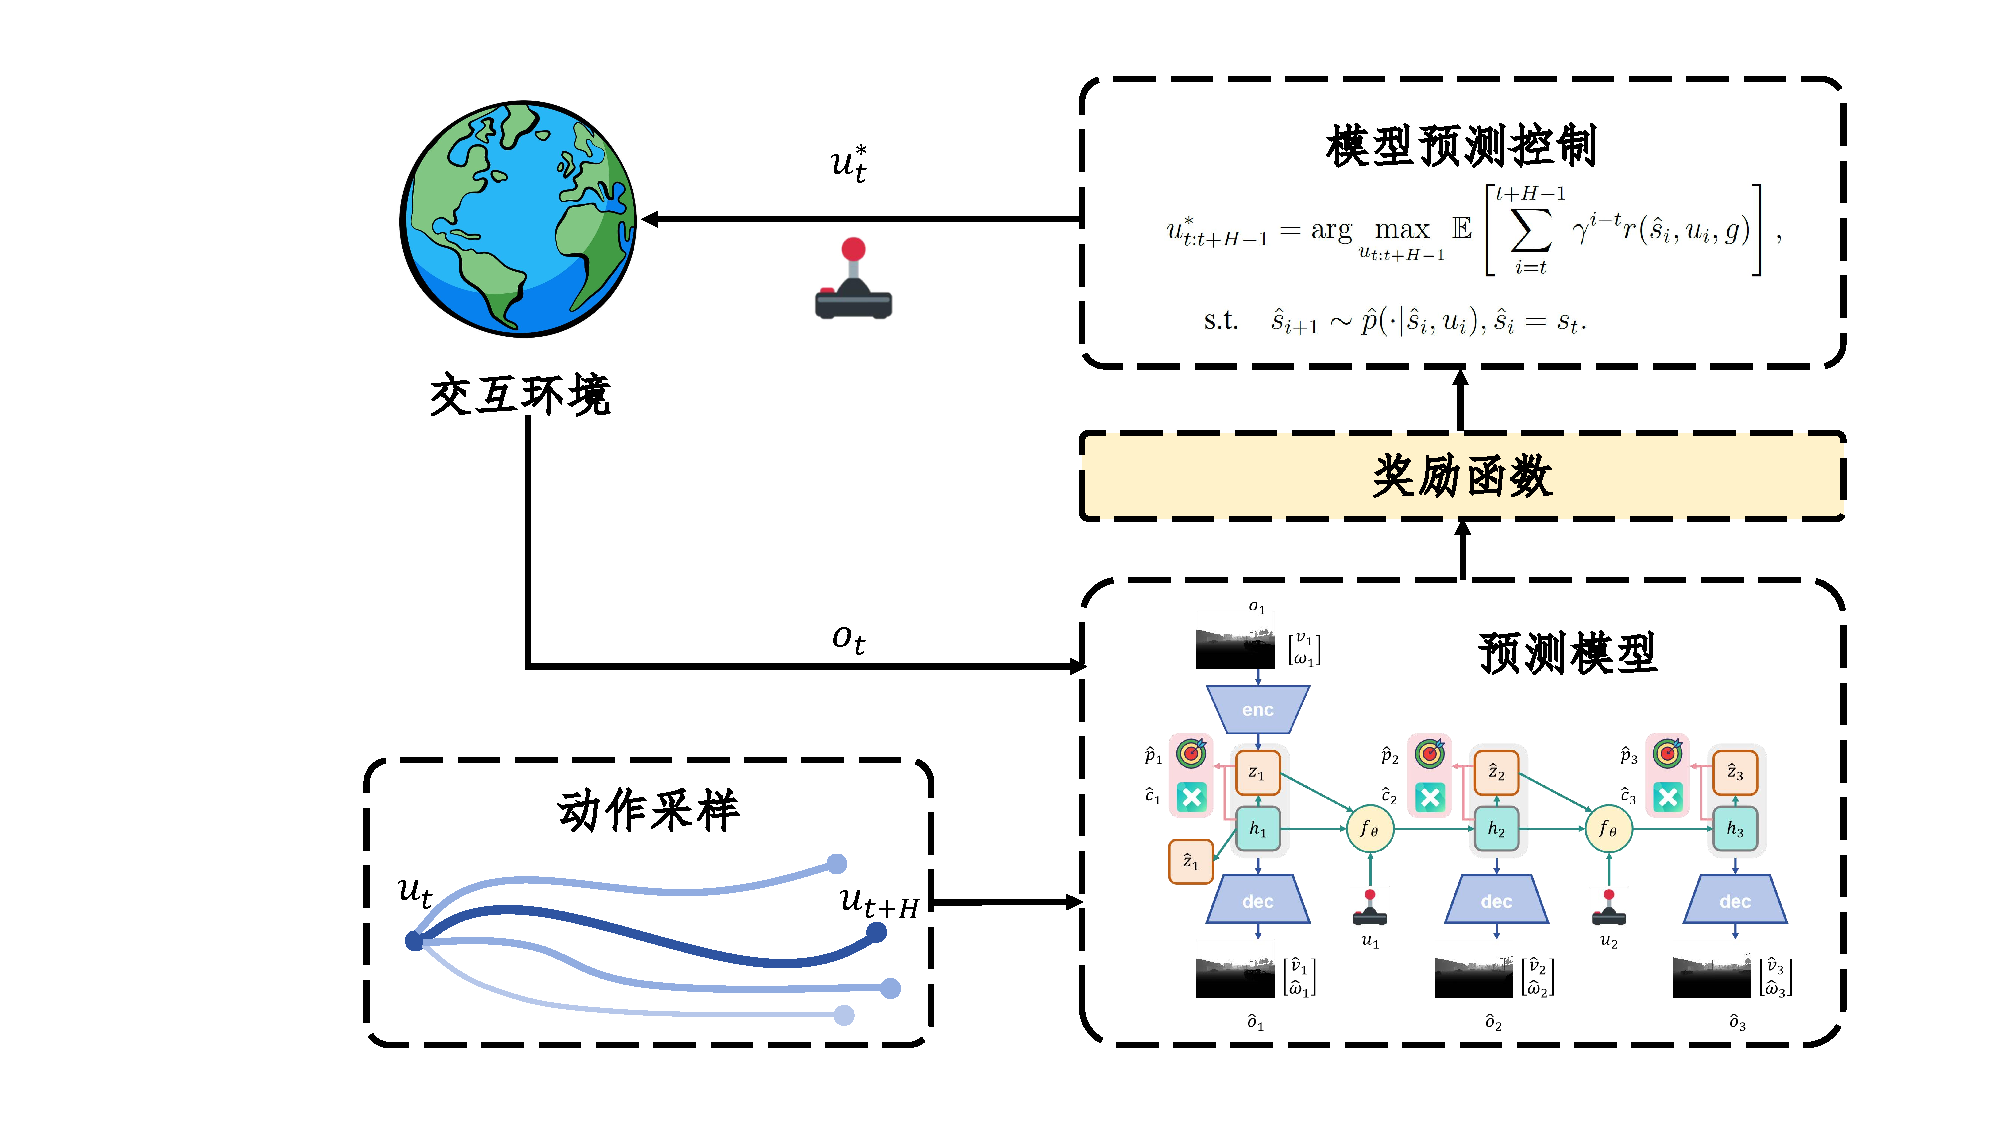
\includegraphics[width=0.8\textwidth]{figure/chapter4/mpc.pdf}
    \caption{模型预测控制框架}
    \label{fig:mpc}
\end{figure}
对于机器人控制问题，现有的研究常用强化学习方法来学习一个直接从观测到动作的策略。然而，在未知复杂环境中，直接学习一个端到端的控制策略可能会面临样本效率低和泛化能力差的问题。在高速导航任务中，机器人需要根据过往的经验来预测未来的环境状态，以便更好地规划路径和控制策略；而强化学习仅能通过与环境的交互来学习一个策略，无法直接利用环境的动态信息进行预测，这导致了策略的短视行为，难以实现长期规划和决策。模型预测控制（MPC）是一种基于模型的控制方法，它通过学习一个环境动态模型来预测未来的环境状态，并利用这些预测来优化控制策略，如图\ref{fig:mpc}所示。MPC方法通过在线优化来选择最优的动作序列，可以实现长序列的动作规划；预测模型能更好地处理未知复杂环境中的不确定性，更具有可解释性。因此，本文将采用基于视觉预测模型的MPC方法来实现未知复杂环境中的高速导航控制。具体来说，MPC在每个时间步$t$都构建了一个轨迹优化问题，来寻找一个最优的动作序列$u_{t:t+H-1} = (u_t, u_{t+1}, \ldots, u_{t+H-1})$，其中$H$表示MPC的预测时域长度。这个优化问题可以形式化地表示为：
\begin{equation}
    \begin{aligned}
        u_{t:t+H-1}^* &= \arg\max_{u_{t:t+H-1}} \mathbb{E}\left[\sum_{i=t}^{t+H-1} \gamma^{i-t} r(\hat{s}_{i}, u_{i}, g) \right] \\
        \text{s.t.} \quad & \hat{s}_{i+1} \sim \hat{p}(\cdot\vert\hat{s}_{i}, u_{i})\\
        & \hat{s}_{i}=s_t\\
        & i=t, \ldots, t+H-1
    \end{aligned}
\end{equation}
% \begin{equation}
%     \begin{aligned}
%         u_{t:t+H-1}^* &= \arg\max_{u_{t:t+H-1}} \mathbb{E}\left[\sum_{i=t}^{t+H-1} \gamma^{i-t} r(\hat{s}_{i}, u_{i}, g) \right], \\
%         \text{s.t.} \quad & \hat{s}_{i+1} \sim \hat{p}(\cdot\vert\hat{s}_{i}, u_{i}),\hat{s}_{i}=s_t.\\
%     \end{aligned}
% \end{equation}
其中$\hat{p}(\cdot\vert\hat{s}_{i}, u_{i})$表示数据驱动方法学习到的环境动态模型，用于预测未来的环境状态$\hat{s}_{i+1}$。求解优化问题得到最优的动作序列$u_{t:t+H-1}^*$后，机器人执行第一个动作$u^*_t$，然后在下一个时间步$t+1$重新构建优化问题，并重复上述过程。因此，由MPC构建的运动策略为$\pi^{\text{MPC}}(o_t, g)=u^*_t$。通过这种方式，MPC方法能够利用环境动态模型的预测能力来实现长期规划和决策，从而在未知复杂环境中实现高速导航控制。

\section{视觉预测模型的设计与训练}\label{sec:model}
\subsection{视觉预测模型架构}
预测模型是MPC方法的核心组件，它负责根据当前的环境状态$s_t$和给定的动作序列$u_{t:t+H-1}$来预测未来的环境状态$\hat{s}_{t+1:t+H}$。然而，由于环境的部分可观性，机器人无法得知完整的状态真值$s_t$，因此需要通过历史观测来推断状态信息。经典的状态空间模型（State Space Model，简称SSM）引入一个隐状态$z_t$来捕捉环境的信息，用状态转移模型$z_{t+1}\sim p(z_{t+1}\vert z_t, u_t)$描述系统随时间的演变，并通过一个观测模型$o_t\sim p(o_t\vert z_t)$将隐状态映射到观测空间。然而，单个随机状态$z_t$往往不够稳定地捕捉环境的动态信息，并且图像这样的高维数据难以直接处理。因此，循环状态空间模型（Recurrent State Space Model，简称RSSM）\cite{hafner2019learning, hafner2020mastering, hafner2023mastering}引入了一个确定性隐藏状态$h_t$，将其与随机状态$z_t$结合起来用于估计环境状态。前者负责处理环境的时序信息，后者负责表示当前时刻的不确定性和随机变化。RSSM能够更好地处理部分可观测环境中的动力学特征，在高速导航任务中具有更好的性能。具体来说，RSSM主要分为以下几个模块：
\begin{equation}
    \begin{aligned}
        &\text{确定性状态转移模型：} & & h_{t+1} = f_{\theta}(h_t, z_{t+1}, u_t) \\
        &\text{随机性状态预测模型：} & & z_t \sim p_{\theta}(z_t\vert h_t)\\
        &\text{观测重建模型：} & & o_t \sim p_{\theta}(o_t\vert z_t, h_t)\\
        &\text{状态预测模型：} & & x_t \sim p_{\theta}(x_t\vert z_t, h_t)
    \end{aligned}
\end{equation}
其中，$\theta$表示模型的参数，确定性状态转移模型$f_{\theta}$用于计算下一个确定性状态$h_{t+1}$，一般由循环神经网络（RNN）实现；随机性状态预测模型$p_{\theta}(z_t\vert h_t)$用于根据当前的确定性状态$h_t$来预测随机状态$z_t$；观测重建模型$p_{\theta}(o_t\vert z_t, h_t)$用于根据当前的状态$z_t$和$h_t$来重建观测$o_t$；状态预测模型$p_{\theta}(x_t\vert z_t, h_t)$用于根据当前的状态$z_t$和$h_t$来预测环境状态$x_t$。
\begin{figure}[ht]
    \centering
    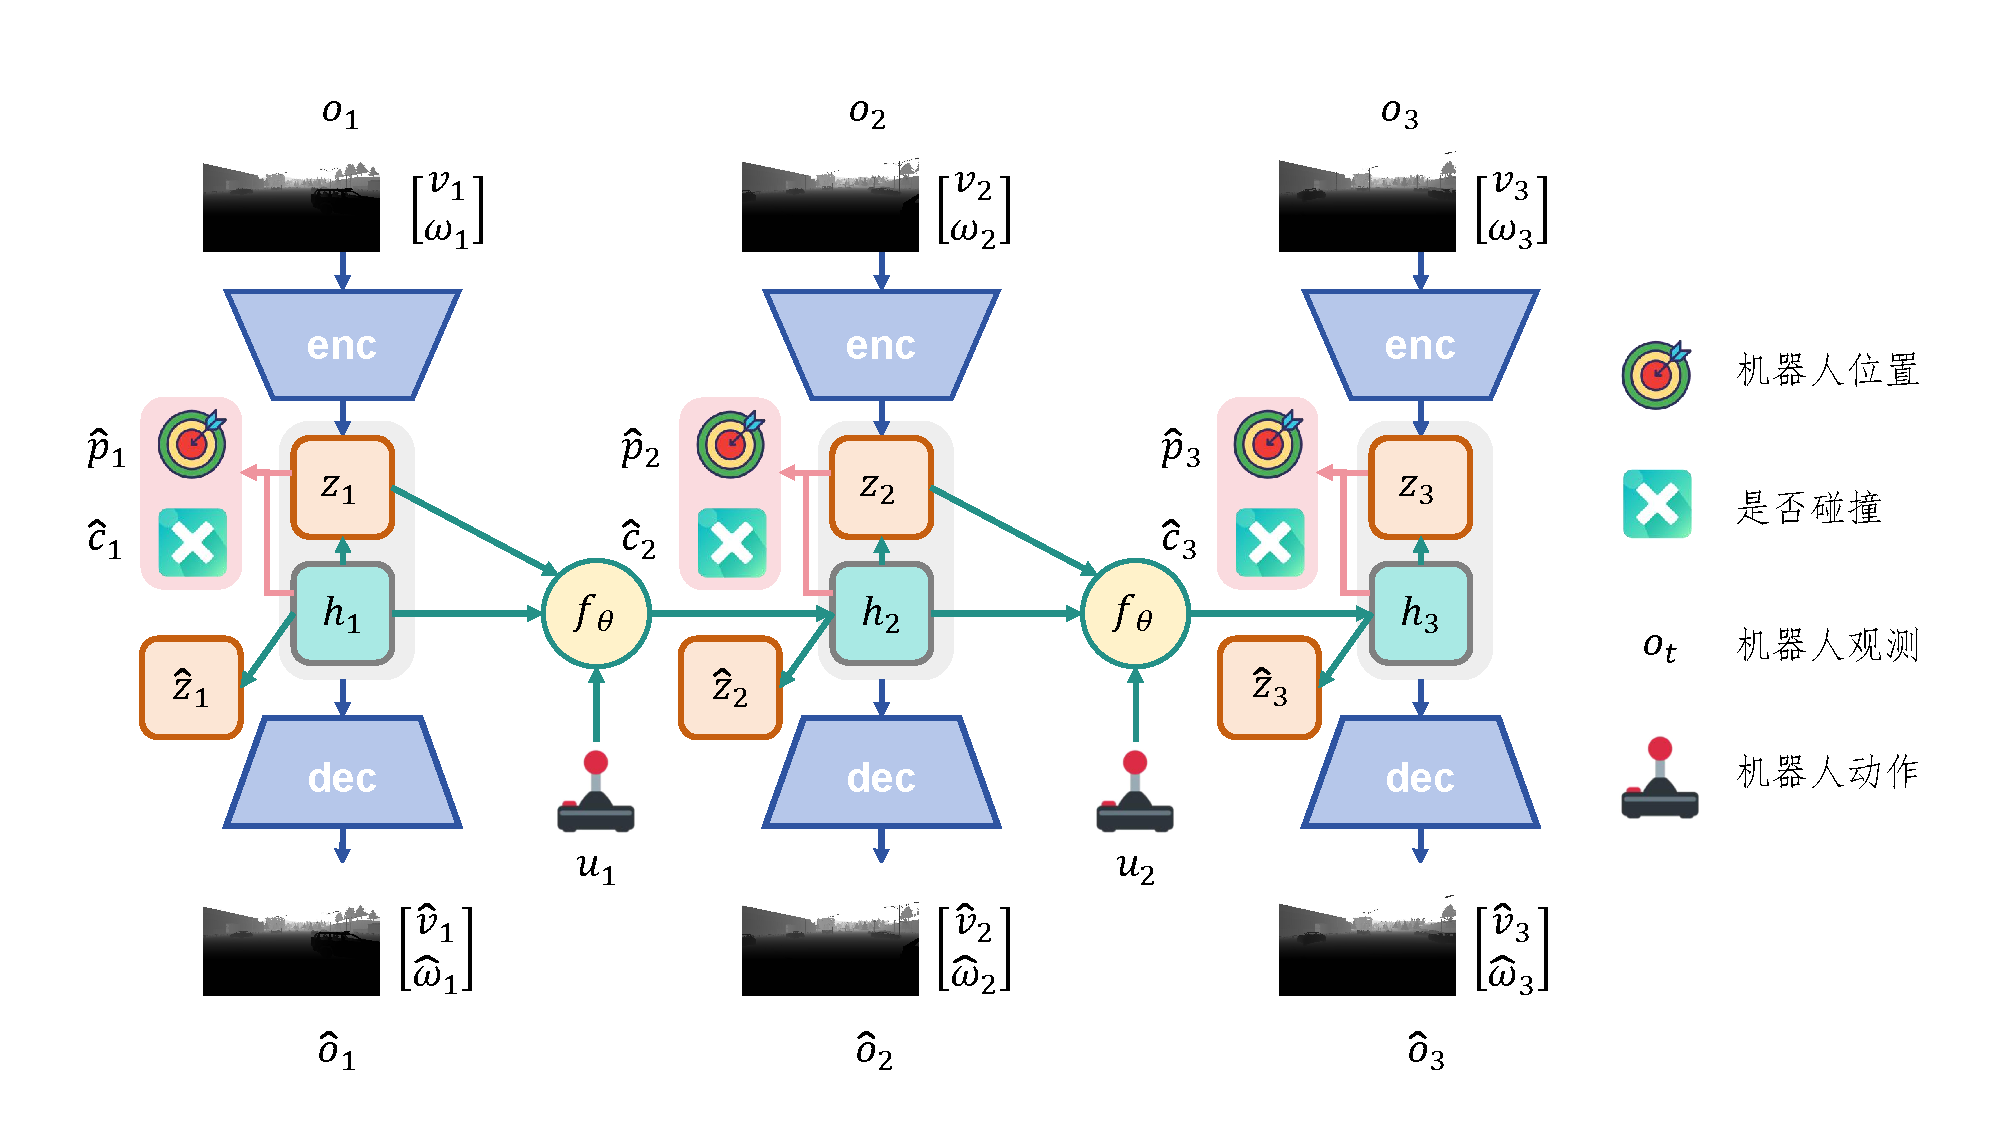
\includegraphics[width=0.9\textwidth]{figure/chapter4/predictive-model.pdf}
    \caption{视觉预测模型整体框架}
    \label{fig:predictive-model}
\end{figure}

图\ref{fig:predictive-model}展示了本文中视觉预测模型（Visual Predictive Model，简称VPM）的整体框架，其中当前观测$o_t$包括深度图像$I_t$和运动状态$\beta_t=[v_t, \omega_t]$，$v_t$表示线速度，$\omega_t$表示角速度，未来环境状态$x_t$包括机器人的位置$p_t$以及碰撞检测$c_t$。$o_t$通过一个编码器$q_{\theta}(z_t\vert o_t)$编码为潜在状态$z_t$，通过一个解码器实现重建模型$p_{\theta}(o_t\vert z_t, h_t)$。同时，$z_t$和$h_t$通过一个前馈网络实现状态预测模型$p_{\theta}(x_t\vert z_t, h_t)$来预测未来环境状态$x_t$。

直观上RSSM的训练应该建立在最大似然估计的基础上，来最大化观测重建模型和状态预测模型的似然函数。然而，由于引入了随机变量$z_t$，直接优化这个目标函数是不可行的。变分推断（Variational Inference）提供了一种有效的优化方法，通过引入一个先验分布来近似后验分布，并通过最大化证据下界（Evidence Lower Bound，简称ELBO）来优化模型参数$\theta$。下面将详细介绍VPM的训练方法，包括ELBO的定义和优化过程，以及如何利用变分推断来训练模型参数$\theta$。
\subsection{视觉预测模型训练方法}
\textbf{模型损失函数：}设一个长度为$T$的轨迹由观测序列$o_{1:T}=(o_1, o_2, \ldots, o_T)$和动作序列$u_{1:T-1}=(u_1, u_2, \ldots, u_{T-1})$，以及潜在变量序列$z_{1:T}=(z_1, z_2, \ldots, z_T)$和状态序列$x_{1:T}=(x_1, x_2, \ldots, x_T)$组成。RSSM的预测过程通常定义如下：首先确定性隐藏状态由递归更新获得：$h_{t+1} = f_{\theta}(h_t, z_{t+1}, u_t)$，其次随机状态由先验分布预测获得：$z_t \sim p_{\theta}(z_t\vert h_t)$，最后观测重建、状态预测由解码器获得：$o_t \sim p_{\theta}(o_t\vert z_t, h_t)$，$x_t \sim p_{\theta}(x_t\vert z_t, h_t)$。于是，给定动作序列$u_{1:T-1}$，RSSM的联合生成分布可以表示为：
\begin{equation}
    \begin{aligned}
    p_{\theta}(o_{1:T}, z_{1:T}, x_{1:T}\vert u_{1:T-1}) = \prod_{t=1}^T p_{\theta}(o_t\vert z_t, h_t) p_{\theta}(z_t\vert h_t) p_{\theta}(x_t\vert z_t, h_t)
    \end{aligned}\label{equ:likelihood}
\end{equation}
训练模型的自然目标是最大化观测数据的边际似然函数：
\begin{equation}
\begin{aligned}
    \mathcal{L}(\theta) = \log p_{\theta}(o_{1:T}, x_{1:T}\vert u_{1:T-1}) = \log \int p_{\theta}(o_{1:T}, z_{1:T}, x_{1:T}\vert u_{1:T-1}) dz_{1:T}
\end{aligned}
\end{equation}
由于直接优化这个目标函数是不可行的，本文引入一个变分分布：
\begin{equation}
\begin{aligned}
    q_{\theta}(z_{1:T}\vert o_{1:T}, u_{1:T-1})=\prod_{t=1}^T q_{\theta}(z_t\vert o_t, h_t)
\end{aligned}\label{equ:post-variance}
\end{equation}
来近似后验分布$p_{\theta}(z_{1:T}\vert o_{1:T}, u_{1:T-1})$，并通过最大化证据下界（ELBO）来优化模型参数$\theta$。首先边际似然函数可以通过引入变分分布来重写为：
\begin{equation}
\begin{aligned}
    \log p_{\theta}(o_{1:T}, x_{1:T}\vert u_{1:T-1}) &= \log \int q_{\theta}(z_{1:T}\vert o_{1:T}, u_{1:T-1}) \frac{p_{\theta}(o_{1:T}, z_{1:T}, x_{1:T}\vert u_{1:T-1})}{q_{\theta}(z_{1:T}\vert o_{1:T}, u_{1:T-1})} dz_{1:T} \\
    &= \log \mathbb{E}_{q_{\theta}(z_{1:T}\vert o_{1:T}, u_{1:T-1})} \left[ \frac{p_{\theta}(o_{1:T}, z_{1:T}, x_{1:T}\vert u_{1:T-1})}{q_{\theta}(z_{1:T}\vert o_{1:T}, u_{1:T-1})} \right]
\end{aligned}
\end{equation}
根据琴生不等式（Jensen's Inequality），因为对数函数是凹函数，所以可以得到$\log \mathbb{E}[X] \geq \mathbb{E}[\log X]$，并将公式（\ref{equ:likelihood}、\ref{equ:post-variance}）代入，从而得到证据下界（ELBO）：
\begin{equation}
\begin{aligned}
    \log p_{\theta}(o_{1:T}, x_{1:T}\vert u_{1:T-1}) &\geq \mathbb{E}_{q_{\theta}(z_{1:T}\vert o_{1:T}, u_{1:T-1})} \left[ \log \frac{p_{\theta}(o_{1:T}, z_{1:T}, x_{1:T}\vert u_{1:T-1})}{q_{\theta}(z_{1:T}\vert o_{1:T}, u_{1:T-1})} \right] \\
    & = \mathbb{E}_{q_{\theta}(z_{1:T}\vert o_{1:T}, u_{1:T-1})} \left[ \log \frac{\prod_{t=1}^T p_{\theta}(o_t\vert z_t, h_t) p_{\theta}(z_t\vert h_t) p_{\theta}(x_t\vert z_t, h_t)}{\prod_{t=1}^T q_{\theta}(z_t\vert o_t, h_t)} \right] \\
    & \triangleq \mathcal{L}_{\text{ELBO}}(\theta)
\end{aligned}
\end{equation}
利用对数函数的性质，连乘积可以转化为求和，因此ELBO可以进一步展开为：
\begin{equation}
\begin{aligned}
    \mathcal{L}_{\text{ELBO}}(\theta) &= \sum_{t=1}^T \mathbb{E}_{q_{\theta}(z_t\vert o_t, h_t)} \left[ \log p_{\theta}(o_t\vert z_t, h_t) + \log p_{\theta}(z_t\vert h_t) + \log p_{\theta}(x_t\vert z_t, h_t) - \log q_{\theta}(z_t\vert o_t, h_t) \right] \\
    &= \sum_{t=1}^T \mathbb{E}_{q_{\theta}(z_t\vert o_t, h_t)} \left[ \log p_{\theta}(o_t\vert z_t, h_t) + \log p_{\theta}(x_t\vert z_t, h_t) \right] - \sum_{t=1}^T \mathbb{E}_{q_{\theta}(z_t\vert o_t, h_t)} \left[ \log \frac{q_{\theta}(z_t\vert o_t, h_t)}{p_{\theta}(z_t\vert h_t)} \right]
\end{aligned}
\end{equation}
为了直观和优化的方便，可以将ELBO的第二项表示为Kullback-Leibler (KL) 散度的形式，其定义为$D_{KL}(P\Vert Q) = \mathbb{E}_{P}[\log \frac{P}{Q}]$，因此ELBO可以最终表示为：
\begin{equation}
\begin{aligned}
    \mathcal{L}_{\text{ELBO}}(\theta) = \sum_{t=1}^T \mathbb{E}_{q_{\theta}(z_t\vert o_t, h_t)} \left[ \log p_{\theta}(o_t\vert z_t, h_t) + \log p_{\theta}(x_t\vert z_t, h_t) \right] - \sum_{t=1}^T D_{KL} \left(q_{\theta}(z_t\vert o_t, h_t) \Vert p_{\theta}(z_t\vert h_t)\right)
\end{aligned}
\end{equation}
其中第一项表示未来观测和状态预测的重建误差，要求模型能从当前潜在状态$(h_t, z_t)$中准确还原观测和状态；第二项表示后验分布与先验分布之间的KL散度，鼓励先验分布接近后验分布。在想象阶段（无需真实环境观测），机器人只能依靠先验分布来推进潜状态。如果这一项被优化得很小，说明转移模型仅仅通过历史信息就能准确预测出未来状态的概率分布，从而使得在潜空间中的开环预测（Open-loop prediction）变得可靠。一般在实际的训练过程中，研究者会使用两个KL散度来强制要求潜在空间保持一致且不发生坍缩\cite{chen2021exploring}。最终的优化目标可以表示为：
\begin{equation}
\begin{aligned}
    \mathcal{L}_{\text{ELBO}}(\theta) =& \sum_{t=1}^T [ \mathcal{L}_{\text{recon}}(\theta) -\mathcal{L}_{\text{KL}}(\theta) ] \\
    \mathcal{L}_{\text{recon}}(\theta) =& \mathbb{E}_{z_t\sim q_{\theta}(z_t\vert o_t, h_t)} [\log p_{\theta}(o_t\vert z_t, h_t) + \log p_{\theta}(x_t\vert z_t, h_t)] \\
    \mathcal{L}_{\text{KL}}(\theta) =& D_{KL}\left(\text{sg}(q_{\theta}(z_t\vert o_t, h_t)) \Vert p_{\theta}(z_t\vert h_t)\right) +\\
    & D_{KL}\left(q_{\theta}(z_t\vert o_t, h_t) \Vert \text{sg}(p_{\theta}(z_t\vert h_t))\right)
\end{aligned}
\end{equation}

由于$z_t$是从依赖于模型参数$\theta$的分布中采样的，而采样是一个随机、不可微的操作，因此ELBO的优化目标无法直接使用梯度下降等优化方法来更新模型参数$\theta$。为了能够使优化目标反向传播到模型参数$\theta$，本文使用重参数化技巧（Reparameterization Trick）来对随机变量$z_t$进行采样。其核心思想是：将随机性与参数解耦，把原本带有参数的随机变量，转化为一个确定性的参数化函数与一个无参数的随机变量的组合。首先，假设后验分布$q_{\theta}(z_t\vert o_t, h_t)$是对角协方差的高斯分布，即$q_{\theta}(z_t\vert o_t, h_t) = \mathcal{N}(\mu_{q}(o_t, h_t), \sigma^2_{q}(o_t, h_t))$。然后可以通过以下方式来进行重参数化采样：
\begin{equation}
\begin{aligned}
    z_t &= \mu_{q}(o_t, h_t) + \sigma_{q}(o_t, h_t) \odot \epsilon \\
    \epsilon &\sim \mathcal{N}(0, I)
\end{aligned}
\label{equ:reparameterization}
\end{equation}
其中$\epsilon$是一个从标准正态分布中采样的随机变量，$\odot$表示元素级乘法。通过这种方式，随机采样操作被转移到无参数的$\epsilon$上，而模型参数$\theta$只影响确定性的函数$\mu_{q}(o_t, h_t)$和$\sigma_{q}(o_t, h_t)$，从而使得$\mathcal{L}_{\text{recon}}$的梯度可以直接移到内部的函数上进行优化：
\begin{equation}
\begin{aligned}
    \nabla_{\theta} \mathcal{L}_{\text{recon}}(\theta) &= \mathbb{E}_{\epsilon \sim \mathcal{N}(0, I)} \left[ \nabla_{\theta} \log p_{\theta}(o_t\vert z_t, h_t) + \nabla_{\theta} \log p_{\theta}(x_t\vert z_t, h_t) \right]\\
    &= \mathbb{E}_{\epsilon \sim \mathcal{N}(0, I)} \left[-\nabla_{\theta} \frac{\Vert o_t - \mu_o(z_t, h_t) \Vert^2}{2 \sigma_o^2(z_t, h_t)} - \nabla_{\theta}  \frac{\Vert x_t - \mu_x(z_t, h_t) \Vert^2}{2 \sigma_x^2(z_t, h_t)} \right]
\end{aligned}
\end{equation}
其中$\mu_o(z_t, h_t)$和$\sigma_o^2(z_t, h_t)$分别表示观测重建模型$p_{\theta}(o_t\vert z_t, h_t)$的均值和方差；$\mu_x(z_t, h_t)$和$\sigma_x^2(z_t, h_t)$分别表示状态预测模型$p_{\theta}(x_t\vert z_t, h_t)$的均值和方差，$z_t$由公式（\ref{equ:reparameterization}）进行重参数化采样得到。

\newpage
运用重参数化技巧后，我们无法穷举正态分布中的所有可能的$\epsilon$，因此通常会使用蒙特卡洛方法来近似计算期望值，即通过多次采样$\epsilon$来估计梯度的期望。在实际训练中，为了保证计算效率，通常在每个时间步只采样一次，即样本数$L=1$。对于KL散度项的优化，可以使用封闭形式的KL散度计算方法来直接计算正态分布KL散度的值，而不需要进行采样估计：
\begin{equation}
\begin{aligned}
    D_{KL}\left(q_{\theta}(z_t\vert o_t, h_t) \Vert p_{\theta}(z_t\vert h_t)\right) =& \frac{1}{2} \sum_{i=1}^d \left[ 2\log\frac{\sigma_{p,i}}{\sigma_{q,i}} + \frac{\sigma^2_{q,i}+(\mu_{p,i} - \mu_{q,i})^2}{\sigma^2_{p,i}} - 1 \right]
\end{aligned}
\end{equation}
其中$d$表示潜在空间的维度，$\mu_{p,i}$和$\sigma_{p,i}$分别表示先验分布$p_{\theta}(z_t\vert h_t)$的第$i$维的均值和标准差；$\mu_{q,i}$和$\sigma_{q,i}$分别表示后验分布$q_{\theta}(z_t\vert o_t, h_t)$的第$i$维的均值和标准差。

综上，RSSM能在神经网络中反向传播的损失函数可以表示为：
\begin{equation}
\begin{aligned}
    \mathcal{J}_{\text{RSSM}}(\theta) =& \mathbb{E}_{\tau\sim\mathcal{D}} \sum_{t=1}^T [\mathcal{J}_{\text{recon}}(\theta) + \mathcal{J}_{\text{KL}}(\theta)] \\
    \mathcal{J}_{\text{recon}}(\theta) =& \frac{\Vert o_t - \mu_o(z_t, h_t) \Vert^2}{2 \sigma_o^2(z_t, h_t)}  + \frac{\Vert x_t - \mu_x(z_t, h_t) \Vert^2}{2 \sigma_x^2(z_t, h_t)} \\
    \mathcal{J}_{\text{KL}}(\theta) =& D_{KL}\left(\text{sg}(q_{\theta}(z_t\vert o_t, h_t)) \Vert p_{\theta}(z_t\vert h_t)\right) + \\
    & D_{KL}\left(q_{\theta}(z_t\vert o_t, h_t) \Vert \text{sg}(p_{\theta}(z_t\vert h_t))\right)
\end{aligned}
\end{equation}
其中$\tau\sim\mathcal{D}$表示从经验回放缓冲区$\mathcal{D}$中采样一个轨迹$\tau$，在每个时间步$t$上计算重建误差和KL散度的损失函数。模型参数$\theta$通过最小化这个损失函数来进行优化，从而使得VPM能够更好地捕捉环境的动态特征：
\begin{equation}
\begin{aligned}
    \theta^* = \arg\min_{\theta} \mathcal{J}_{\text{RSSM}}(\theta)
\end{aligned}
\end{equation}

\textbf{数据收集与模型推理：}VPM的训练数据通常来自于机器人与环境的交互过程中收集的轨迹数据。数据收集的原则是大量探索状态和动作空间，使其尽可能地覆盖环境的动态特征和不确定性。这些数据可以通过随机策略、预训练的控制策略或者人类示范等方式在仿真环境或现实环境中收集。在仿真中，可以通过随机策略或预训练的策略来收集数据，即在每个时间步$t$随机选择一个动作$u_t$来与环境进行交互，并记录下观测$o_t$、动作$u_t$以及环境状态$x_t$等信息。虽然仿真环境只提供了一个简化的环境模型，但它能够提供大量的交互数据来训练VPM。在现实环境中，可以通过人类示范来收集数据。虽然现实环境中的数据收集可能会受到安全性和效率的限制，但它能够提供更真实的环境交互数据来微调VPM，从而提高模型在现实环境中的性能和泛化能力。

为了减少数据收集的成本和风险，本文采用一种混合的数据收集策略，即先在仿真环境中收集大量的交互数据来预训练VPM，然后在现实环境中通过人类示范收集轨迹数据来进一步微调模型参数。具体来说，首先采用了第二章提出的参数辨识方法（System Identification, 简称SysID）来学习一个动力学模型，并在仿真中设置相应的参数来最大化仿真与现实的相似性。然后，再采用第三章提出的域随机化技术（Domain Randomization, 简称DR）来进行图像、动力学的数据增强，以增加模型的鲁棒性和泛化能力。接着，在数据增强后的仿真环境中进行预训练，总共分为两个阶段：在第一阶段预训练数据收集过程中，本节采用了一种时间相关的随机采样方式来采样交互动作得到轨迹数据。具体来说，在每个时间步$t$，动作采样的概率分布是一个时间相关的分布，它依赖于上一个时间步$t-1$的动作$u_{t-1}$：
\begin{equation}
\begin{aligned}
    \beta \sim \mathcal{U}(\beta_{\text{min}}, 1)  &\quad u_{\text{rand}} \sim \mathcal{U}(u_{\text{min}}, u_{\text{max}}) \\
    u_t = \beta \cdot  u_{t-1} & + (1-\beta) \cdot u_{\text{rand}}
\end{aligned}
\end{equation}
在第二阶段预训练数据收集过程中，预训练的模型已经有了一定的预测能力，为了防止模型过拟合于时间相关动作采样策略，本文采用基于采样的模型预测控制策略（于本章4.3.1节介绍）来采样动作，并继续收集数据训练。在这样的预训练下，模型能够更好地适应MPC的动作采样方式，从而提高模型在实际控制中的性能和泛化能力。预训练之后，机器人在现实环境中通过人类示范策略采样动作，继续收集数据。与仿真环境中的数据不同，现实环境中的数据主要来源于传感器的状态估计，其中$p_t, v_t$由一个视觉里程计算法估计，$\omega_t$由IMU数据进行滤波估计，$c_t$由人类手动标注，$u_t$由人类示范策略得到。现实环境中的数据收集完成后，与仿真环境中的数据进行合并，并采样更小的学习率来微调模型参数$\theta$。每条轨迹都包含了观测序列$o_{1:T}$，动作序列$u_{1:T}$以及状态序列$x_{1:T}$，这些数据被存储在一个经验回放缓冲区$\mathcal{D}$中，$\mathcal{D}$的数据在更新和采样训练两个阶段交替进行，如算法\ref{algo:model-training}所示。

\newpage
\renewcommand{\algorithmicrequire}{ \textbf{输入：}}
\renewcommand{\algorithmicensure}{ \textbf{输出：}}
\renewcommand{\algorithmicreturn}{ \textbf{返回：}}
\begin{algorithm}[H]
    \begin{spacing}{1.25}
	\caption{视觉预测模型训练算法}
    \renewcommand{\arraystretch}{1.25}
	\label{algo:model-training}
	\begin{algorithmic}[1]
        \REQUIRE 预测模型$\hat{p}$，时间相关采样策略$\pi_{\text{rand}}$，基于采样的MPC策略$\pi_{\text{MPC}}$，数据集$\mathcal{D}$，预训练轮数$T_1$、$T_2$，微调轮数$T_{\text{fine}}$，预训练学习率$\alpha_{\text{pre}}$，微调学习率$\alpha_{\text{fine}}$
		\ENSURE 最佳网络参数$\theta$
        \STATE 初始化数据集$\mathcal{D}$和预测模型$\hat{p}$的参数$\theta$
		\FOR{$i=1, 2, \cdots, T_1+T_2$}{
            \IF{$i \leq T_1$}
                \STATE 在仿真环境中使用$\pi_{\text{rand}}$来采样动作，收集轨迹数据$\tau_i = (o_{1:T}, u_{1:T}, x_{1:T})$
            \ELSE
                \STATE 在仿真环境中使用$\pi_{\text{MPC}}$来采样动作，收集轨迹数据$\tau_i = (o_{1:T}, u_{1:T}, x_{1:T})$
            \ENDIF
            \STATE 更新数据集$\mathcal{D} \leftarrow \mathcal{D} \cup \tau_i$
            \STATE 从数据集$\mathcal{D}$中采样一个批次的轨迹数据，并计算损失函数$\mathcal{J}_{\text{RSSM}}(\theta)$
            \STATE 更新模型参数$\theta \leftarrow \theta - \alpha_{\text{pre}} \nabla_{\theta} \mathcal{J}_{\text{RSSM}}(\theta)$
        }
        \ENDFOR
        \FOR{$i=1, 2, \cdots, T_{\text{fine}}$}{
            \STATE 在仿真环境中使用人类示范收集轨迹数据$\tau_i = (o_{1:T}, u_{1:T}, x_{1:T})$
            \STATE 更新数据集$\mathcal{D} \leftarrow \mathcal{D} \cup \tau_i$
            \STATE 从数据集$\mathcal{D}$中采样一个小批次的轨迹数据，并计算损失函数$\mathcal{J}_{\text{RSSM}}(\theta)$
            \STATE 更新模型参数$\theta \leftarrow \theta - \alpha_{\text{fine}} \nabla_{\theta} \mathcal{J}_{\text{RSSM}}(\theta)$
        }
        \ENDFOR
        \RETURN 最佳网络参数$\theta$
	\end{algorithmic}
    \end{spacing}
\end{algorithm}
\begin{figure}[H]
    \centering
    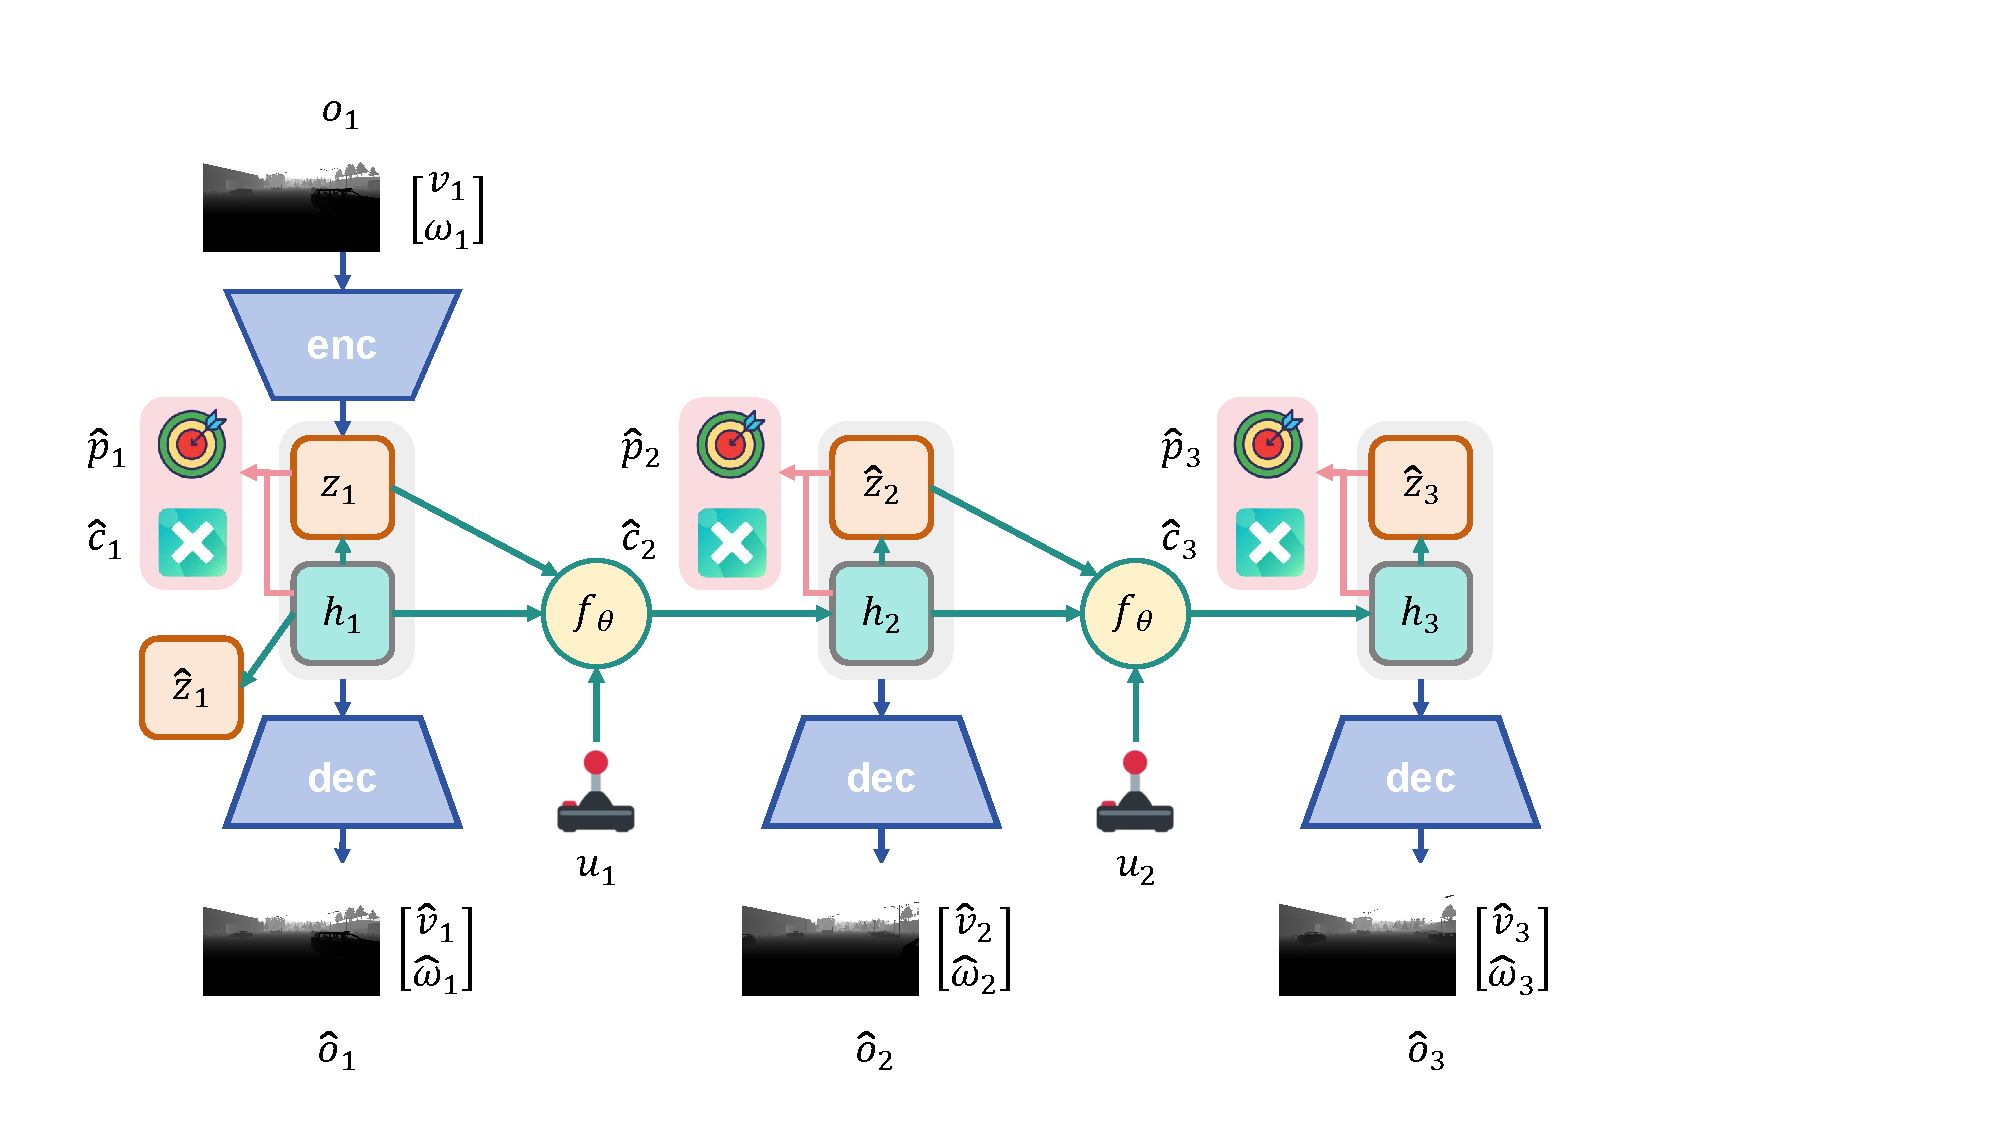
\includegraphics[width=0.75\textwidth]{figure/chapter4/model-inference.pdf}
    \caption{预测模型前向推理}
    \label{fig:model-inference}
\end{figure}

训练完成后，可以使用训练好的VPM来进行前向推理，以预测未来的环境状态。具体来说，在每个时间步$t$，根据当前的观测$o_t$和动作$u_t$来计算潜在状态$z_t$，然后通过确定性状态转移模型$f_{\theta}$来计算下一个确定性状态$h_{t+1}$，最后通过状态预测模型$p_{\theta}(x_{t+1}\vert z_t, h_t)$来预测未来的环境状态$x_{t+1}$。通过不断地迭代这个过程，可以得到一个未来环境状态的预测序列$\hat{x}_{t+1:t+H}$，如图\ref{fig:model-inference}所示。这个预测序列可以被用来评估不同动作序列的长期奖励，从而指导MPC方法来选择最优的动作序列，实现高速导航控制。
\section{基于视觉预测模型的高速导航控制}
\ref{sec:model}节介绍了MPC框架中视觉预测模型的设计与训练方法，接下来本节将介绍如何利用训练好的视觉模型来优化导航控制策略。传统的MPC框架中，模型通常是一个确定性的物理模型或者一个简单的线性模型，优化方法通常是基于梯度的优化方法，如序列二次规划或者连续时间的最优控制方法。然而本文中的模型是一个复杂的神经网络模型，具有非线性和非凸的特性，且状态具有随机性，因此传统的基于梯度的优化方法可能不适用于这个问题。为了应对这个挑战，本文采用了一种基于采样的模型预测路径积分控制方法（Model Predictive Path Integral，简称MPPI）\cite{williams2017information, williams2018information}，即通过在潜在空间中采样不同的动作序列，并利用视觉预测模型来评估这些动作序列的长期奖励，从而选择最优的动作序列来执行。下面将详细介绍MPPI的算法流程以及奖励函数的设计。

\subsection{基于采样的模型预测控制方法}
MPPI采用了随机最优控制与路径积分控制的思路，将最优控制问题转换为一个关于轨迹分布的加权采样问题。具体来说，MPPI首先假设存在一条名义控制序列$U  = (u_0, u_1, \cdots, u_{T-1})$，并围绕它叠加随机扰动。设每个时刻的控制扰动满足高斯分布$\epsilon_t \sim \mathcal{N}(0, \Sigma)$，则实际的控制量为$v_t\sim \mathcal{N}(u_t, \Sigma)$，实际控制序列为$V=(v_0, v_1, \cdots, v_{T-1})$。首先，将\ref{sec:model}节中训练好的VPM表示为：
\begin{equation}
\begin{aligned}
    x_{t+1} = \hat{p}(\cdot\vert x_t, u_t)
\end{aligned}
\end{equation}
通常一条轨迹可记为$\tau=(x_0, v_0, x_1, v_1, \cdots, x_{T-1}, v_{T-1}, x_{T})$，有限时域的累积代价函数定义为：
\begin{equation}
\begin{aligned}
    S(\tau) = \phi(x_{T}) + \sum_{t=0}^{T-1} \left[q(x_{t})+\frac{1}{2}v_t^\top R v_t\right]
\end{aligned}
\end{equation}
其中$q(x_t)$是状态运行代价，$\phi(x_T)$是终端代价，$R$是控制代价矩阵。通过改变$U$，可以改变实际控制序列$V$的分布，从而改变轨迹$\tau$的分布。本文关注三种不同的实际控制序列的分布：（1）定义$\mathbb{P}$为未受控系统中实际控制序列的概率分布，即$U\equiv 0$；（2）定义$\mathbb{Q}$为任意给定名义控制序列的概率分布；（3）定义$\mathbb{Q}^*$为最优的概率分布。这些概率分布的概率密度函数分别定义为$p$，$q$和$q^*$。$p$和$q$主要为高斯分布：
\begin{equation}
\begin{aligned}
    &p(V) = \prod_{t=0}^{T-1} Z^{-1} \exp\left(-\frac{1}{2}v_t^\top \Sigma^{-1} v_t\right) \\
    &q(V) = \prod_{t=0}^{T-1} Z^{-1} \exp\left(-\frac{1}{2}(v_t-u_t)^\top \Sigma^{-1} (v_t-u_t)\right) \\
    &Z = (2\pi)^{\frac{mT}{2}} \vert \Sigma \vert^{\frac{T}{2}}
\end{aligned}\label{equ:distribution}
\end{equation}

MPPI构造一个最优轨迹分布，使低代价轨迹获得更高概率、高代价轨迹获得更低概率，然后再从该最优轨迹分布中提取控制更新方向。这个思想可以通过自由能与相对熵之间的变分关系严格推出，考虑如下自由能定义：
\begin{equation}
\begin{aligned}
    \mathcal{F}(V)=-\lambda \log \left(\mathbb{E}_{\mathbb{P}}\left[\exp \left(-\frac{1}{\lambda}S(V)\right)\right]\right)
\end{aligned}
\end{equation}
其中$\lambda$是一个温度参数，控制着代价函数对轨迹分布的影响程度。然后可以用重要性采样原理来推出给定任意名义控制序列的自由能为：
\begin{equation}
\begin{aligned}
    \mathcal{F}(V)=-\lambda \log \left(\mathbb{E}_{\mathbb{Q}}\left[\frac{p(V)}{q(V)}\exp \left(-\frac{1}{\lambda}S(V)\right)\right]\right)
\end{aligned}
\end{equation}
根据琴生不等式，并代入公式（\ref{equ:distribution}）有：
\begin{equation}
\begin{aligned}
    \mathcal{F}(V)\leq & -\lambda \mathbb{E}_{\mathbb{Q}}\left[ \log \left(\frac{p(V)}{q(V)}\exp \left(-\frac{1}{\lambda}S(V)\right)\right)\right]\\
    =& \int q(V)S(V) dV + \lambda \int q(V) \log \left(\frac{q(V)}{p(V)}\right) dV \\
\end{aligned}
\end{equation}
因此，最优的控制序列的概率密度函数$q^*$可以通过最小化上述上界来获得：
\begin{equation}
\begin{aligned}
    q^*= \arg \min_{q} &\int q(V)S(V) dV + \lambda \int q(V) \log \left(\frac{q(V)}{p(V)}\right) dV\\
    \text{s.t.}\quad & \int q(V) dV = 1 \\
\end{aligned}
\end{equation}
引入拉格朗日乘子$\eta$来处理约束条件，从而构造拉格朗日函数：
\begin{equation}
\begin{aligned}
    \mathcal{L}(q,\eta)=\int q(V)S(V) dV + \lambda \int q(V) \log \left(\frac{q(V)}{p(V)}\right) dV + \eta \left(\int q(V) dV - 1\right)
\end{aligned}
\end{equation}
对$q$做变分并令其为零有：
\begin{equation}
\begin{aligned}
    \frac{\delta \mathcal{L}(q,\eta)}{\delta q} = S(V)+\lambda \left(\log \frac{q(V)}{p(V)} + 1\right) + \eta = 0
\end{aligned}
\end{equation}
整理后可得：
\begin{equation}
\begin{aligned}
    q^*(V)&=\frac{1}{Z}p(V)\exp \left(-\frac{1}{\lambda}S(V)\right) \\
    Z&=\int p(V)\exp \left(-\frac{1}{\lambda}S(V)\right) dV
\end{aligned}\label{equ:optimal-distribution}
\end{equation}
\begin{figure}[H]
    \centering
    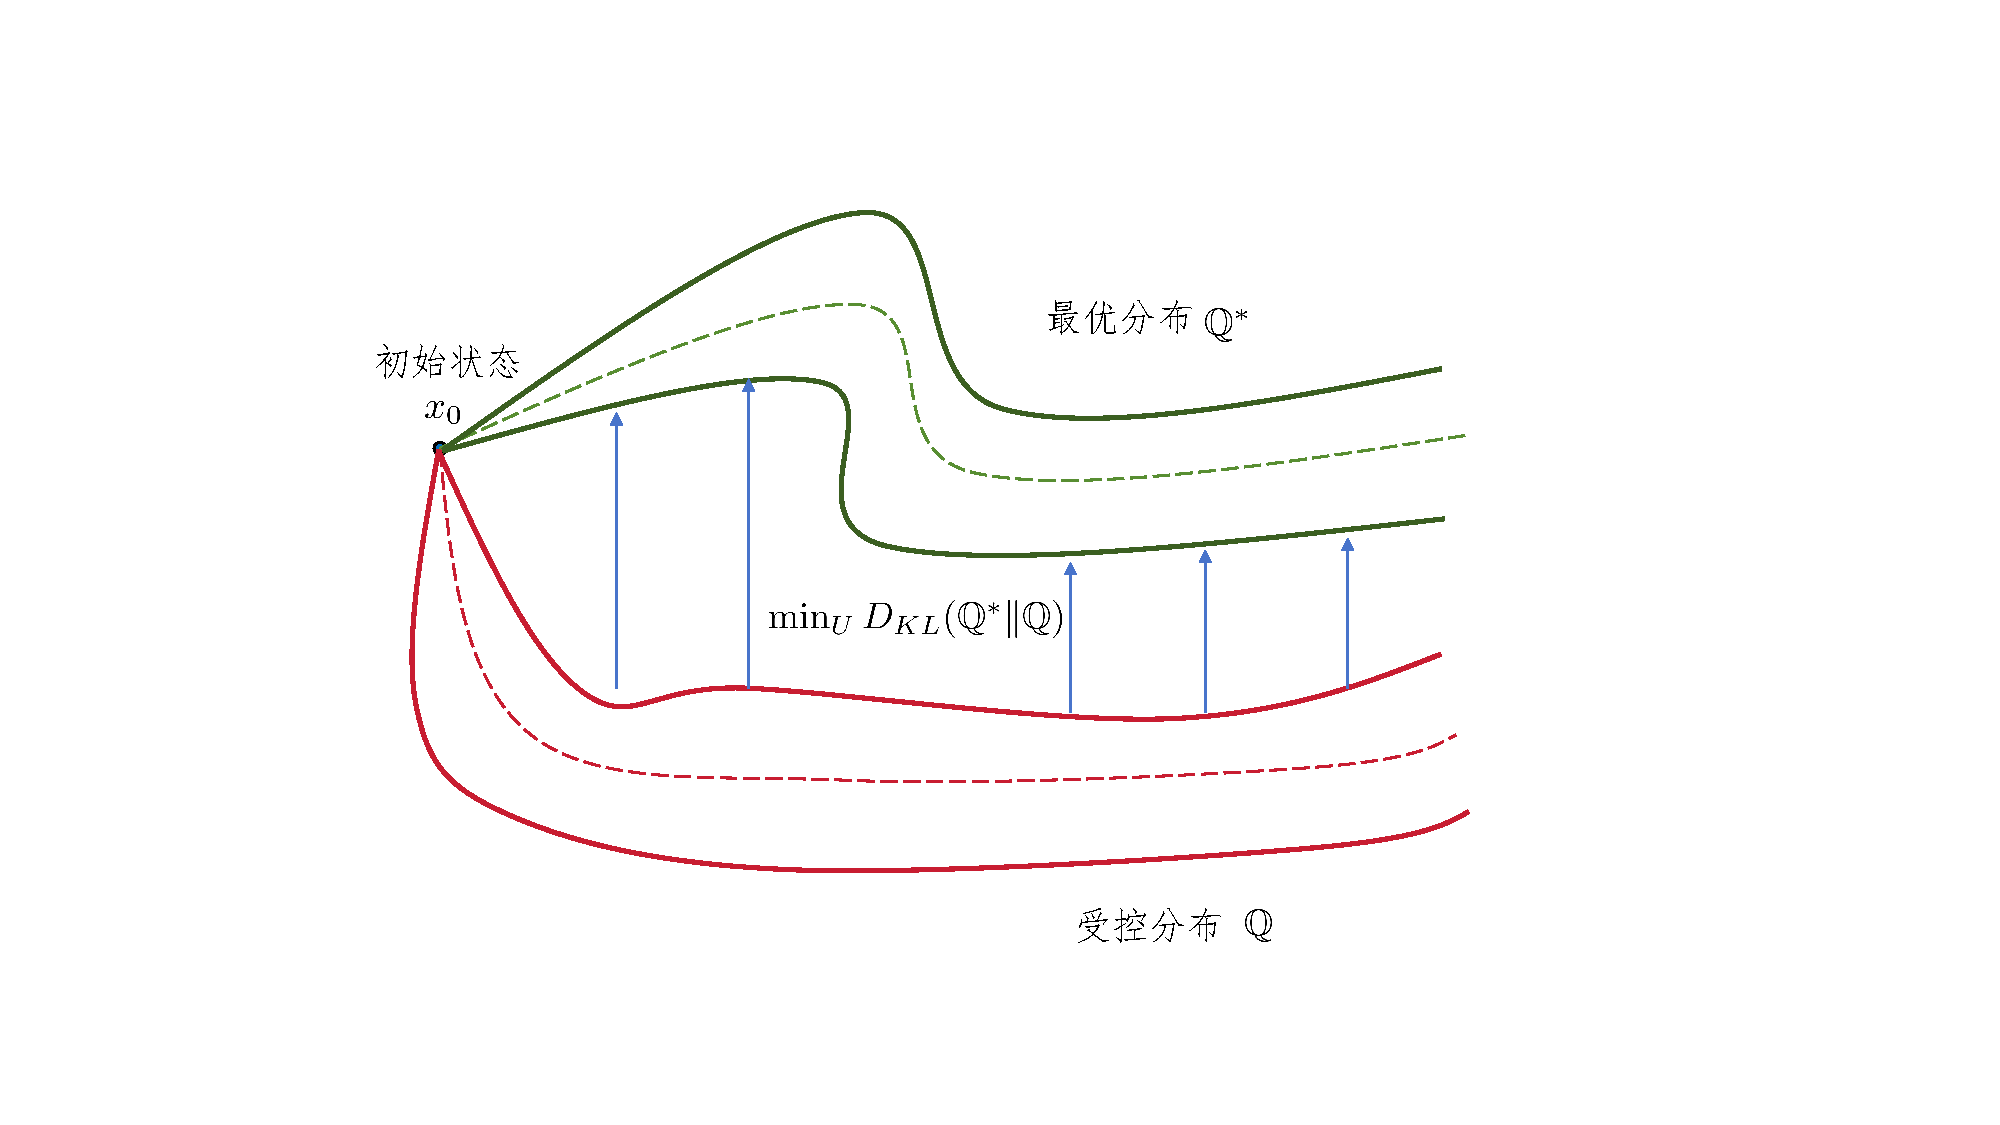
\includegraphics[width=0.6\textwidth]{figure/chapter4/distribution.pdf}
    \caption{最优分布与受控分布示意图}
    \label{fig:distribution}
\end{figure}
因此，最优控制问题转化为如下优化问题，如图\ref{fig:distribution}所示：
\begin{equation}
\begin{aligned}
    U^*=&\arg\min_U D_{KL}(\mathbb{Q}^* \Vert \mathbb{Q})
\end{aligned}
\end{equation}
因此可以将上述优化问题展开为：
\begin{equation}
\begin{aligned}
    U^*= &\arg\min_U\int q^*(V) \log \left(\frac{q^*(V)}{q(V)}\right) dV\\
    =&\arg\min_U\int q^*(V) \log \left(\frac{q^*(V)}{p(V)}\frac{p(V)}{q(V)}\right) dV\\
    =&\arg\min_U\int q^*(V) \log \left(\frac{q^*(V)}{p(V)}\right) - q^*(V)\log \left(\frac{q(V)}{p(V)}\right) dV
\end{aligned}
\end{equation}
可以发现，第一项与控制序列$U$无关，舍弃第一项后带入公式（\ref{equ:distribution}），优化目标可以简化为：
\begin{equation}
\begin{aligned}
    U^*=&\arg\max_U \int q^*(V) \sum_{t=0}^{T-1} \left[-\frac{1}{2}u_t^\top \Sigma^{-1} u_t + u_t^\top \Sigma^{-1} v_t\right] dV\\
    =&\arg\max_U \sum_{t=0}^{T-1} \left[-\frac{1}{2}u_t^\top \Sigma^{-1} u_t + u_t^\top \int q^*(V) \Sigma^{-1} v_t dV\right]\\
\end{aligned}
\end{equation}
上述优化问题是一个标准的二次规划，有解析解：
\begin{equation}
\begin{aligned}
    u_t^* = \int q^*(V) v_t dV
\end{aligned}
\end{equation}

然而，我们无法从最优分布$\mathbb{Q}^*$中直接采样，因此可以将上述积分重写为：
\begin{equation}
\begin{aligned}
    \int q^*(V) v_t dV=&\int q(V) \frac{q^*(V)}{p(V)} \frac{p(V)}{q(V)}v_t dV\\
\end{aligned}
\end{equation}
即最优控制序列可以通过从任意分布$\mathbb{Q}$中采样来近似计算：
\begin{equation}
\begin{aligned}
    &u_t^* = \mathbb{E}_{\mathbb{Q}}\left[w(V)v_t\right] \\
    &w(V) = \frac{q^*(V)}{p(V)} \frac{p(V)}{q(V)}
\end{aligned}
\end{equation}
带入公式（\ref{equ:optimal-distribution}）与公式（\ref{equ:distribution}），重要性采样权重$w(V)$可以表示为：
\begin{equation}
\begin{aligned}
    w(V)=\frac{1}{Z} \exp \left(-\frac{1}{\lambda}S(V) + \sum_{t=0}^{T-1} -v_t^\top \Sigma^{-1} u_t + \frac{1}{2} u_t^\top \Sigma^{-1} u_t \right)
\end{aligned}
\end{equation}
其中$Z$可以使用蒙特卡洛方法来近似计算：

\begin{equation}
\begin{aligned}
    Z = \sum_{n=1}^{K} \exp \left(-\frac{1}{\lambda}S(V) + \sum_{t=0}^{T-1} -v_t^\top \Sigma^{-1} u_t + \frac{1}{2} u_t^\top \Sigma^{-1} u_t \right)
\end{aligned}
\end{equation}
其中，$K$为使用$V$采样得到的轨迹样本数量。综上，名义控制序列的迭代更新法则为：
\begin{equation}
\begin{aligned}
    U_{i} = \sum_{k=1}^{K} w(V_k)V_k
\end{aligned}
\end{equation}
其中$i$表示第$i$次迭代，$V_k$表示第$k$条采样得到的实际控制序列。MPPI算法的具体流程如算法\ref{algo:mppi}所示。
\begin{algorithm}[ht]
    \begin{spacing}{1.25}
	\caption{MPPI控制算法}
    \renewcommand{\arraystretch}{1.25}
	\label{algo:mppi}
	\begin{algorithmic}[1]
        \REQUIRE 预测模型$\hat{p}$，采样数$K$，迭代数$N_{iter}$，预测时域$T$，控制器参数$q(), \phi(), \Sigma, \lambda$
        \ENSURE 最优控制序列$U^*$
        \STATE 初始化名义控制序列$U_0$，获得初始状态$x_0$
		\FOR{$i=1, 2, \cdots, N_{iter}$}{
            \FOR{$k=1, 2, \cdots, K$}{
                \STATE 根据名义控制序列$U_{i-1}$采样实际控制序列$V_k=\left\{v_0^k, v_1^k, \cdots, v_{T-1}^k\right\}$
                \STATE $x\leftarrow x_0$，$S(V_k) \leftarrow 0$
                \FOR{$t =1, 2, \cdots, T$}{
                    \STATE $x_t \leftarrow \hat{p}(x_{t-1}, v_{t-1}^k)$
                    \STATE $S(V_k) \leftarrow S(V_k) +q(x_t) + \frac{1}{2} (v_{t-1}^k)^\top R v_{t-1}^k -\frac{\lambda}{2} (2v_{t-1}^{k}-u_{t-1})^\top \Sigma^{-1} u_{t-1}$
                }\ENDFOR
                \STATE $S(V_k) \leftarrow S(V_k) + \phi(x_T)$
            }\ENDFOR
            \STATE $\beta \leftarrow \min_k [S(V_k)]$
            \STATE $Z \leftarrow \sum_{k=1}^{K} \exp \left(-\frac{1}{\lambda}(S(V_k) - \beta)\right)$
            \FOR{$k=1, 2, \cdots, K$}{
                \STATE $w(V_k) \leftarrow \frac{1}{Z} \exp \left(-\frac{1}{\lambda}(S(V_k) - \beta)\right)$
            }\ENDFOR
            \STATE 更新名义控制序列$U_i \leftarrow \sum_{k=1}^{K} w(V_k)V_k$
        }\ENDFOR
        \RETURN 最优控制序列$U^* = U_{N_{iter}}$
	\end{algorithmic}
    \end{spacing}
\end{algorithm}

\subsection{导航控制的奖励函数设计}
为了将MPPI算法和VPM结合起来，本文需要设计一个合适的奖励函数来评估不同控制序列的长期奖励。奖励函数的设计需要考虑到导航任务的目标和约束条件。一般来说，导航任务的目标是使机器人能够快速、安全地到达目标位置，同时避免碰撞和其他危险情况。因此，本节将奖励函数设计为以下几个部分：
\begin{itemize}
    \item \textbf{目标位置奖励：}当机器人接近目标位置时，给予正奖励；当机器人远离目标位置时，给予负奖励。鼓励机器人快速朝着目标位置移动。
    \item \textbf{速度奖励：}在目标值周围适当给速度惩罚，保证机器人可以以较高的速度移动，同时在接近目标位置时减速，以实现更精确的停靠。
    \item \textbf{碰撞惩罚：}为了避免碰撞和其他危险情况，本文设计了一个碰撞惩罚，当机器人发生碰撞或者接近障碍物时，给予负奖励。
    \item \textbf{平滑控制奖励：}为了使控制序列更加平滑，本文设计了一个平滑控制奖励，当控制输入变化较大时，给予负奖励；当控制输入变化较小时，给予正奖励。
\end{itemize}
综上，奖励函数可以写为以下形式：
{
\allowdisplaybreaks
\begin{subequations}
\begin{align}
    &r(x_t, u_t) = r_{\text{goal}} +  r_{\text{speed}} +  r_{\text{collision}} + r_{\text{smooth}} \\
    &r_{\text{goal}} = -w_1 \Vert \hat{p}_t - g \Vert^2 \\
    &r_{\text{speed}} = w_2\Vert \hat{v}_t \Vert^2 \cdot \exp(-\alpha \Vert \hat{p}_t - g \Vert^2) \\ \label{subequ:speed-penalty}
    &r_{\text{collision}} = -w_3\mathbb{I}(\hat{c}_t) \\
    &r_{\text{smooth}} = -(u_t - u_{t-1})^\top R_{\Delta u} (u_t - u_{t-1}) \label{subequ:control-smooth}
\end{align}
\end{subequations}
}
其中，$g$表示目标位置，$\hat{p}_t$表示机器人在时间步$t$的预测位置，$\hat{v}_t$表示机器人在时间步$t$的预测速度，$\hat{c}_t$表示机器人在时间步$t$的碰撞状态，$u_t$表示机器人在时间步$t$的控制输入，$\mathbb{I}(\cdot)$是指示函数，$w_1$、$w_2$、$w_3$和$w_4$是不同奖励项的权重系数，可以根据具体的任务需求进行调整。为了将奖励函数转换为代价函数，定义代价函数为奖励函数的负值，即：
\begin{equation}
\begin{aligned}
    S(\tau) &= -\sum_{t=0}^{T-1} r(x_t, u_t) + \phi(x_T) \\
    \phi(x_T) &= w_{T, p} \Vert \hat{p}_T - g \Vert^2 + w_{T, v} \Vert \hat{v}_T \Vert^2
\end{aligned}
\end{equation}
其中，$\phi(x_T)$是终端代价，用于鼓励机器人在时间步$T$时接近目标位置，$w_{T, p}$，$w_{T, v}$是终端代价的权重系数。这样的奖励函数可以引导MPPI算法基于VPM选择能够实现高速、安全导航的控制序列。

\section{仿真与实车实验}
本节首先进行了基于仿真环境的导航控制实验，验证了基于视觉预测模型的MPPI方法在高速导航任务中的性能。随后，本节进行了消融实验，分析了不同设计对导航性能的影响。最后，本节在实车上进行了验证实验，展示了该方法在现实环境中的有效性。
\subsection{导航效果对比实验}
\begin{figure}[ht]
    \centering
    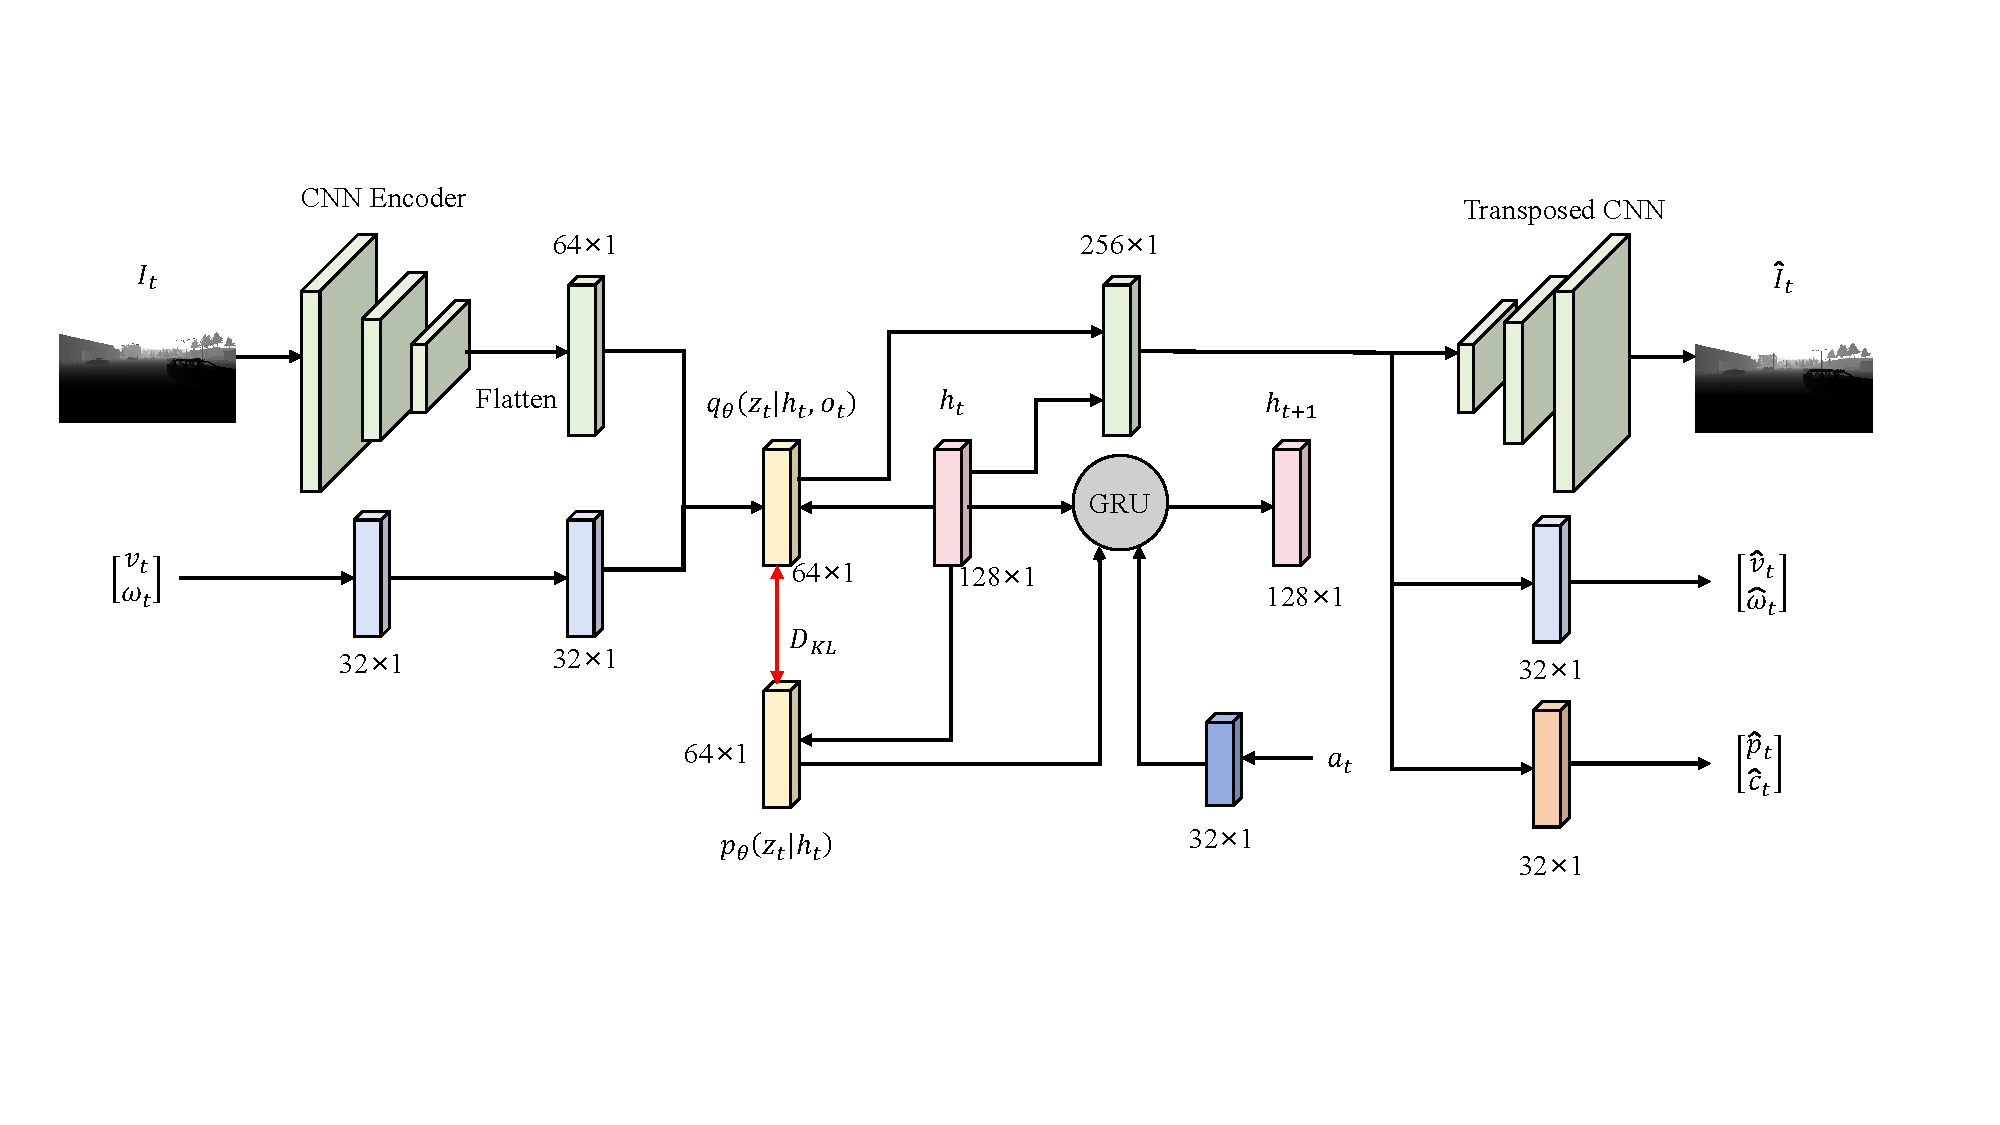
\includegraphics[width=1.0\textwidth]{figure/chapter4/model-archi.pdf}
    \caption{视觉预测模型网络细节}
    \label{fig:model-architecture}
\end{figure}
仿真实验只使用了仿真环境中的数据来训练VPM，并使用MPPI方法进行导航控制。深度图像像素值被归一化到$[0, 1]$范围内，图像的大小为$64\times 96$。图像经三层卷积层和两层全连接层处理后，与运动状态$\beta_t$拼接后可以得到后验分布$q_{\theta}(z_t\vert o_t, h_t)$。先验分布$p_{\theta}(z_t\vert h_t)$由两层全连接层处理后得到。状态转移模型$f_{\theta}$由一个GRU单元构成，输入为随机状态$z_t$和动作$u_t$，输出确定性状态$h_{t+1}$。图像重建模型包括两层全连接层和三层反卷积层，运动状态重建模型由两层全连接层构成。状态预测模型由两层全连接层构成。整个模型的结构设计如图\ref{fig:model-architecture}所示。仿真中的训练采用了Adam优化器，学习率为$1e-3$，批次大小为$256$。
\begin{table}[h]
    \caption{\label{tab:mppi-params}MPPI控制器参数}
    \renewcommand\arraystretch{1.2}
    \begin{tabularx}{\linewidth}{X<{\centering} X<{\centering} || X<{\centering} X<{\centering}}
    \toprule[2pt]
        参数 & 大小 & 参数 & 大小 \\ \midrule[1pt]
        $K$ & $600$ & $N_{iter}$ & $4$ \\
        $\lambda$ & $10.0$ & $\Sigma$ & $diag(2.0, 0.2)$ \\
        $w_1$ & $1.0$ & $w_2$ & $0.5$ \\
        $w_3$ & $1e^{10}$ & $\alpha$ & $2.0$ \\
        $R_{\Delta u}$ & $diag(1.0, 0.5)$ & $w_{T, p}$ & $10.0$ \\
        $w_{T, v}$ & $1.0$ & $T$ & $15$ \\
        采样时间 & $0.1 s$ & & \\
    \bottomrule[2pt]
    \end{tabularx}
\end{table}

MPPI控制器的参数设置如表\ref{tab:mppi-params}所示。在MPPI的实际操作中，仍有一些细节需要注意。首先，重要性采样的权重可能会出现数值不稳定的情况，特别是当代价函数的值较大时。为了缓解这个问题，本节在计算权重时引入了一个基于最小代价的偏移量$\beta$，即将代价函数的值减去$\beta$，从而避免了指数函数中的大数值问题，如算法\ref{algo:mppi}中所示。其次，温度参数$\lambda$的选择对于控制性能有重要影响。较小的$\lambda$会使得控制策略更加集中于低代价的轨迹，而较大的$\lambda$则会使得控制策略更加分散。本节通过实验调整$\lambda$的值，以找到一个能够平衡探索和利用的最佳设置，将于后续的消融实验中进行分析。另外，由于采样可能带来抖动的控制输入，本节在实际执行控制命令时，采用了Savitsky-Galoy滤波器\cite{savitzky1964smoothing}来平滑控制输入，从而提高控制的稳定性和舒适性。最后，MPPI算法的计算复杂度较高，特别是在采样数量较大时。为了满足实时控制的要求，本节在实验中采用了GPU并行计算的方式来加速采样、预测和计算代价函数的过程，确保能够在每个控制周期内完成MPPI算法的计算。VPM的训练和MPPI采样均在一台CPU为Intel Core i7-12700K，GPU为NVIDIA RTX 3090的计算机上进行。

本节选取了三个评价指标来评估基于VPM的MPPI方法在仿真环境中的导航性能：（1）平均到达时间（Average Time，简称AT）：机器人从起始位置到达目标位置所需的平均时间；（2）平均路径长度（Path Length，简称PL）：机器人从起始位置到达目标位置所经过的平均路径长度；（3）成功率（Success Rate，简称SR）：机器人成功到达目标位置的比例。

首先本节在CARLA仿真环境中构建了一个高速导航任务，机器人需要从起始位置快速、安全地到达目标位置。然后将基于VPM的MPPI方法（简称VPM-MPPI）与以下几种基线方法进行了对比：（1）基于PPO强化学习的导航方法，图像由卷积神经网络处理（简称PPO-CNN）；（2）基于PPO强化学习的导航方法，加入一个GRU单元来处理部分可观测信息（简称PPO-CNN-GRU）。CARLA中一共有两个环境：（1）停车场避障，（2）城市街道导航，每种方法在相同的仿真环境中进行了100次独立的导航试验，并记录了上述三个评价指标。表\ref{table:carla-comparison}展示了不同方法在CARLA仿真环境中的导航性能比较结果。可以看出，VPM-MPPI在两个环境中都取得了最高的成功率，在平均到达时间和平均路径长度方面也表现出了明显的优势。此外，图\ref{fig:CARLA-comparison-traj}展示了不同方法在CARLA仿真环境中的导航轨迹比较，VPM-MPPI能够生成更平滑、更直接的导航轨迹，从而实现更高效的导航控制。
\begin{table}[ht]
\renewcommand{\arraystretch}{1.2}
\caption{CARLA仿真环境中不同方法的导航性能比较}
\centering
\setlength{\tabcolsep}{16pt}{
    \begin{tabular}{ccccc}%四个c代表该表一共四列，内容全部居中
    \toprule[2pt]
    \textbf{场景} & \textbf{方法} & SR[\%] & PL[$m$] & AT[$s$]\\
    \midrule[1pt]
    \multirow{3}{*}{停车场} & PPO-CNN & $0$ & - & - \\
    & PPO-CNN-GRU  & $62.5$ & $65.26\pm0.27$ & $19.74\pm0.09$ \\
    & VPM-MPPI  & $100$ & $58.32\pm0.34$ & $17.23\pm0.12$\\
    \midrule[1pt]
    \multirow{3}{*}{城市街道} & PPO-CNN & $20$ & $103.88\pm0.47$ & $22.64\pm0.11$\\
    & PPO-CNN-GRU  & $85$ & $103.34\pm0.69$ & $21.23\pm0.13$\\
    & VPM-MPPI  & $100$ & $102.39\pm0.75$ & $19.60\pm0.16$\\
    \bottomrule[2pt]
\end{tabular}}
\label{table:carla-comparison}
\end{table}
\begin{figure}[ht]
    \centering
    \subfloat[停车场]{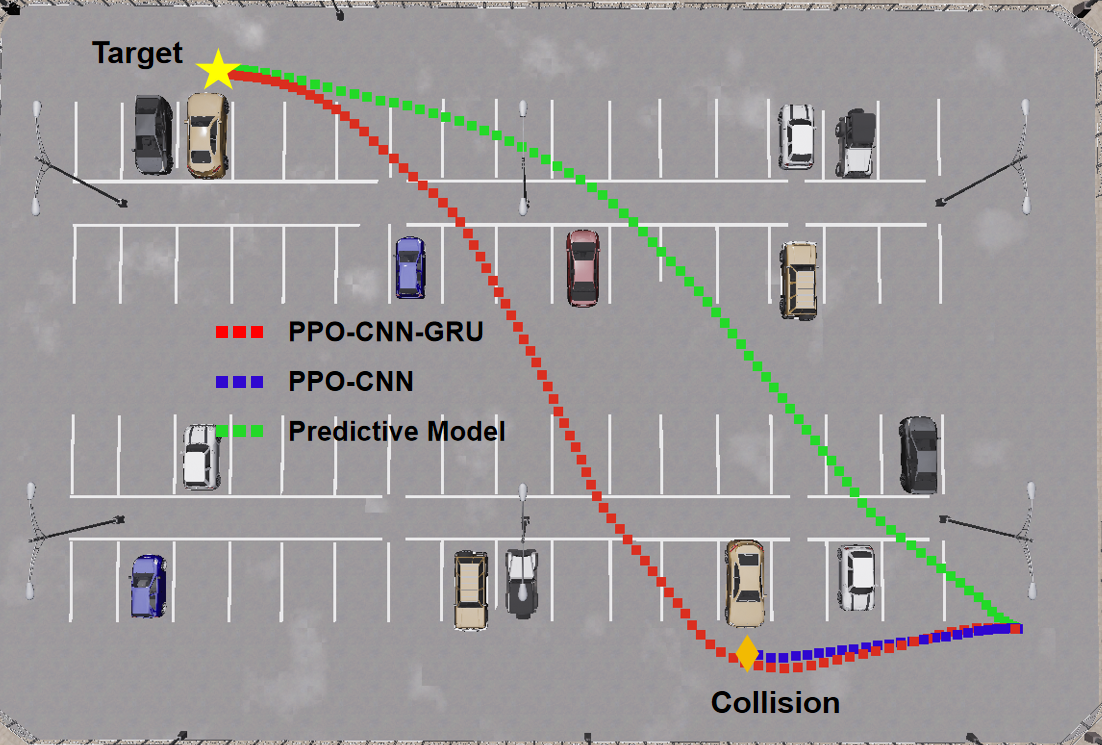
\includegraphics[width=0.39\linewidth]{figure/chapter4/traj11.png}}
    \subfloat[城市街道]{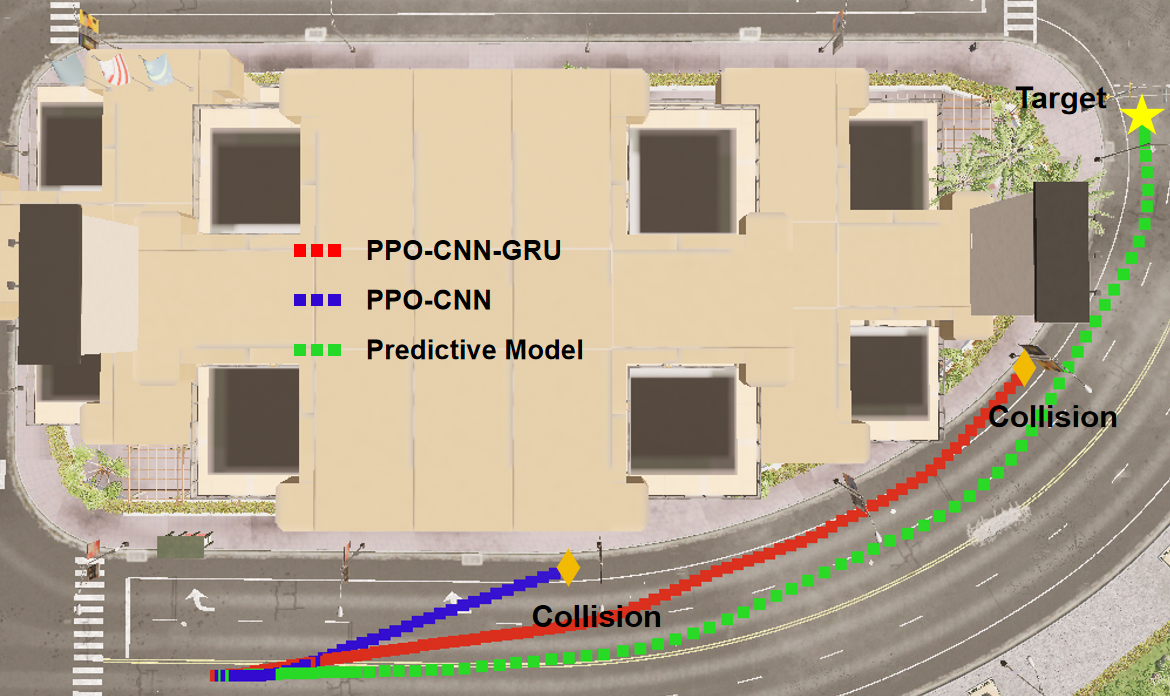
\includegraphics[width=0.442\linewidth]{figure/chapter4/traj22.png}}
    \caption{CARLA仿真环境中不同方法的导航轨迹比较}
    \label{fig:CARLA-comparison-traj}
\end{figure}

\begin{figure}[ht]
    \centering
    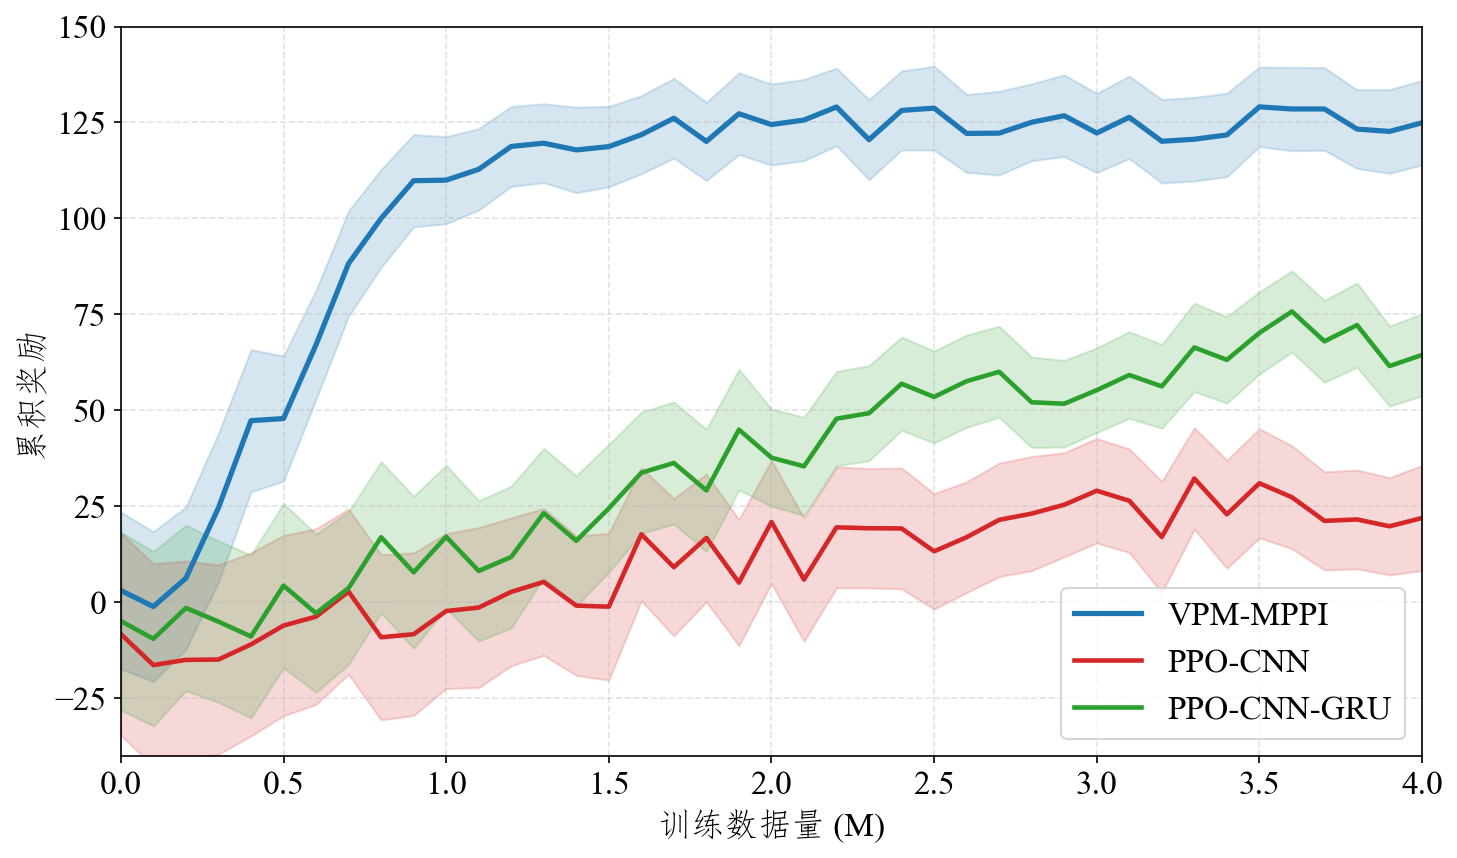
\includegraphics[width=0.6\textwidth]{figure/chapter4/reward_comparison.png}
    \caption{CARLA仿真环境中不同方法的累积奖励比较}
    \label{fig:reward-comparison}
\end{figure}
此外，本节还比较了不同方法在训练过程中的累积奖励表现，如图\ref{fig:reward-comparison}所示。可以看出，VPM-MPPI在1.5M训练步后，累积奖励已达到了一个较高水平，并且在后续的训练过程中保持了稳定的表现。而基于PPO的方法在训练初期表现较差，随着训练的进行，累积奖励逐渐提升，但仍然无法达到VPM-MPPI的水平。这进一步验证了本章方法在数据效率上的优势。

\begin{figure}[ht]
    \centering
    \subfloat[稀疏环境中的运行轨迹]{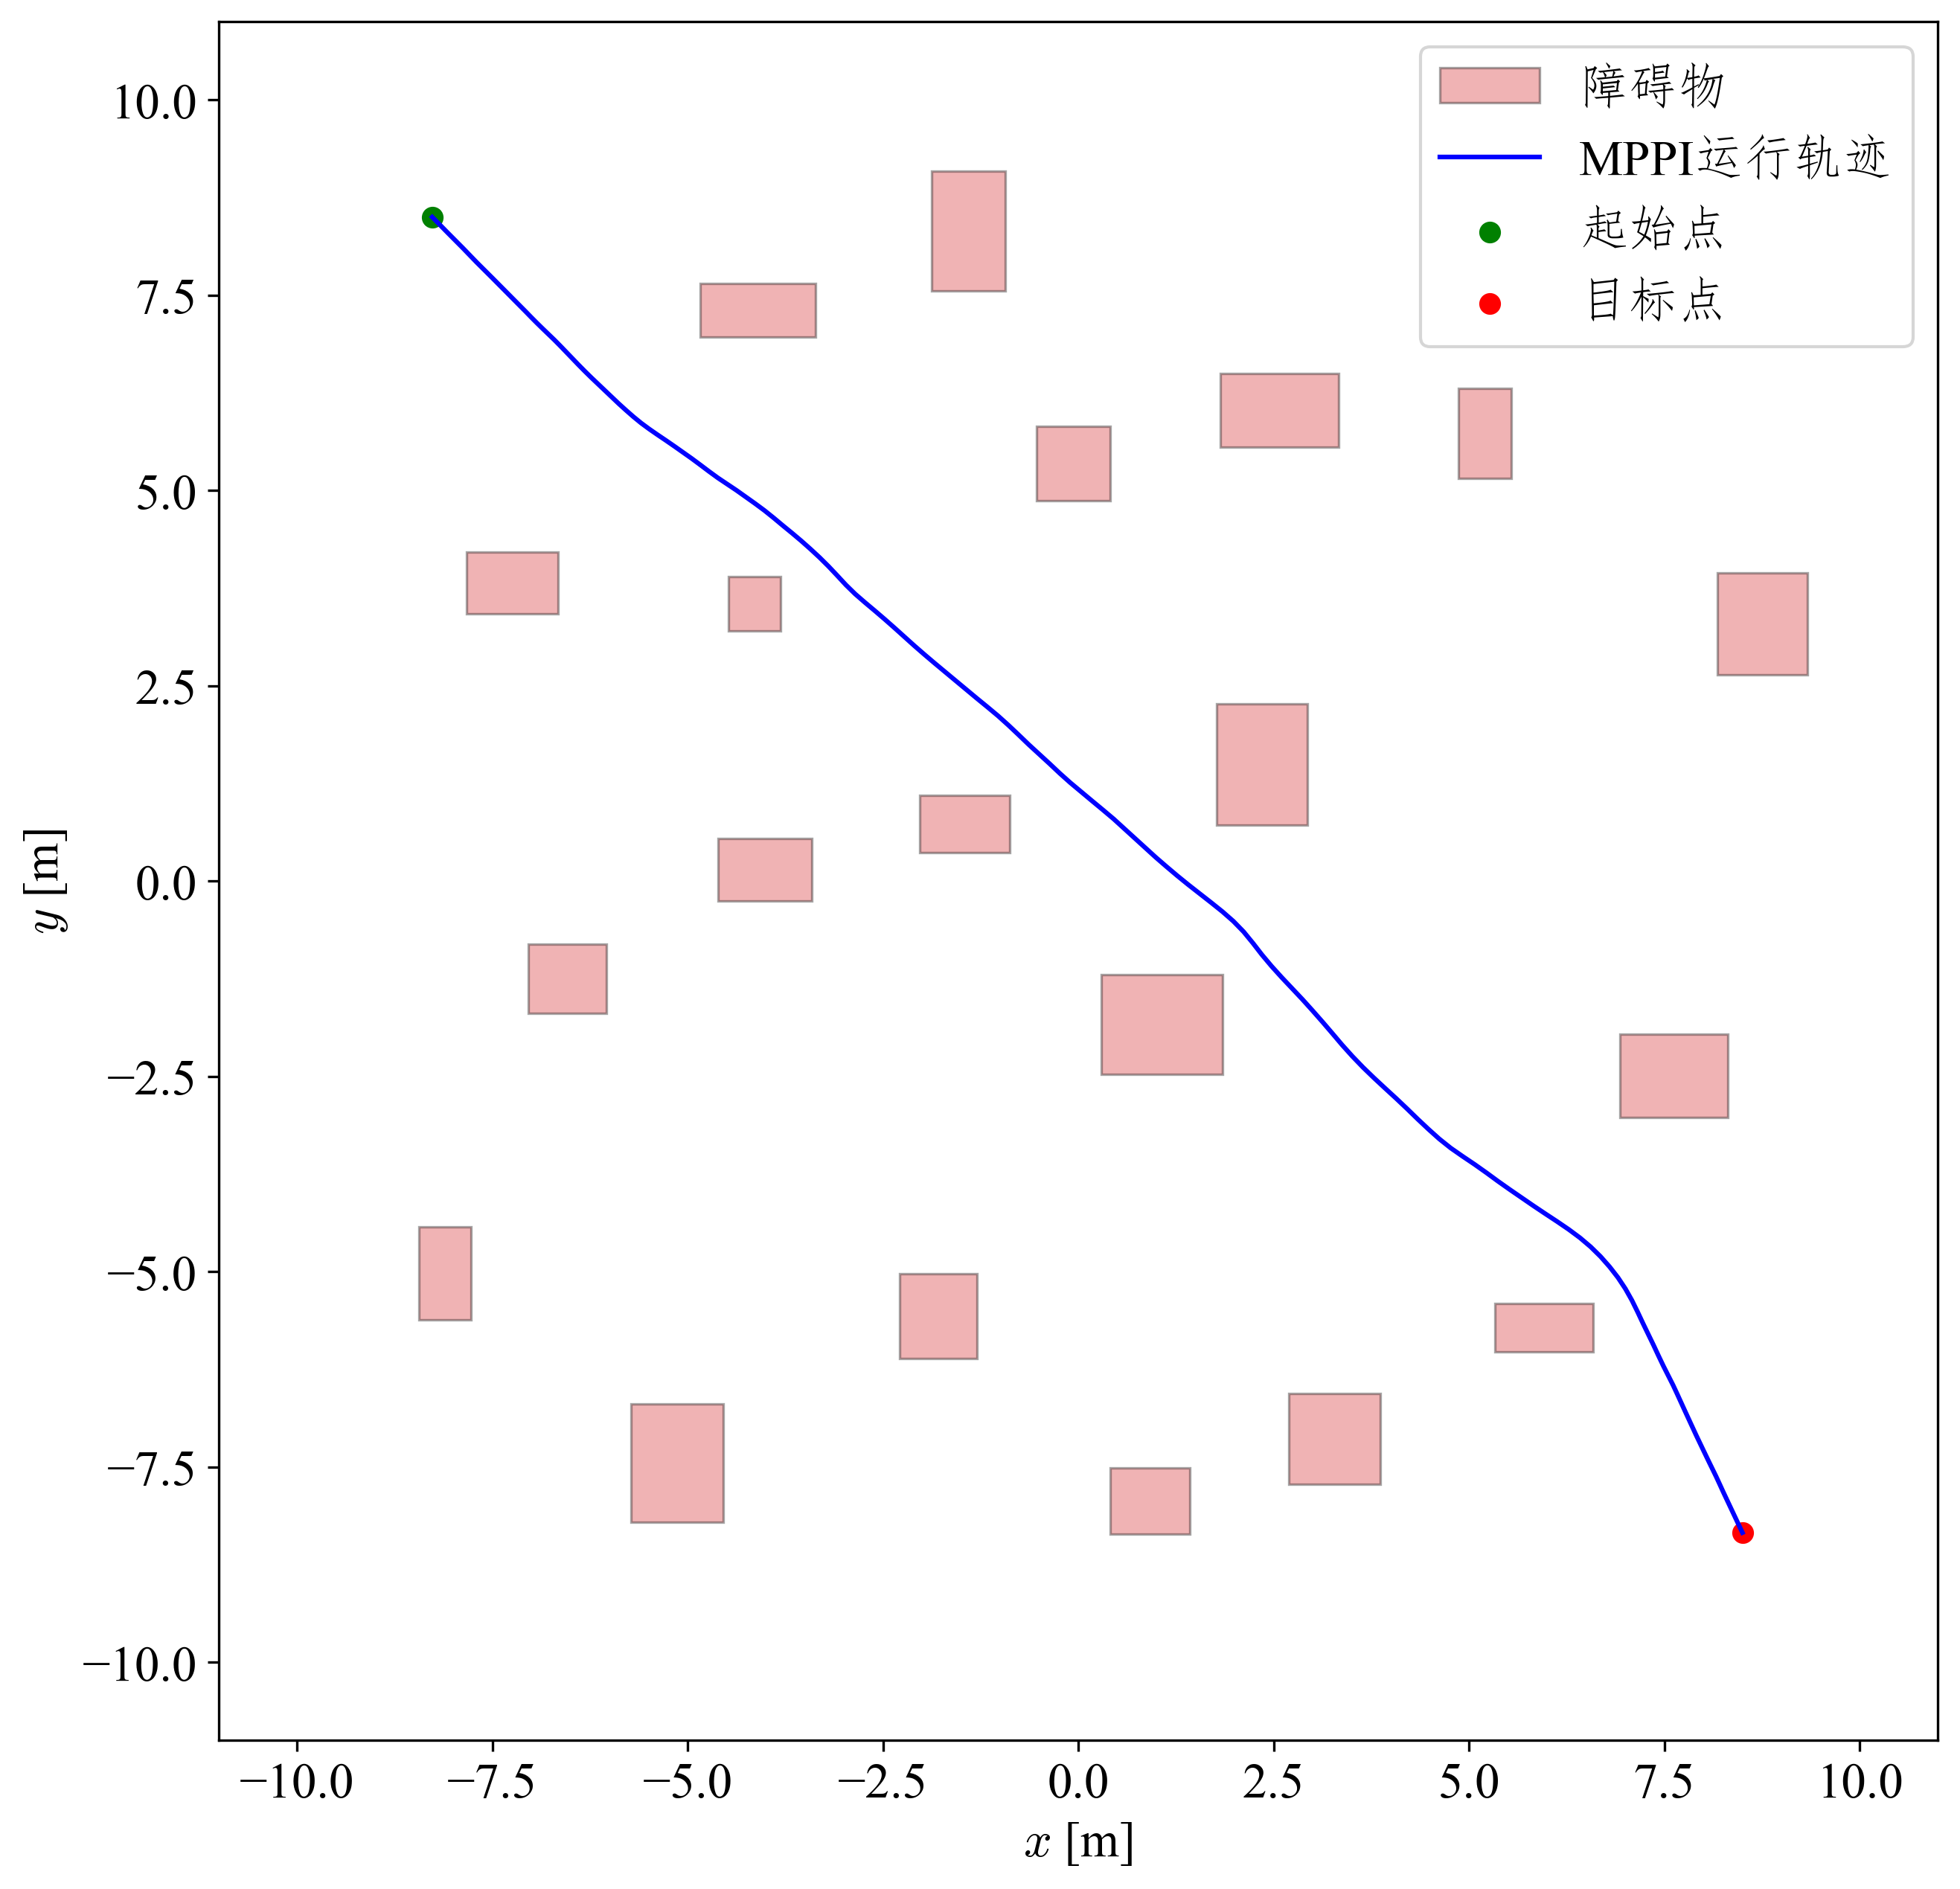
\includegraphics[width=0.33\linewidth]{figure/chapter4/mppi_trajectory_sparse.png}}
    \subfloat[中等环境中的运行轨迹]{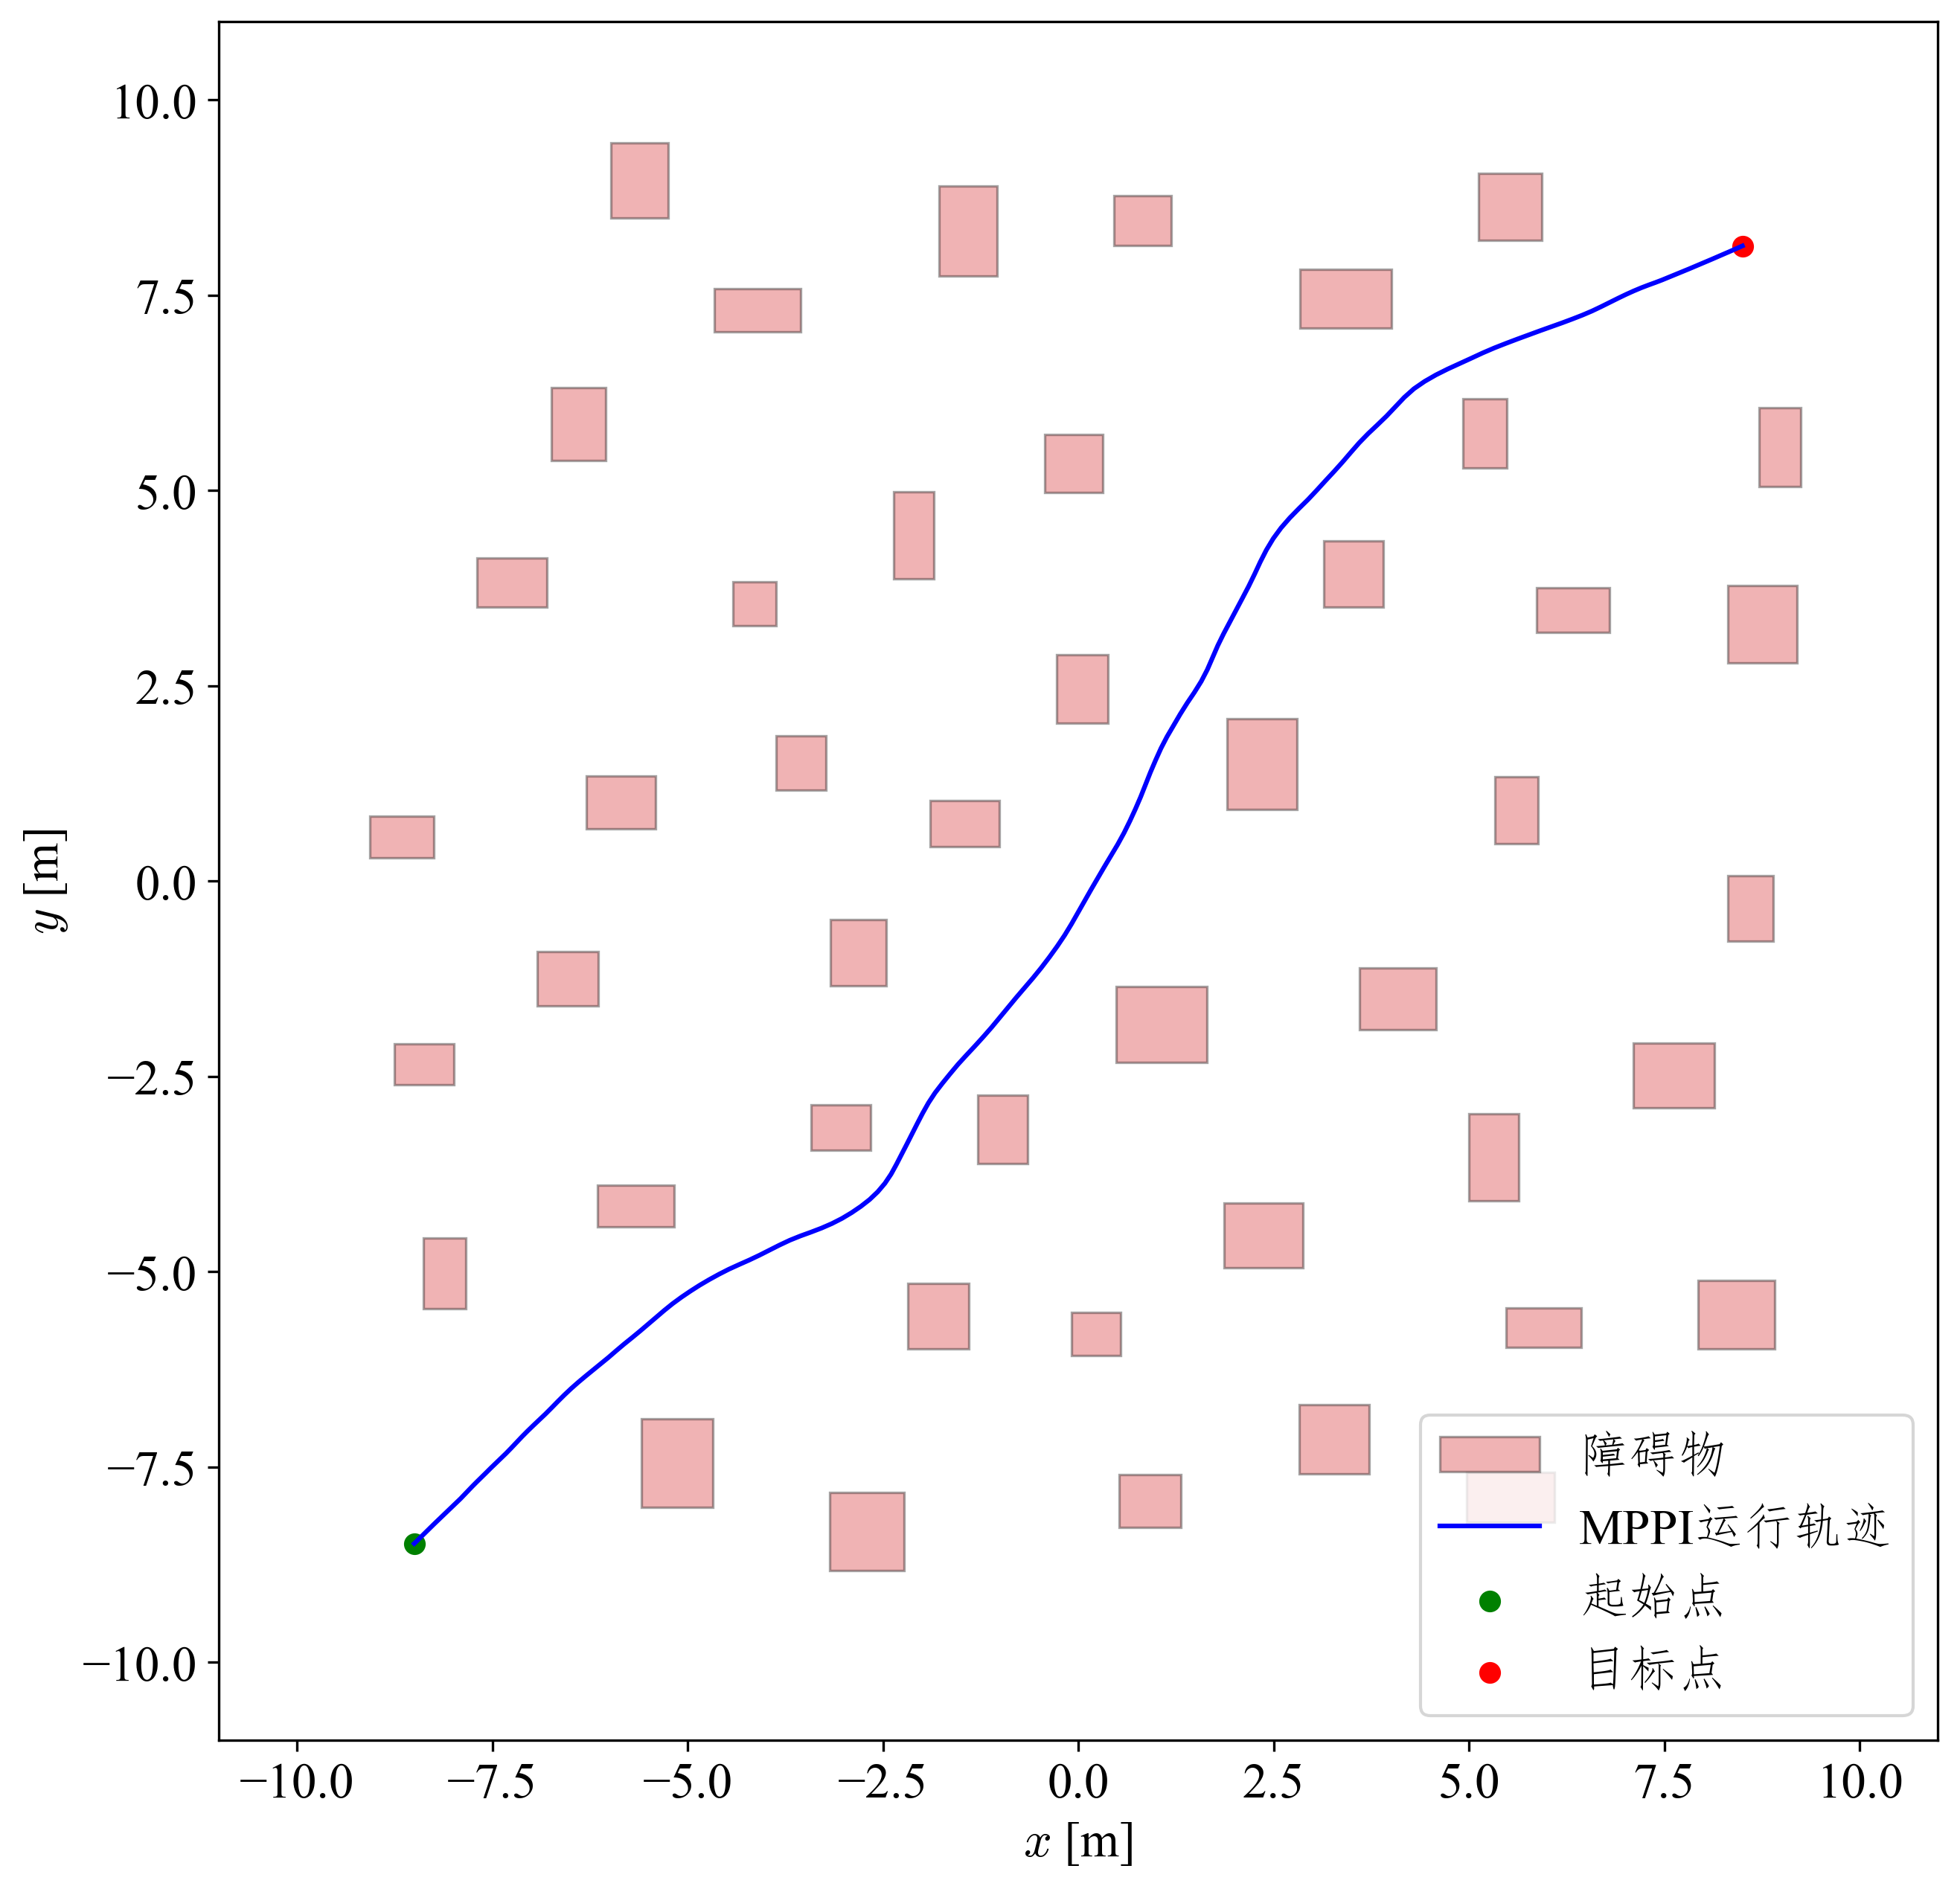
\includegraphics[width=0.33\linewidth]{figure/chapter4/mppi_trajectory_medium.png}}
    \subfloat[稠密环境中的运行轨迹]{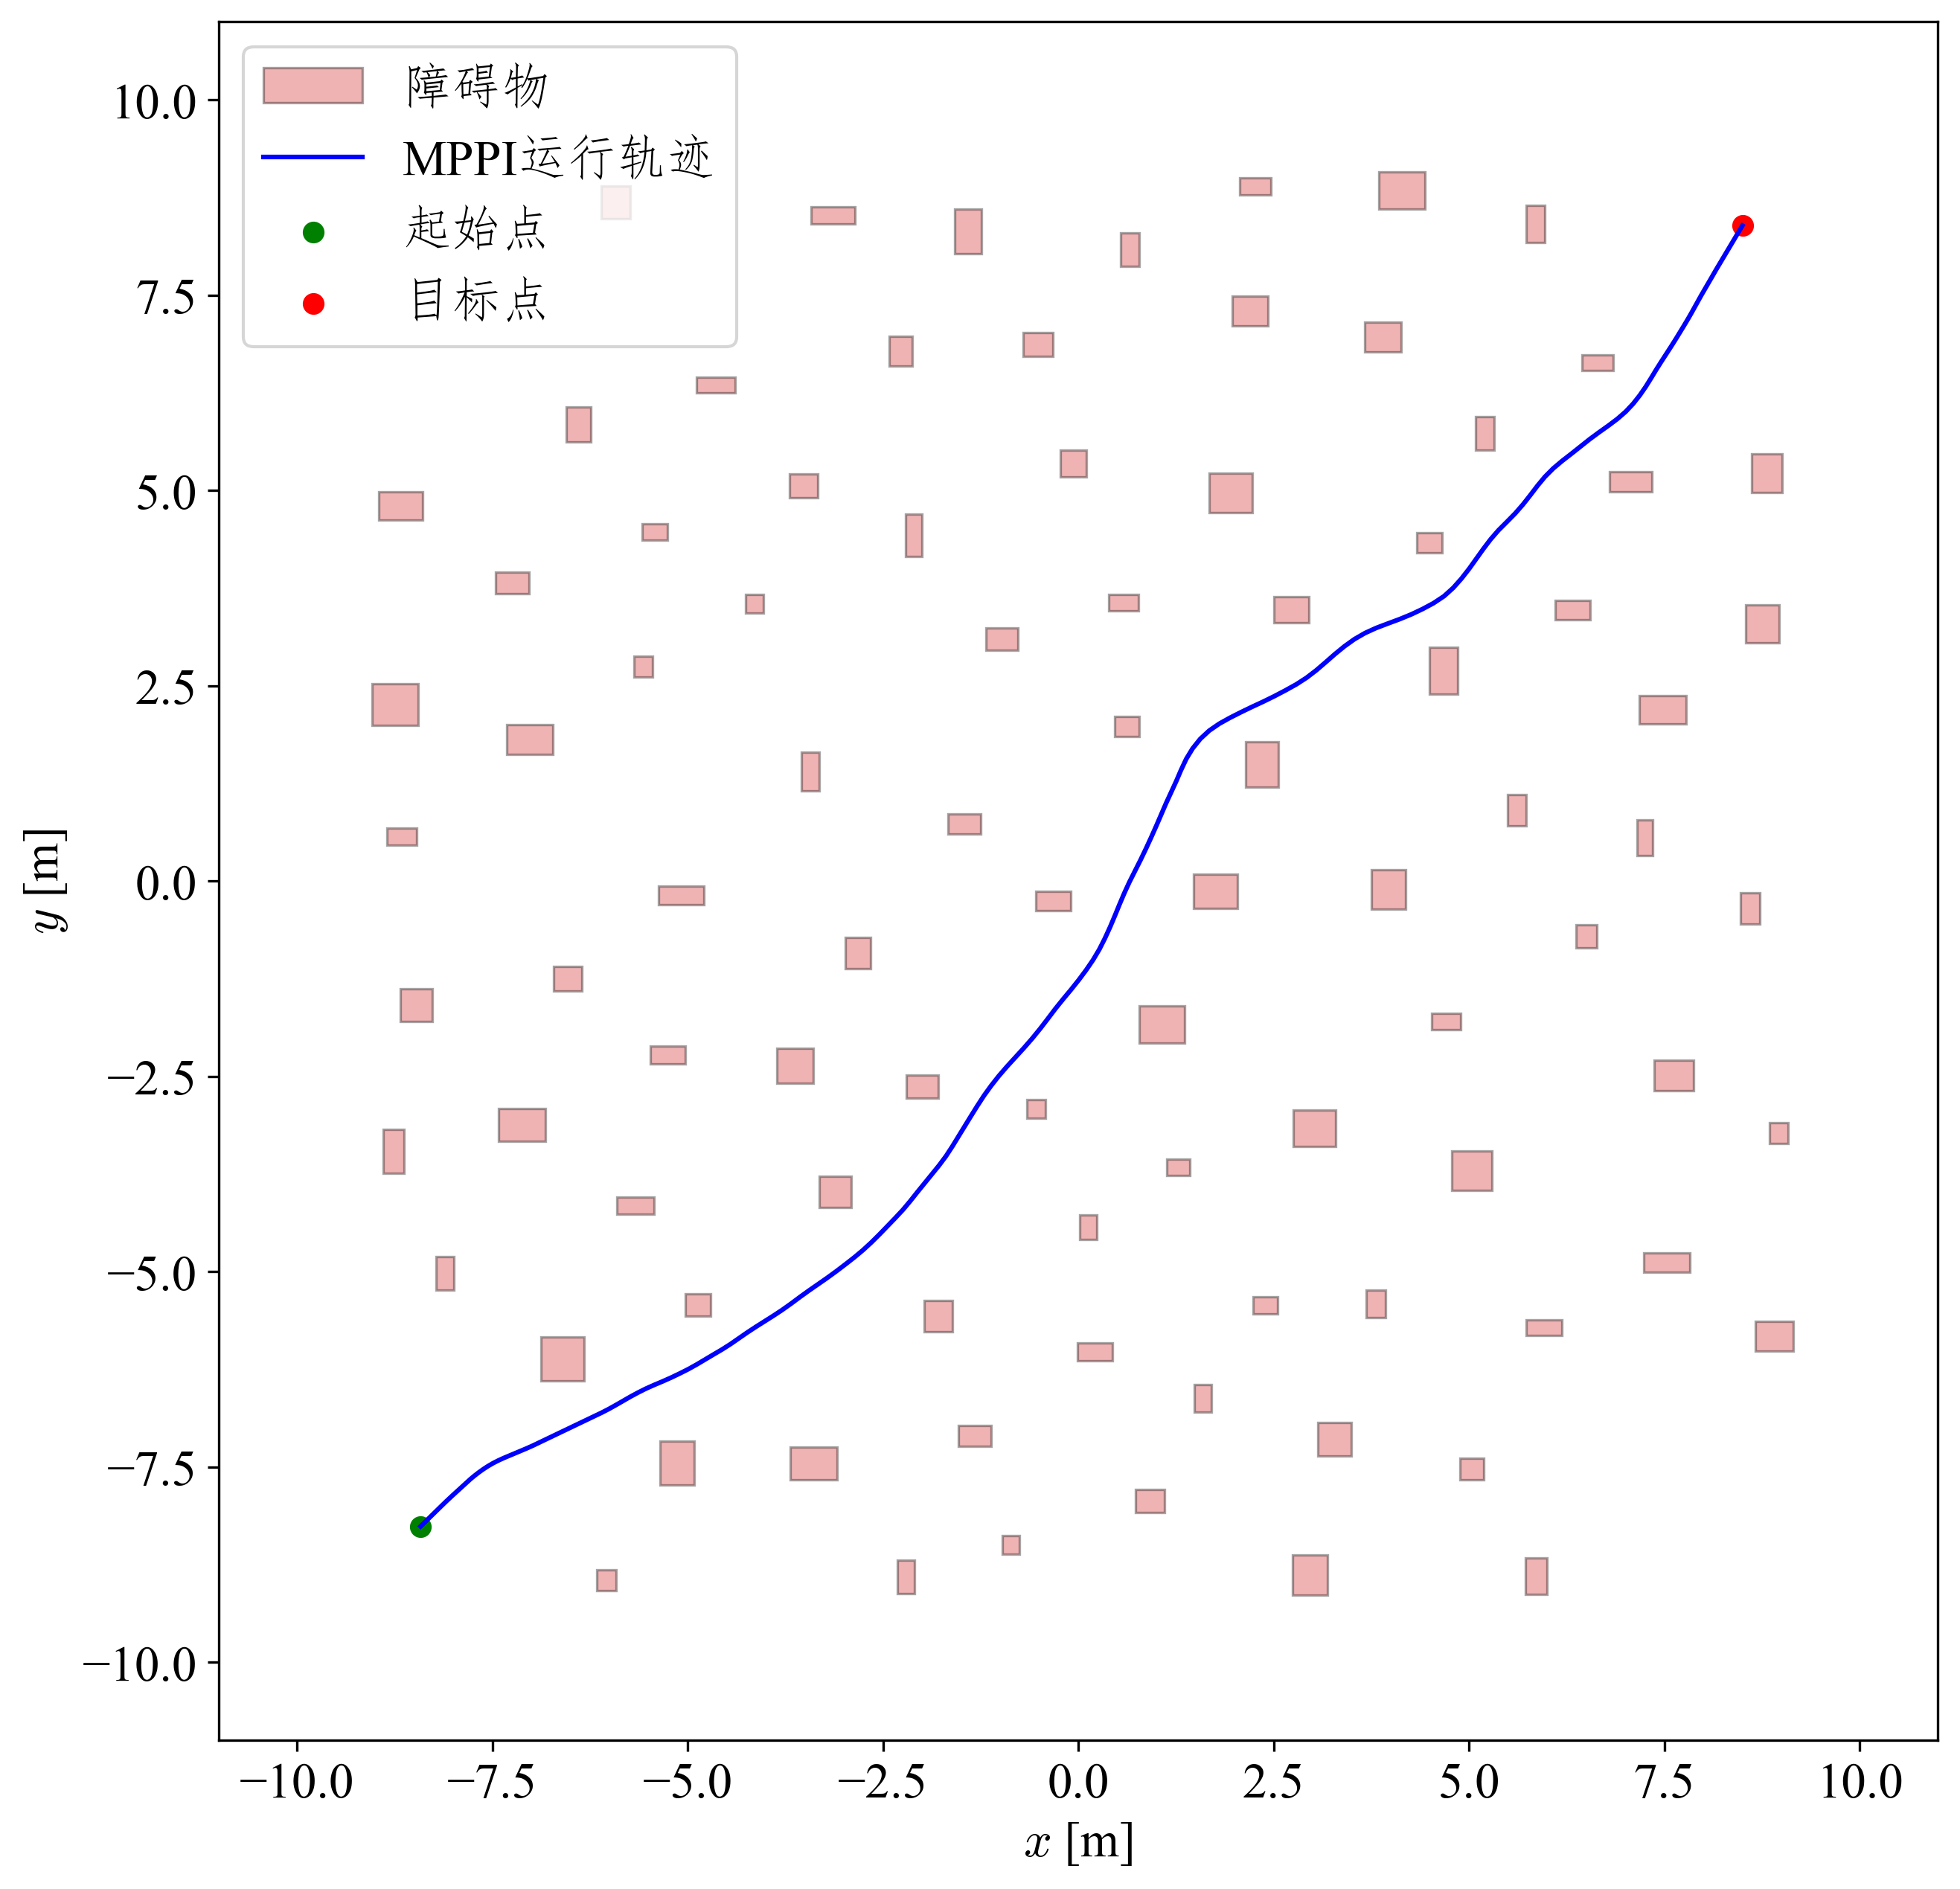
\includegraphics[width=0.33\linewidth]{figure/chapter4/mppi_trajectory_dense.png}}

    \subfloat[稀疏环境中的控制量]{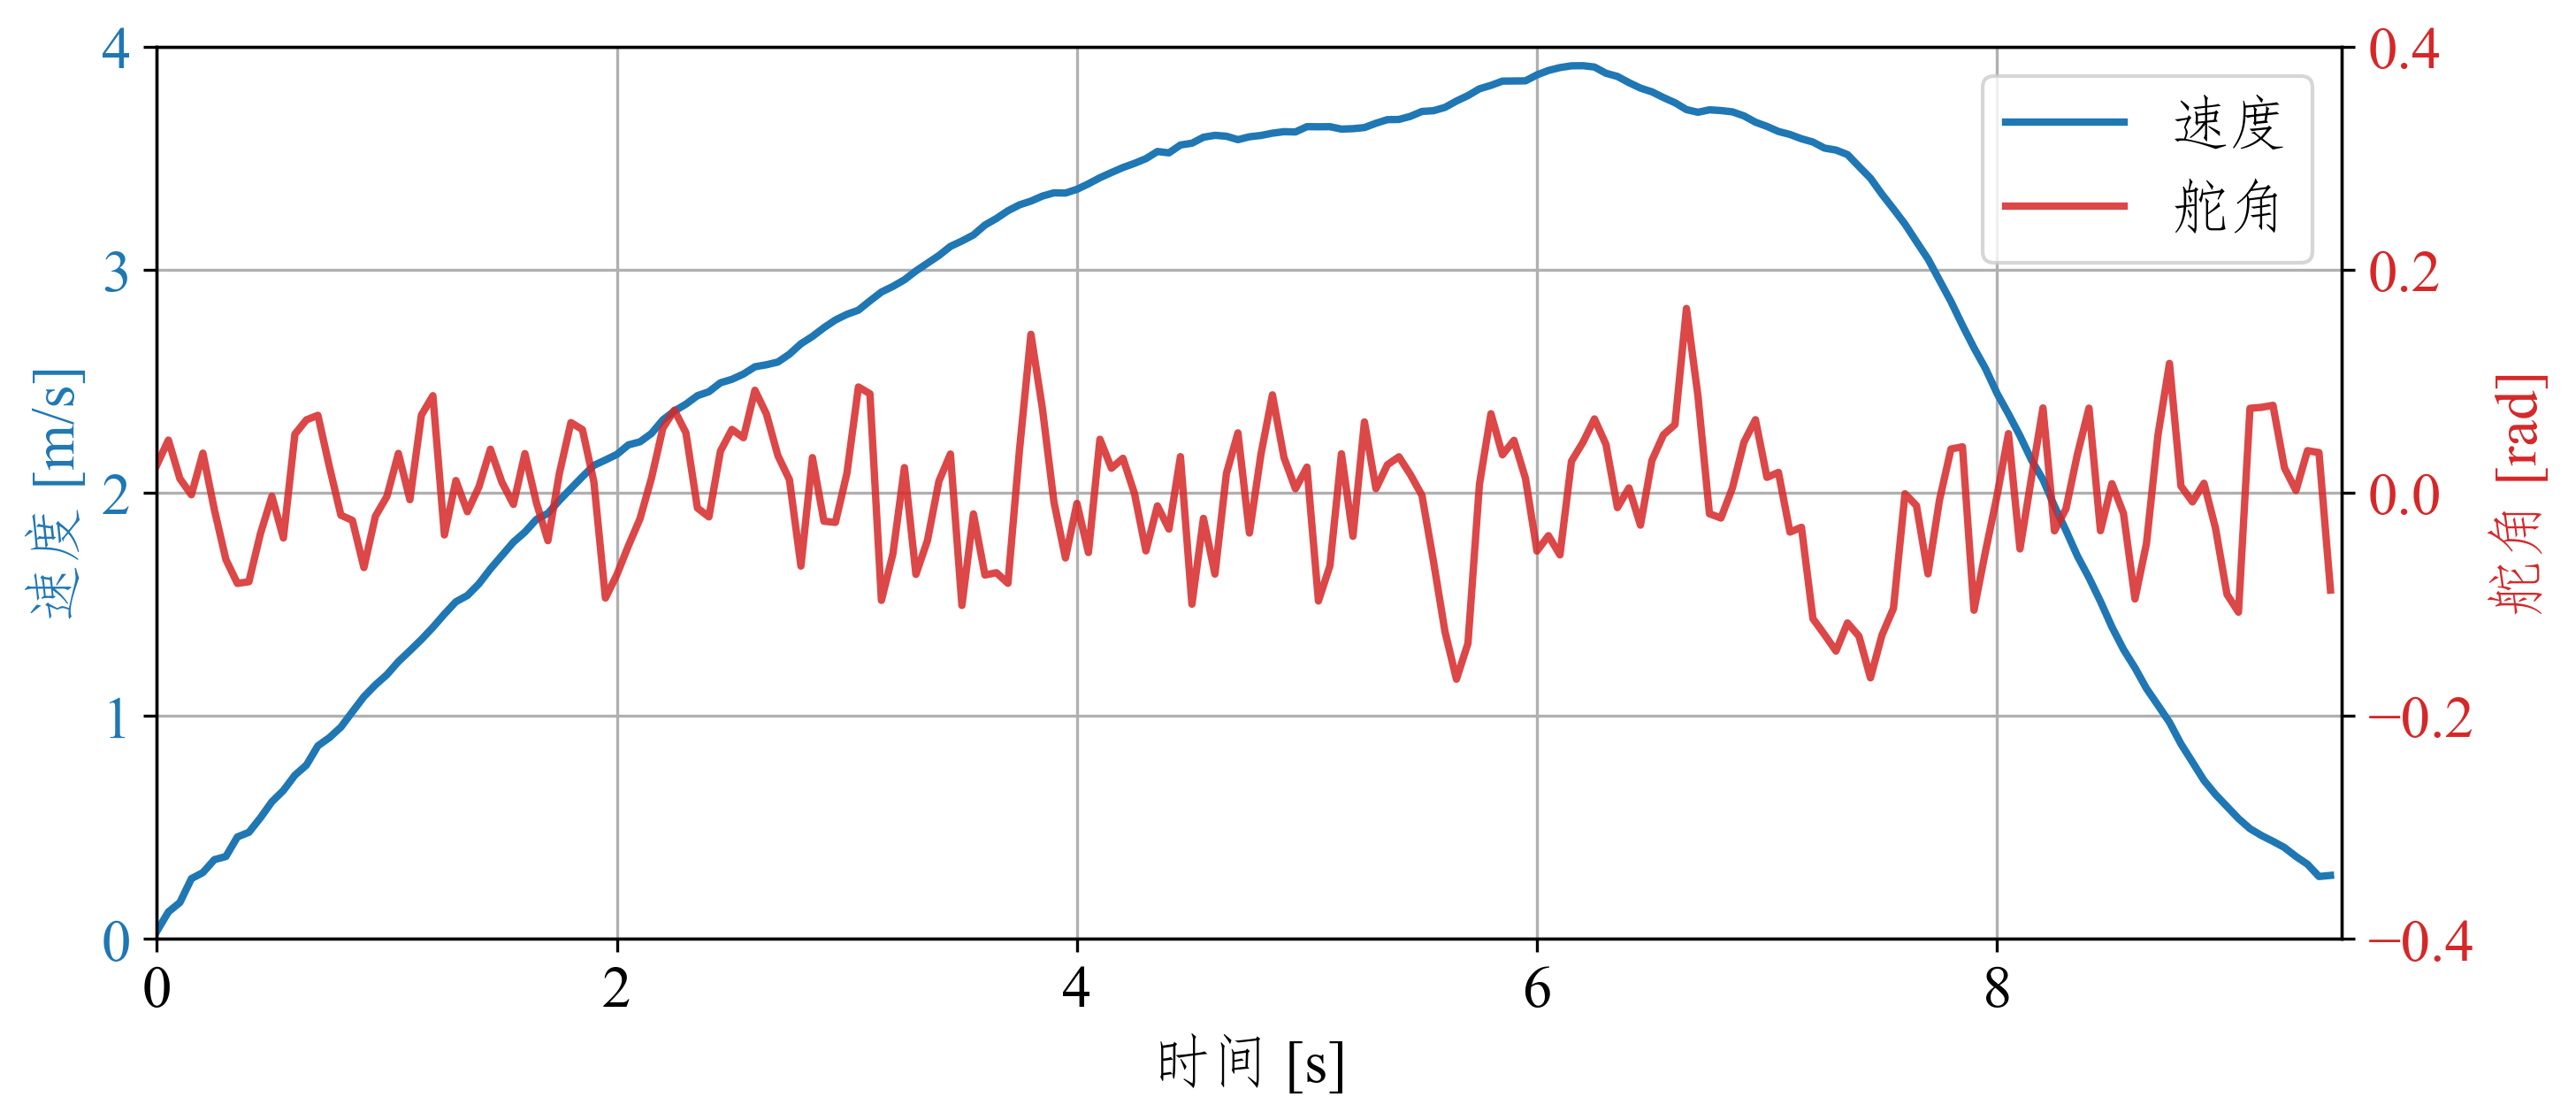
\includegraphics[width=0.33\linewidth]{figure/chapter4/mppi_speed_steering_sparse.png}}
    \subfloat[中等环境中的控制量]{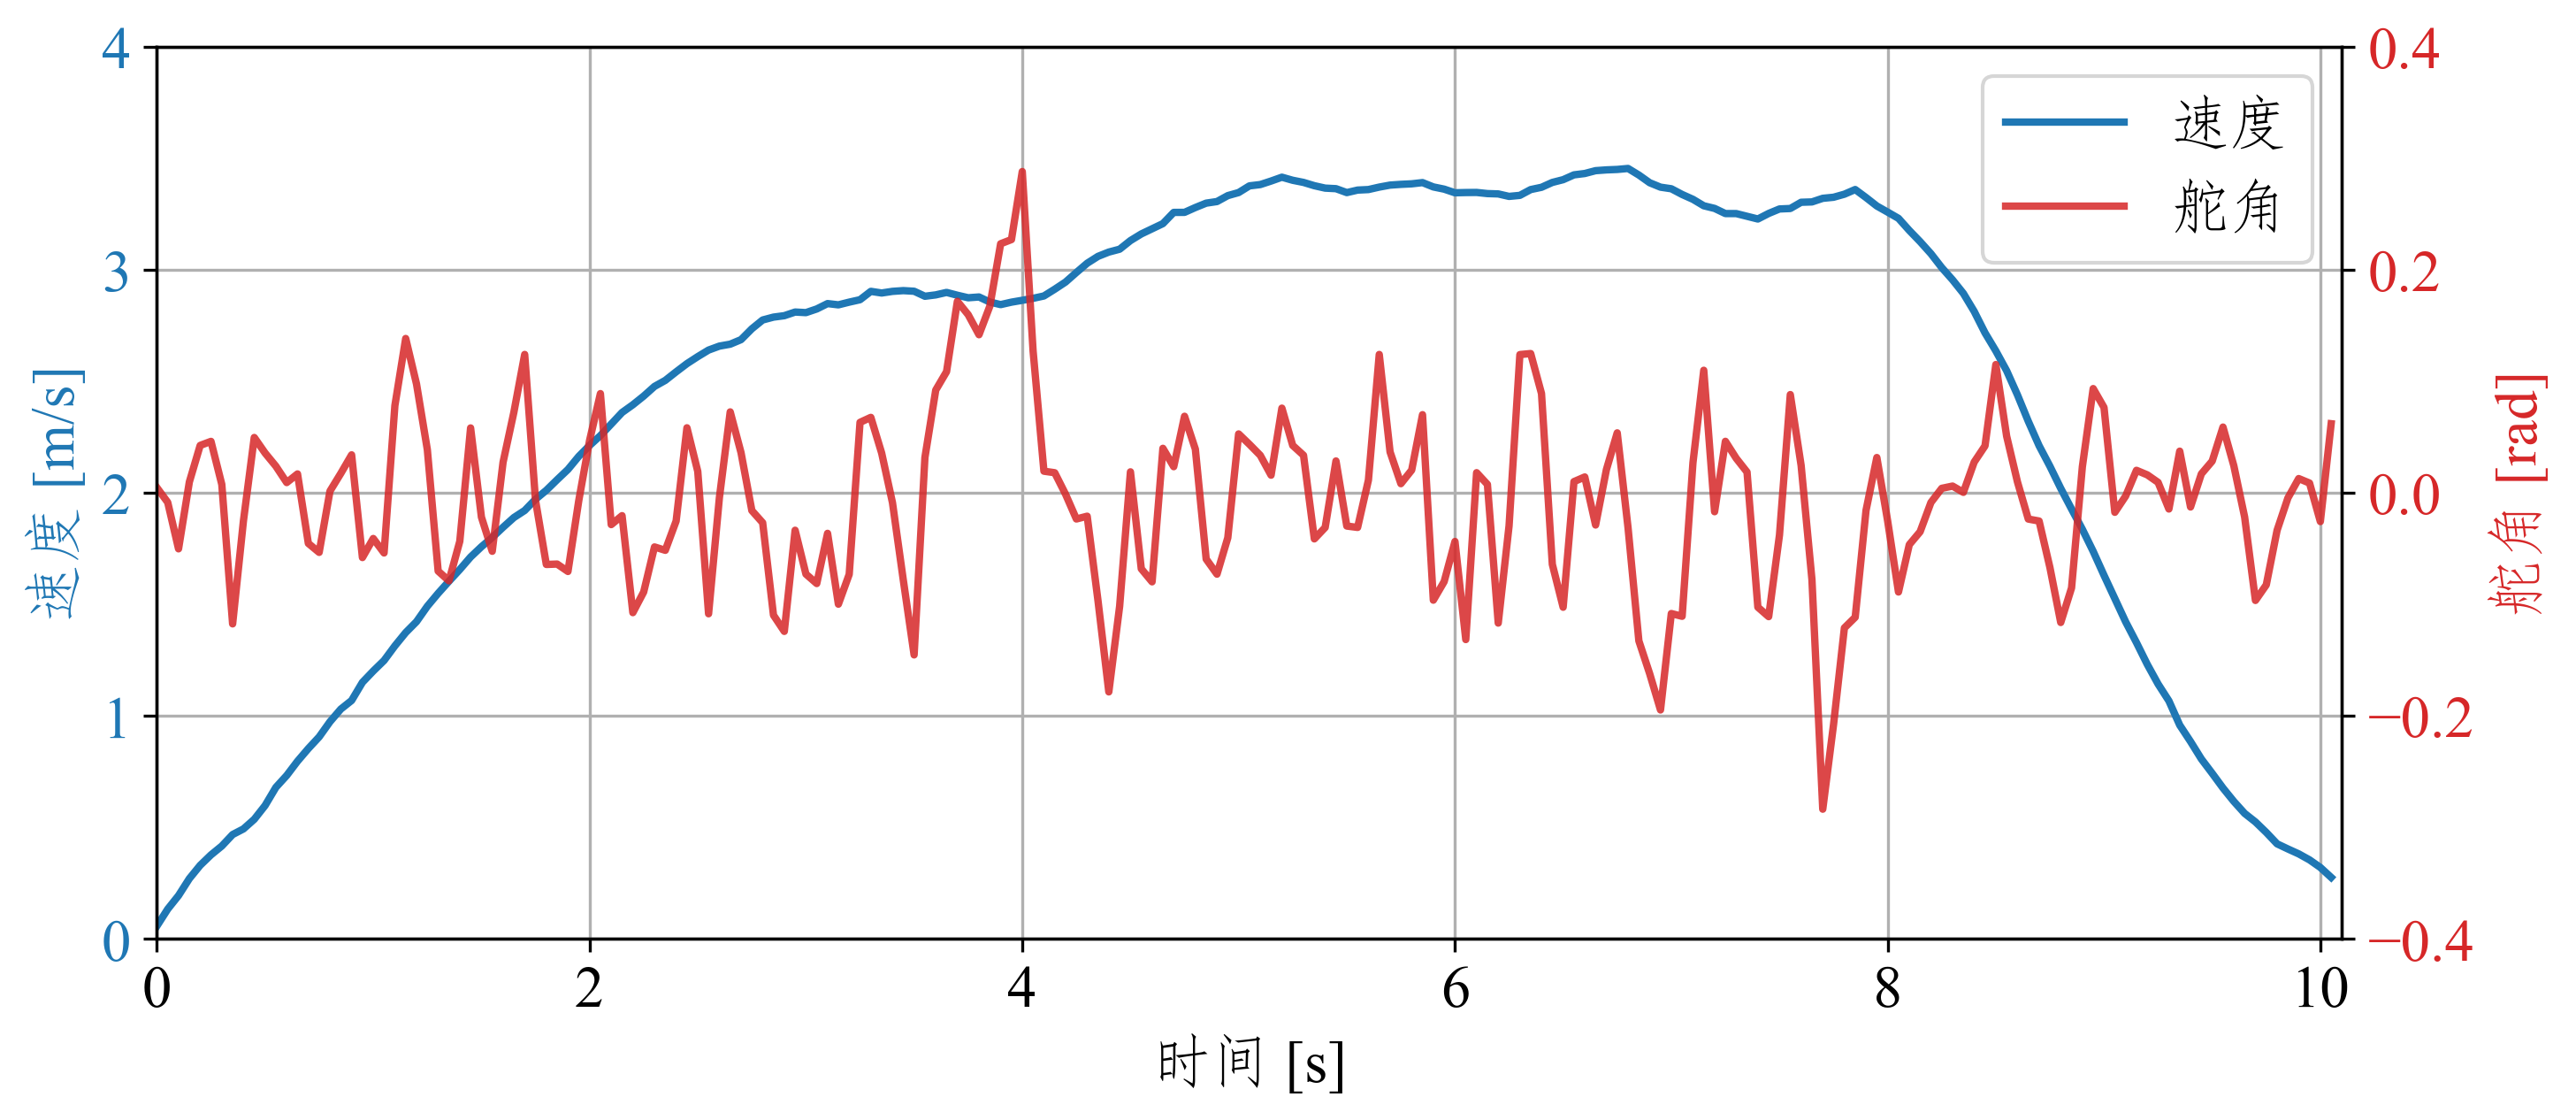
\includegraphics[width=0.33\linewidth]{figure/chapter4/mppi_speed_steering_medium.png}}
    \subfloat[稠密环境中的控制量]{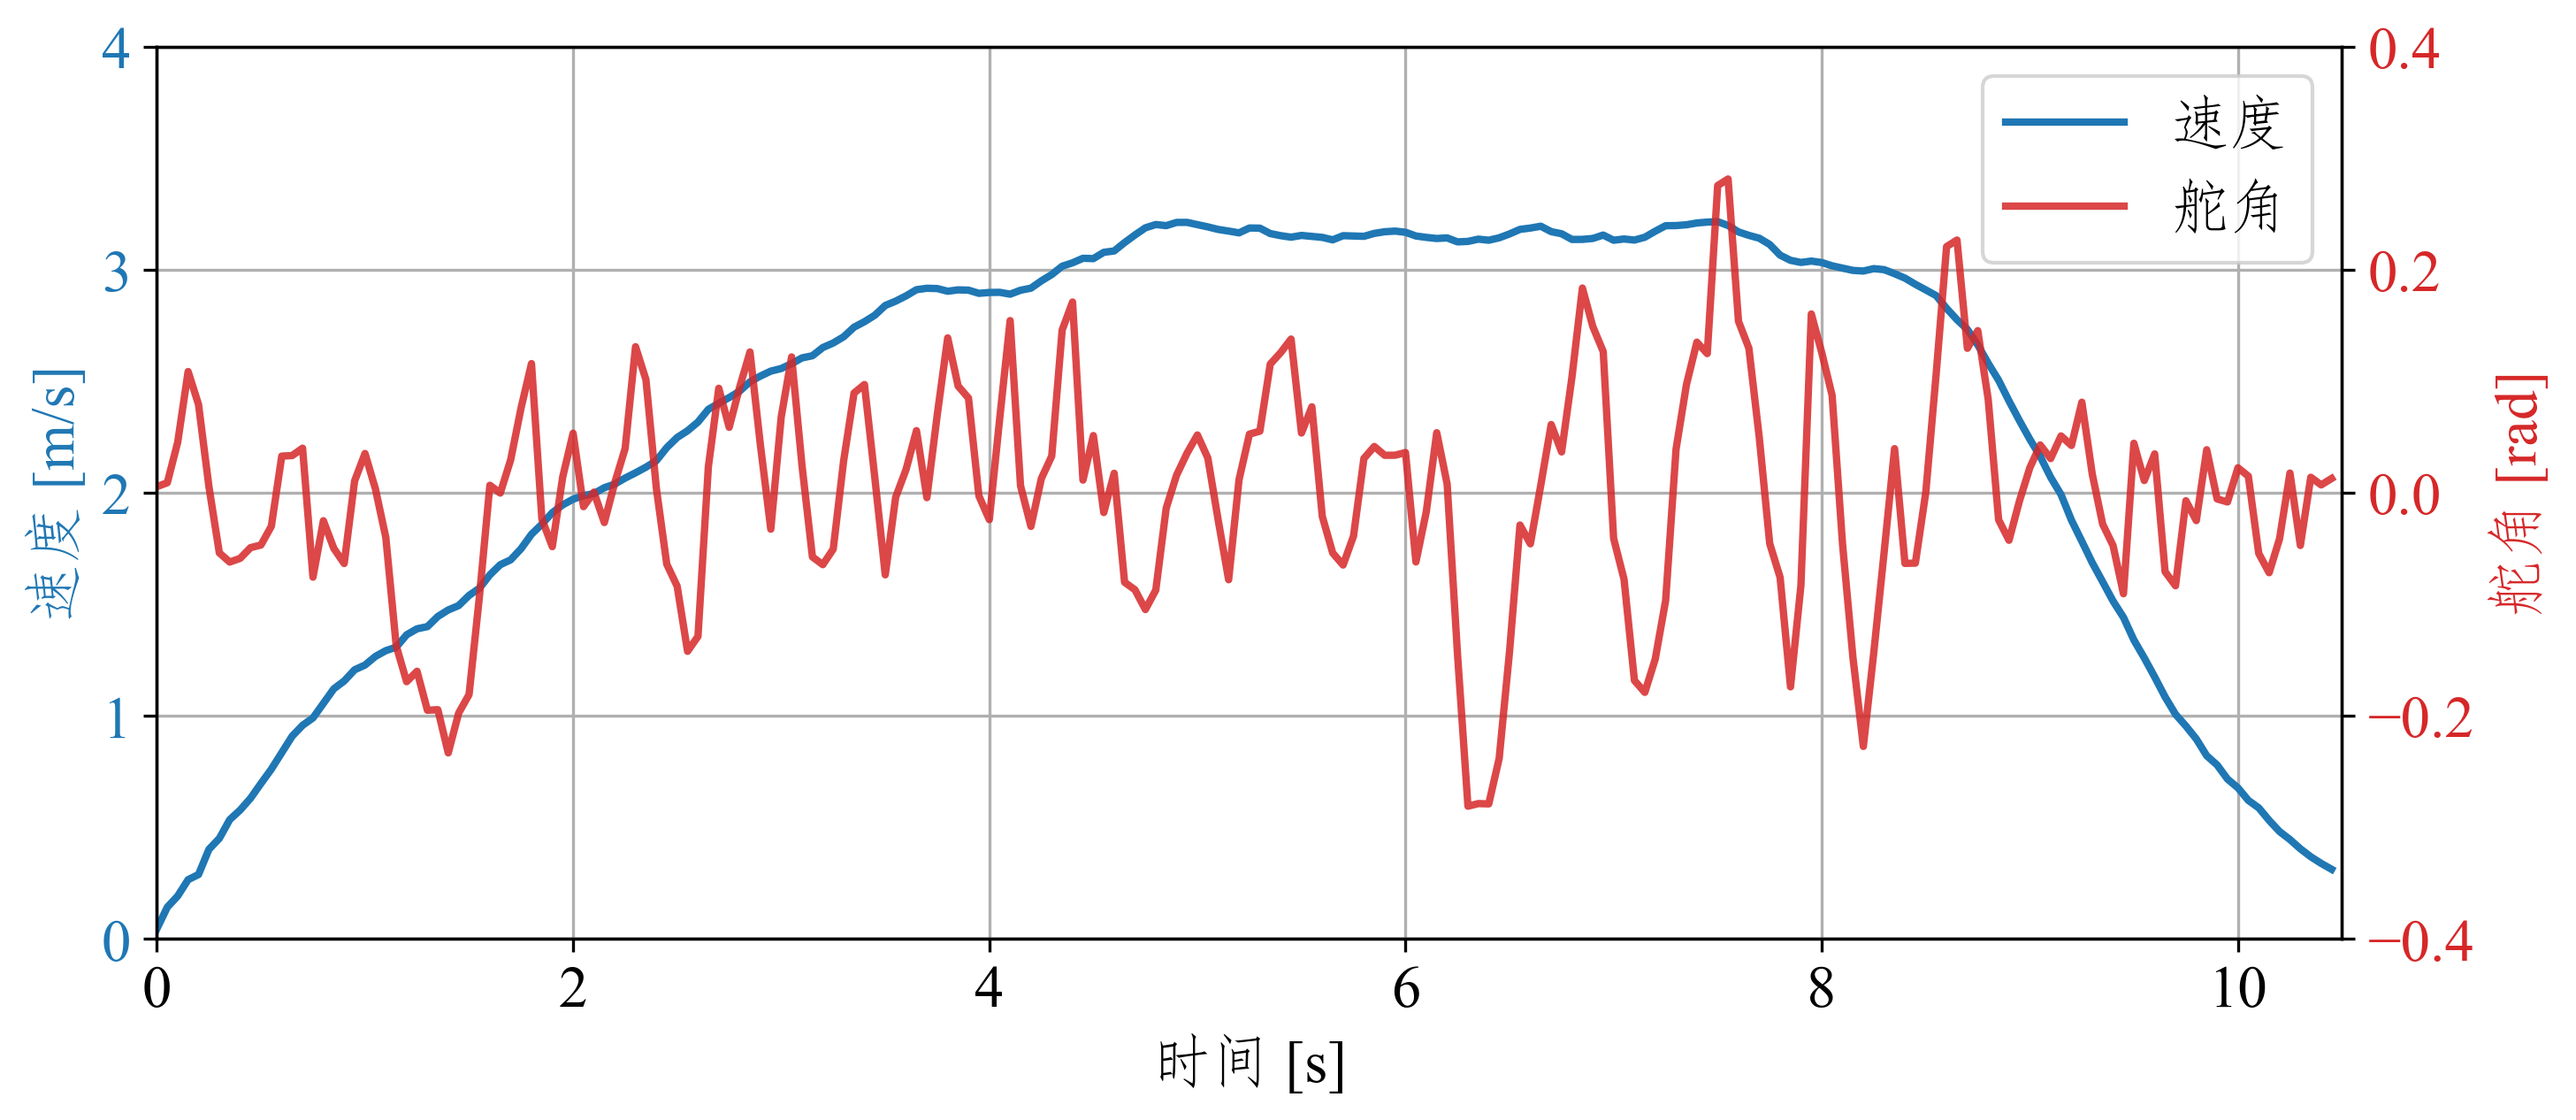
\includegraphics[width=0.33\linewidth]{figure/chapter4/mppi_speed_steering_dense.png}}
    \caption{VPM-MPPI在不同障碍物密度环境中的导航轨迹与控制变化曲线}
    \label{fig:pybullet-traj}
\end{figure}
为了评估VPM-MPPI在不同环境复杂度下的导航性能，本节在PyBullet仿真环境中构建了三个不同障碍物密度的导航场景：稀疏环境（20个障碍物）、中等环境（50个障碍物）和稠密环境（120个障碍物）。每个环境中，机器人需要从起始位置导航到目标位置，同时避开随机分布的障碍物。图\ref{fig:pybullet-traj}展示了VPM-MPPI在不同障碍物密度环境中的导航轨迹与控制变化曲线。可以看出，在稀疏环境中，机器人能够以较高的速度直接朝着目标位置移动，控制输入相对平稳；在中等环境中，机器人需要进行一些路径调整以避开障碍物，控制输入出现了一些波动；而在稠密环境中，机器人需要频繁地调整路径以避开大量的障碍物，控制输入表现出更大的波动。这些结果表明，VPM-MPPI能够适应不同复杂度的环境，并生成合理的导航轨迹和控制策略。

\subsection{消融实验}

\begin{figure}[ht]
    \centering
    \subfloat[$\lambda=0.1$的运行轨迹]{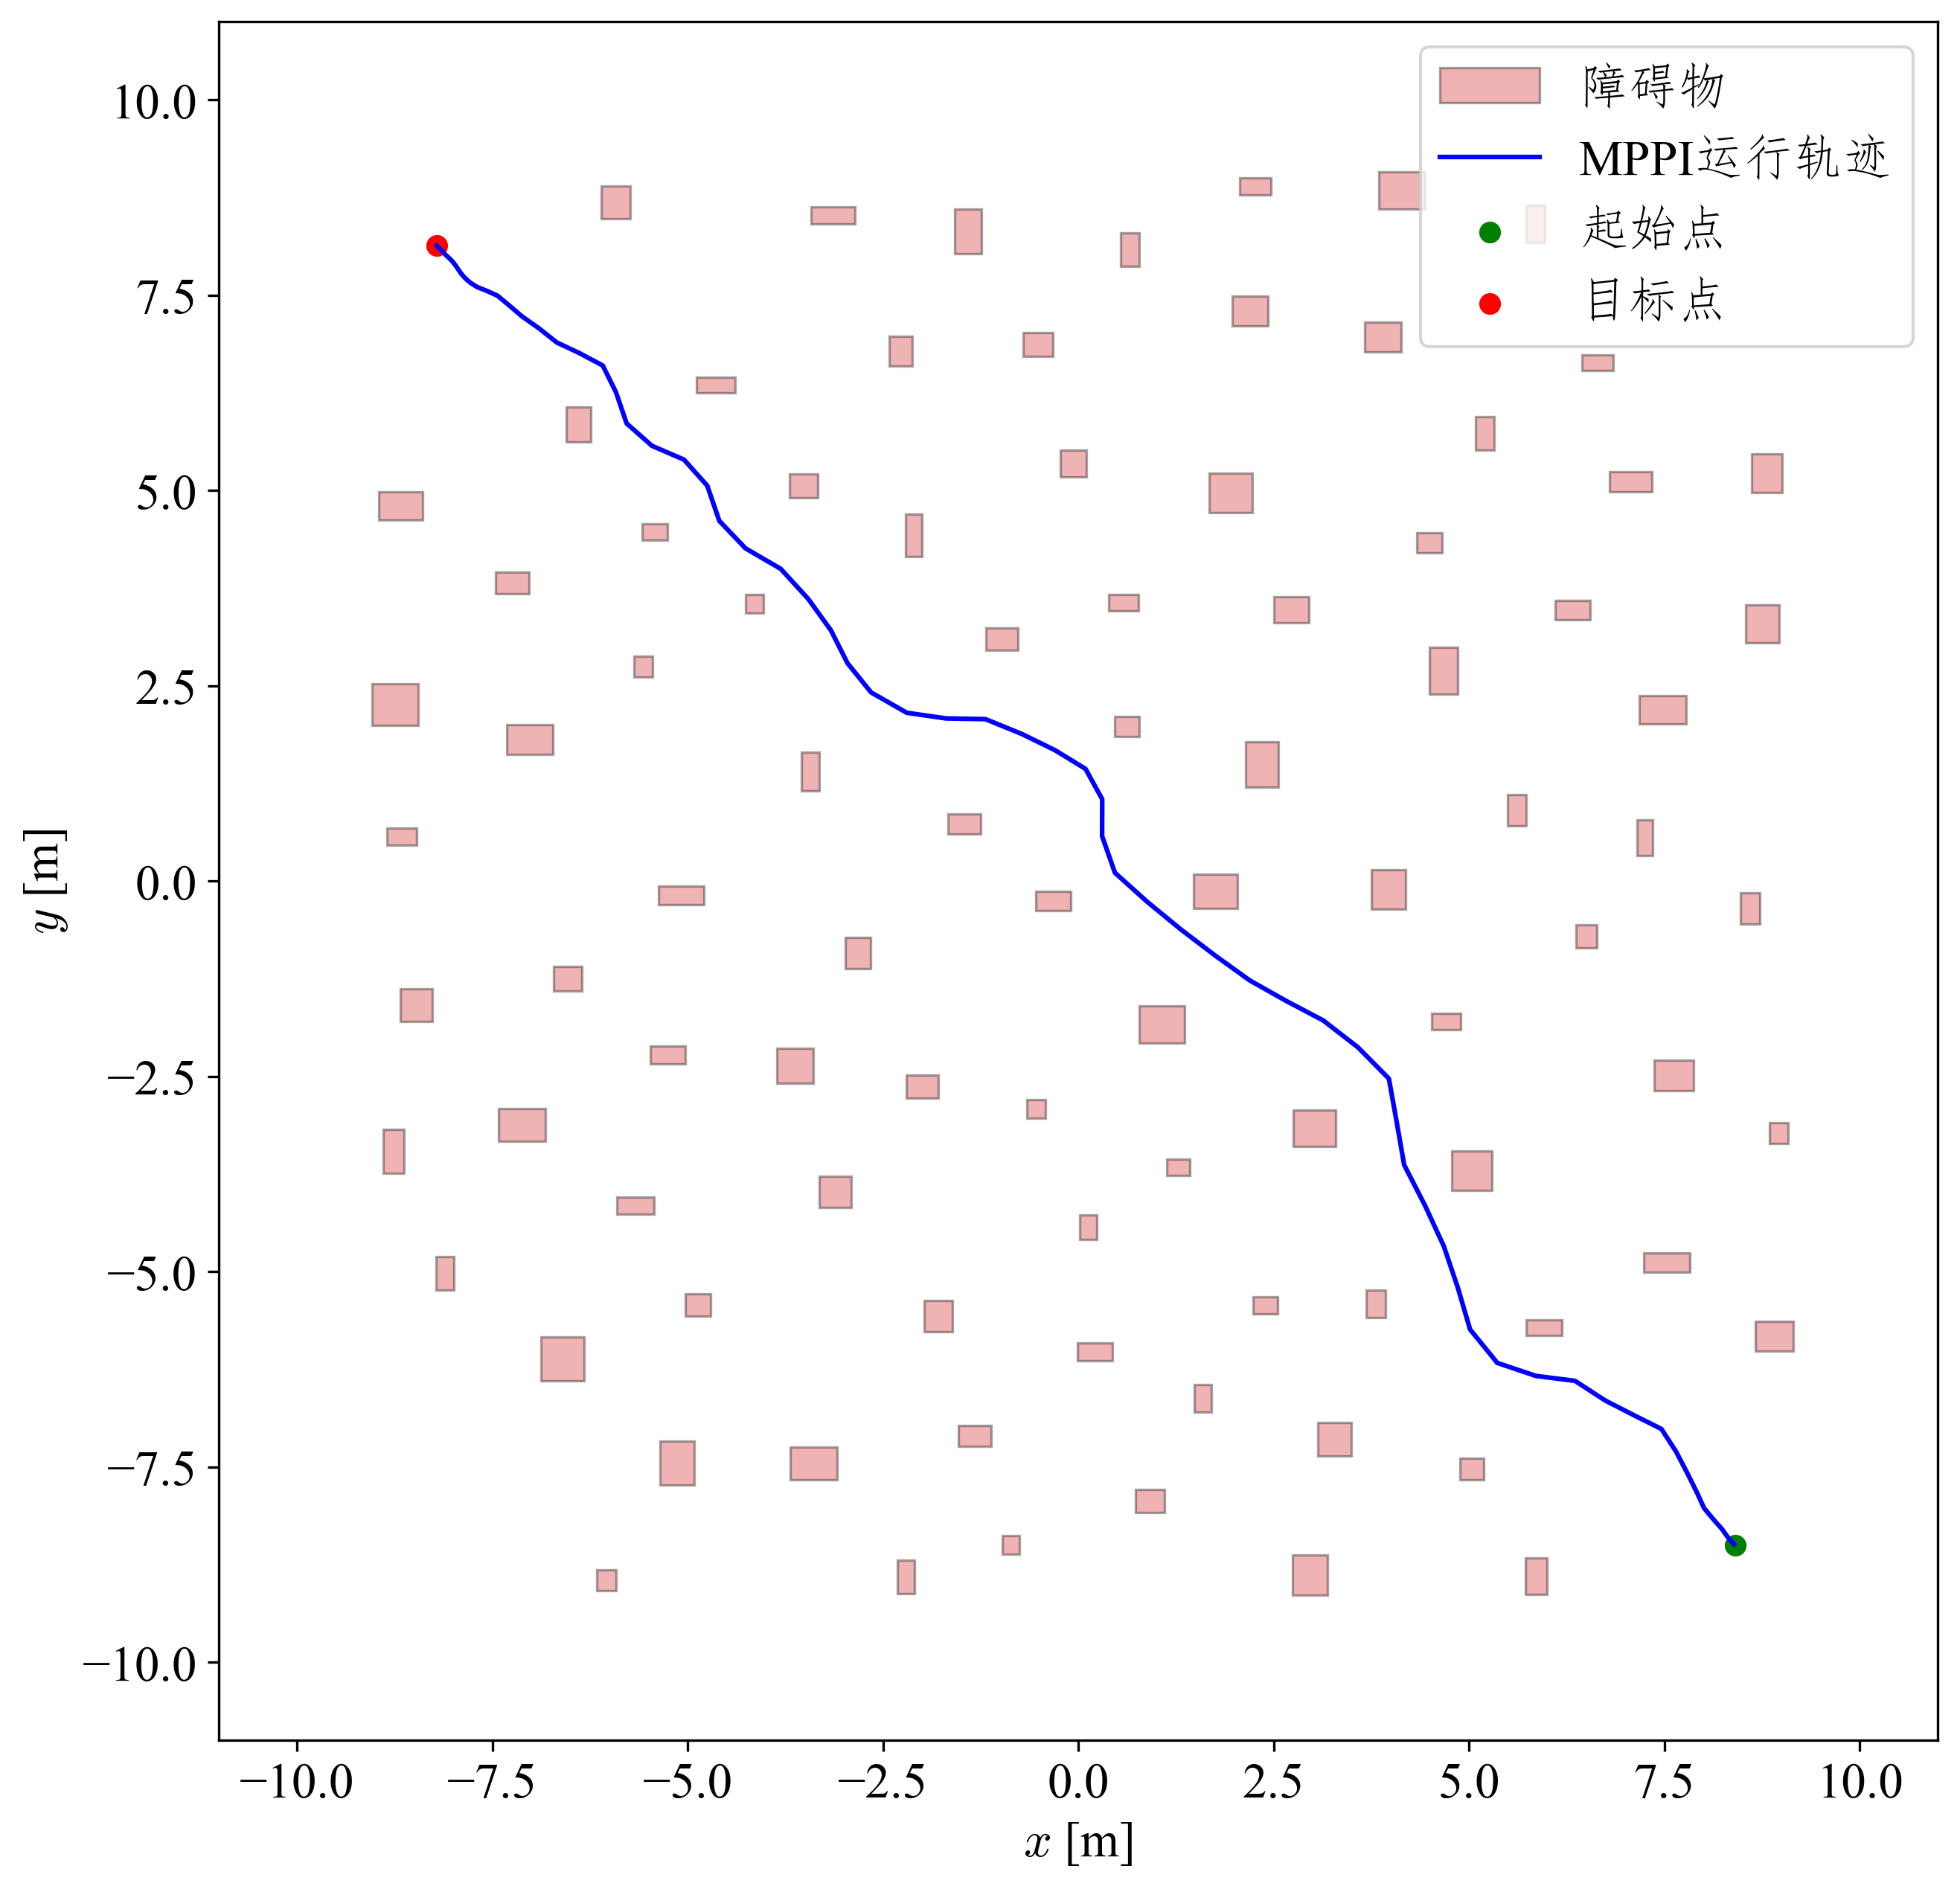
\includegraphics[width=0.33\linewidth]{figure/chapter4/mppi_trajectory_dense_lambda0.1.png}}
    \subfloat[$\lambda=10.0$的运行轨迹]{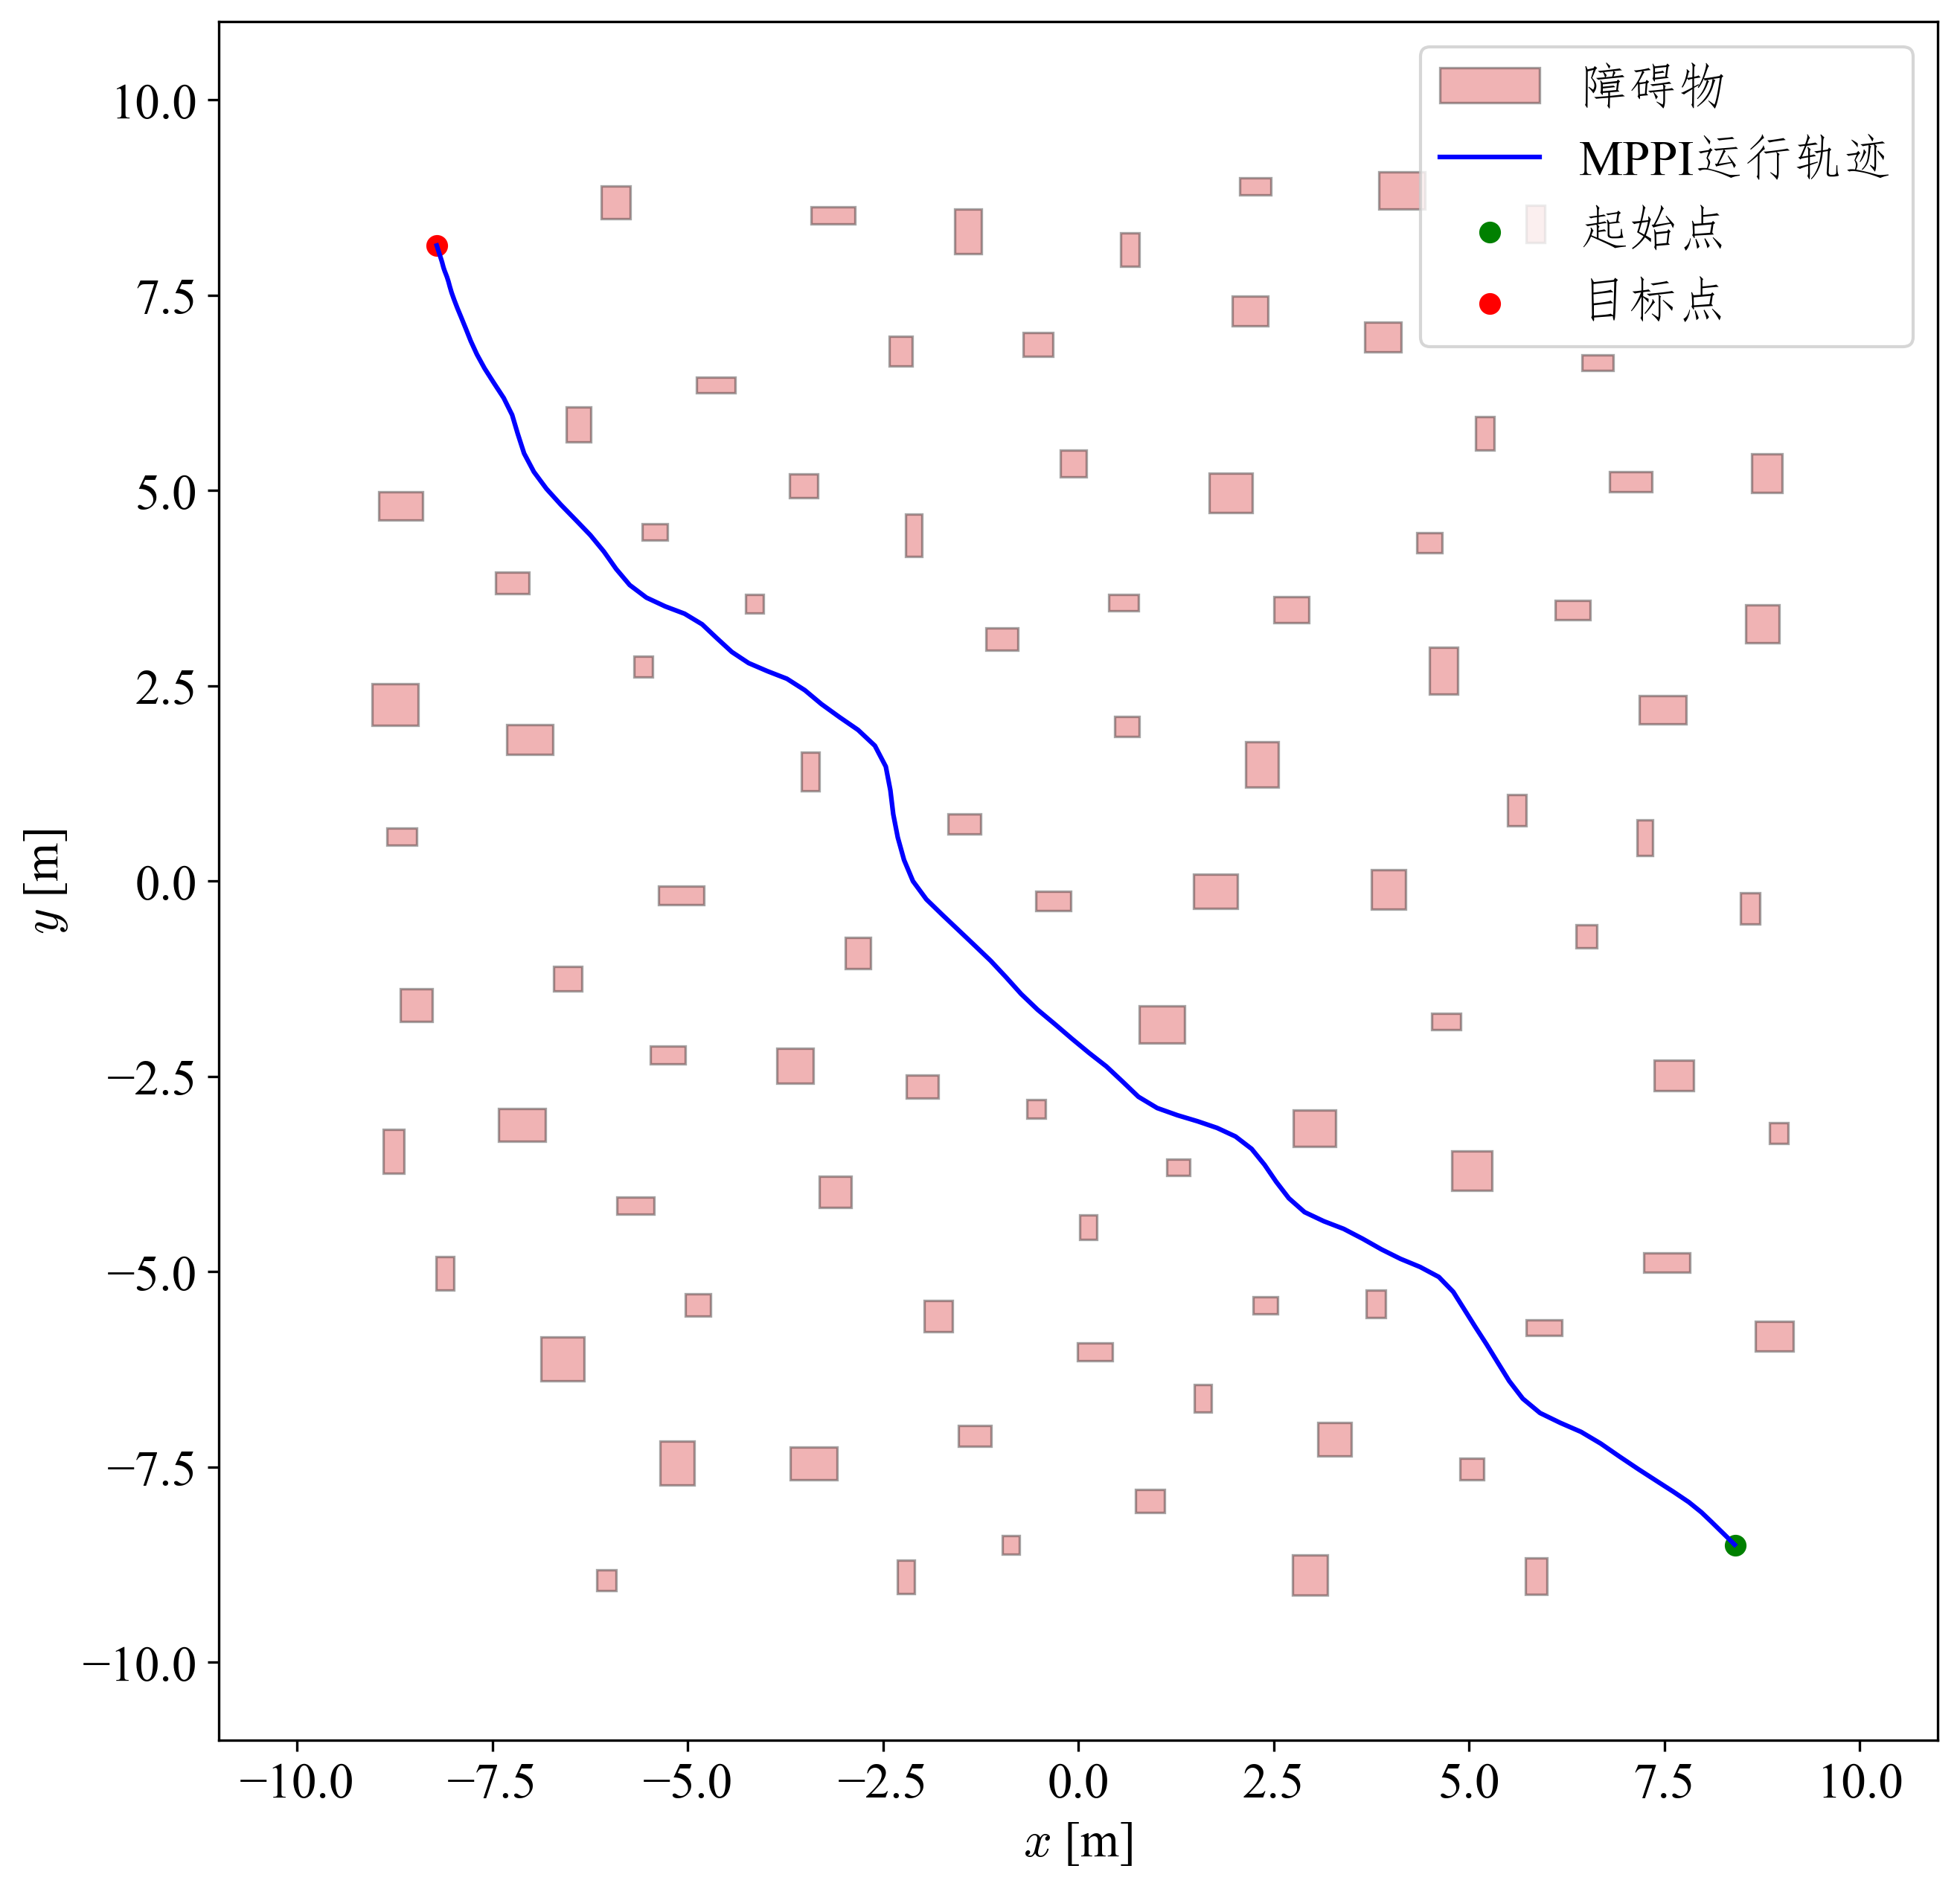
\includegraphics[width=0.33\linewidth]{figure/chapter4/mppi_trajectory_dense_lambda10.png}}
    \subfloat[$\lambda=100.0$的运行轨迹]{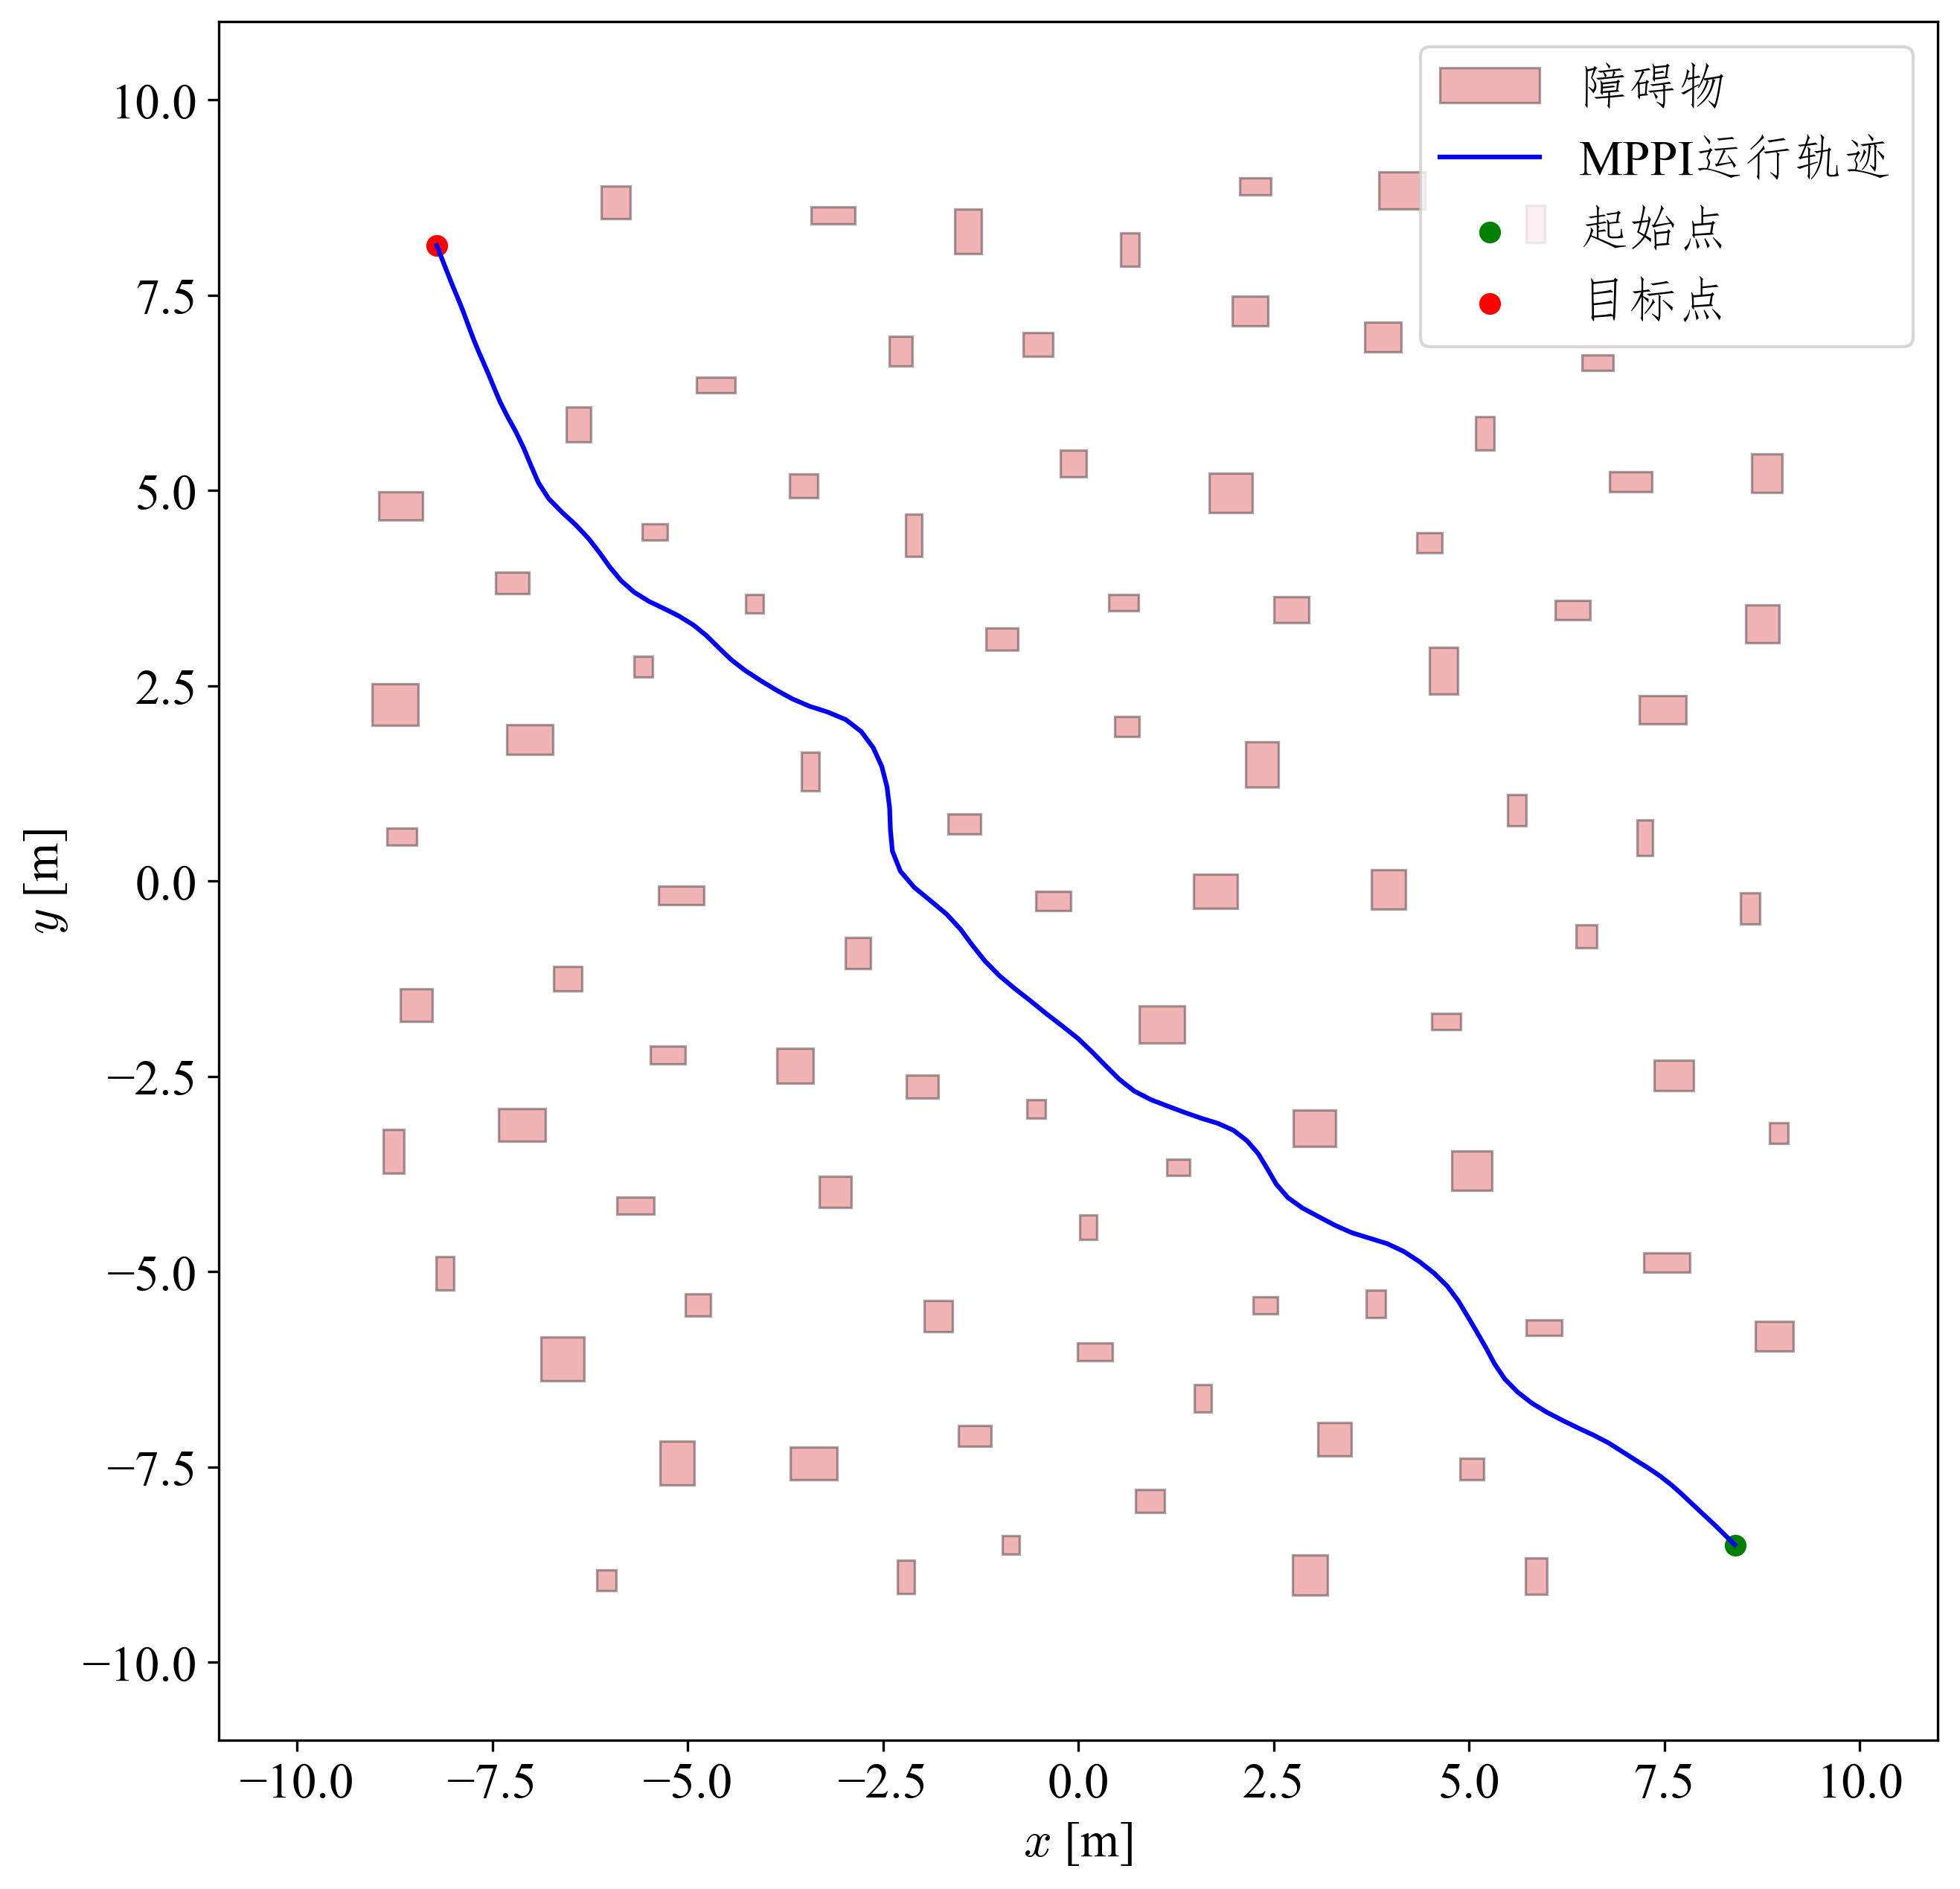
\includegraphics[width=0.33\linewidth]{figure/chapter4/mppi_trajectory_dense_lambda100.png}}

    \subfloat[$\lambda=0.1$的采样轨迹]{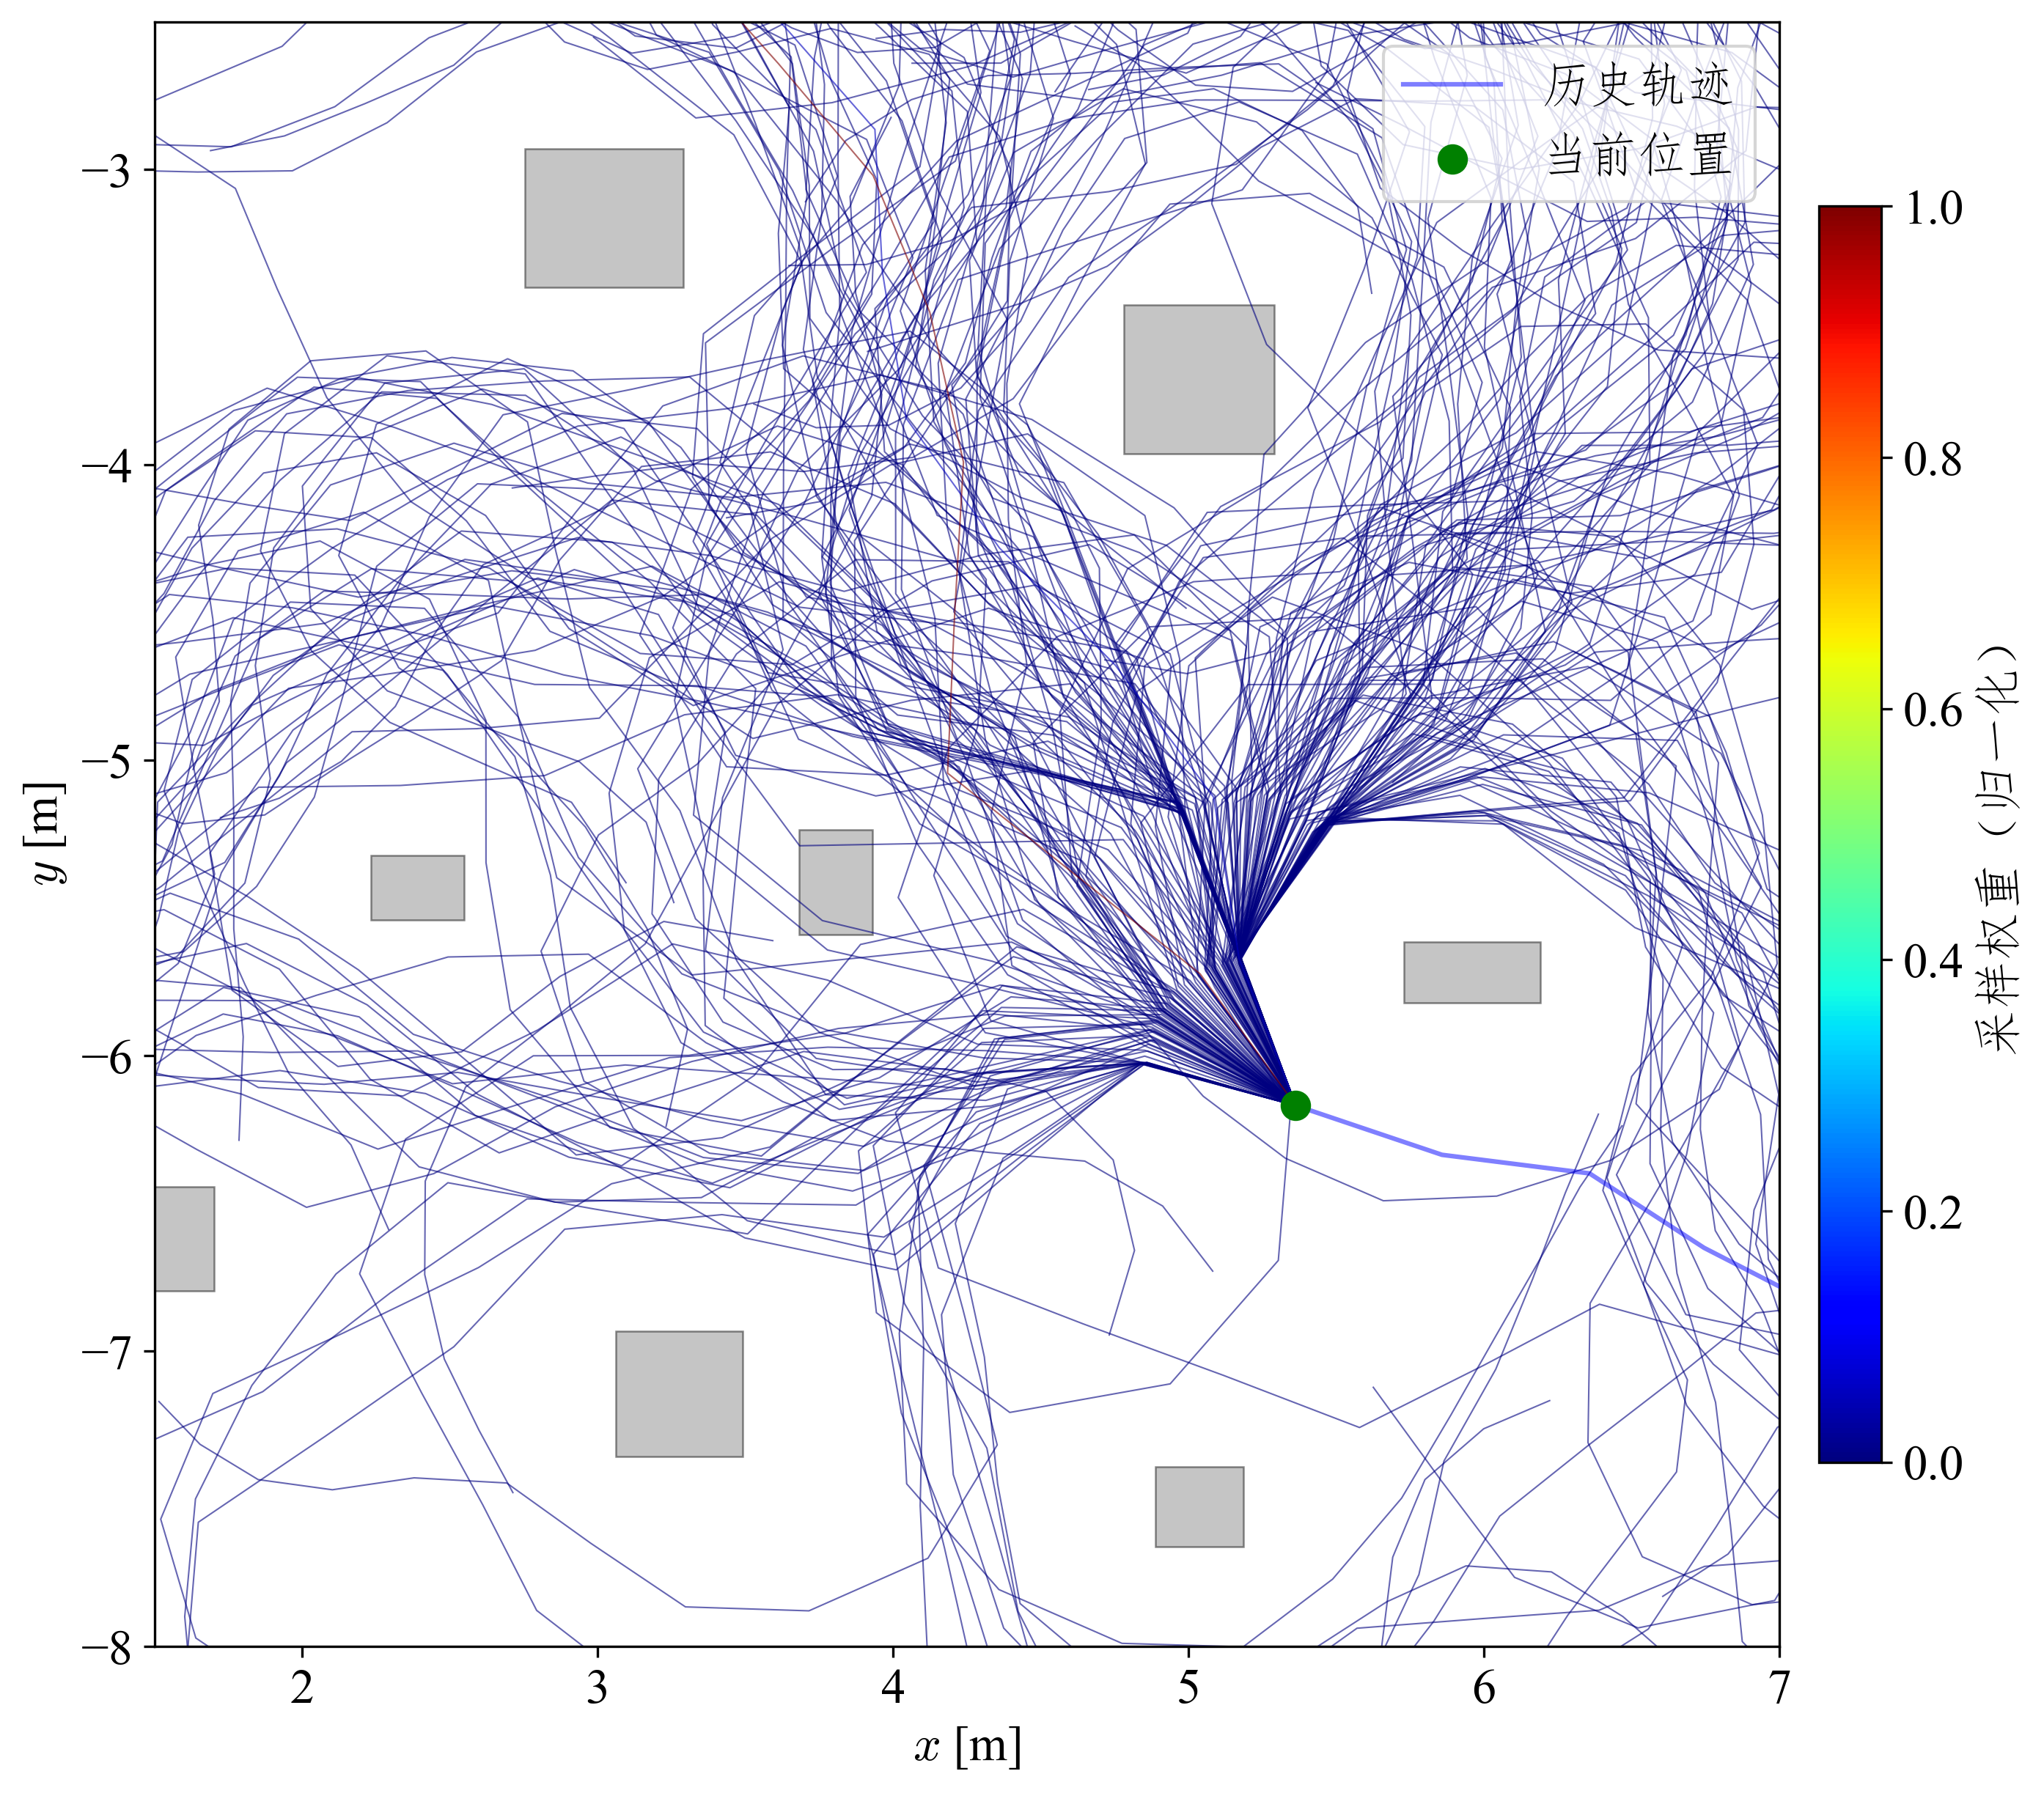
\includegraphics[width=0.33\linewidth]{figure/chapter4/sampled_traj_lambda0.1.png}}
    \subfloat[$\lambda=10.0$的采样轨迹]{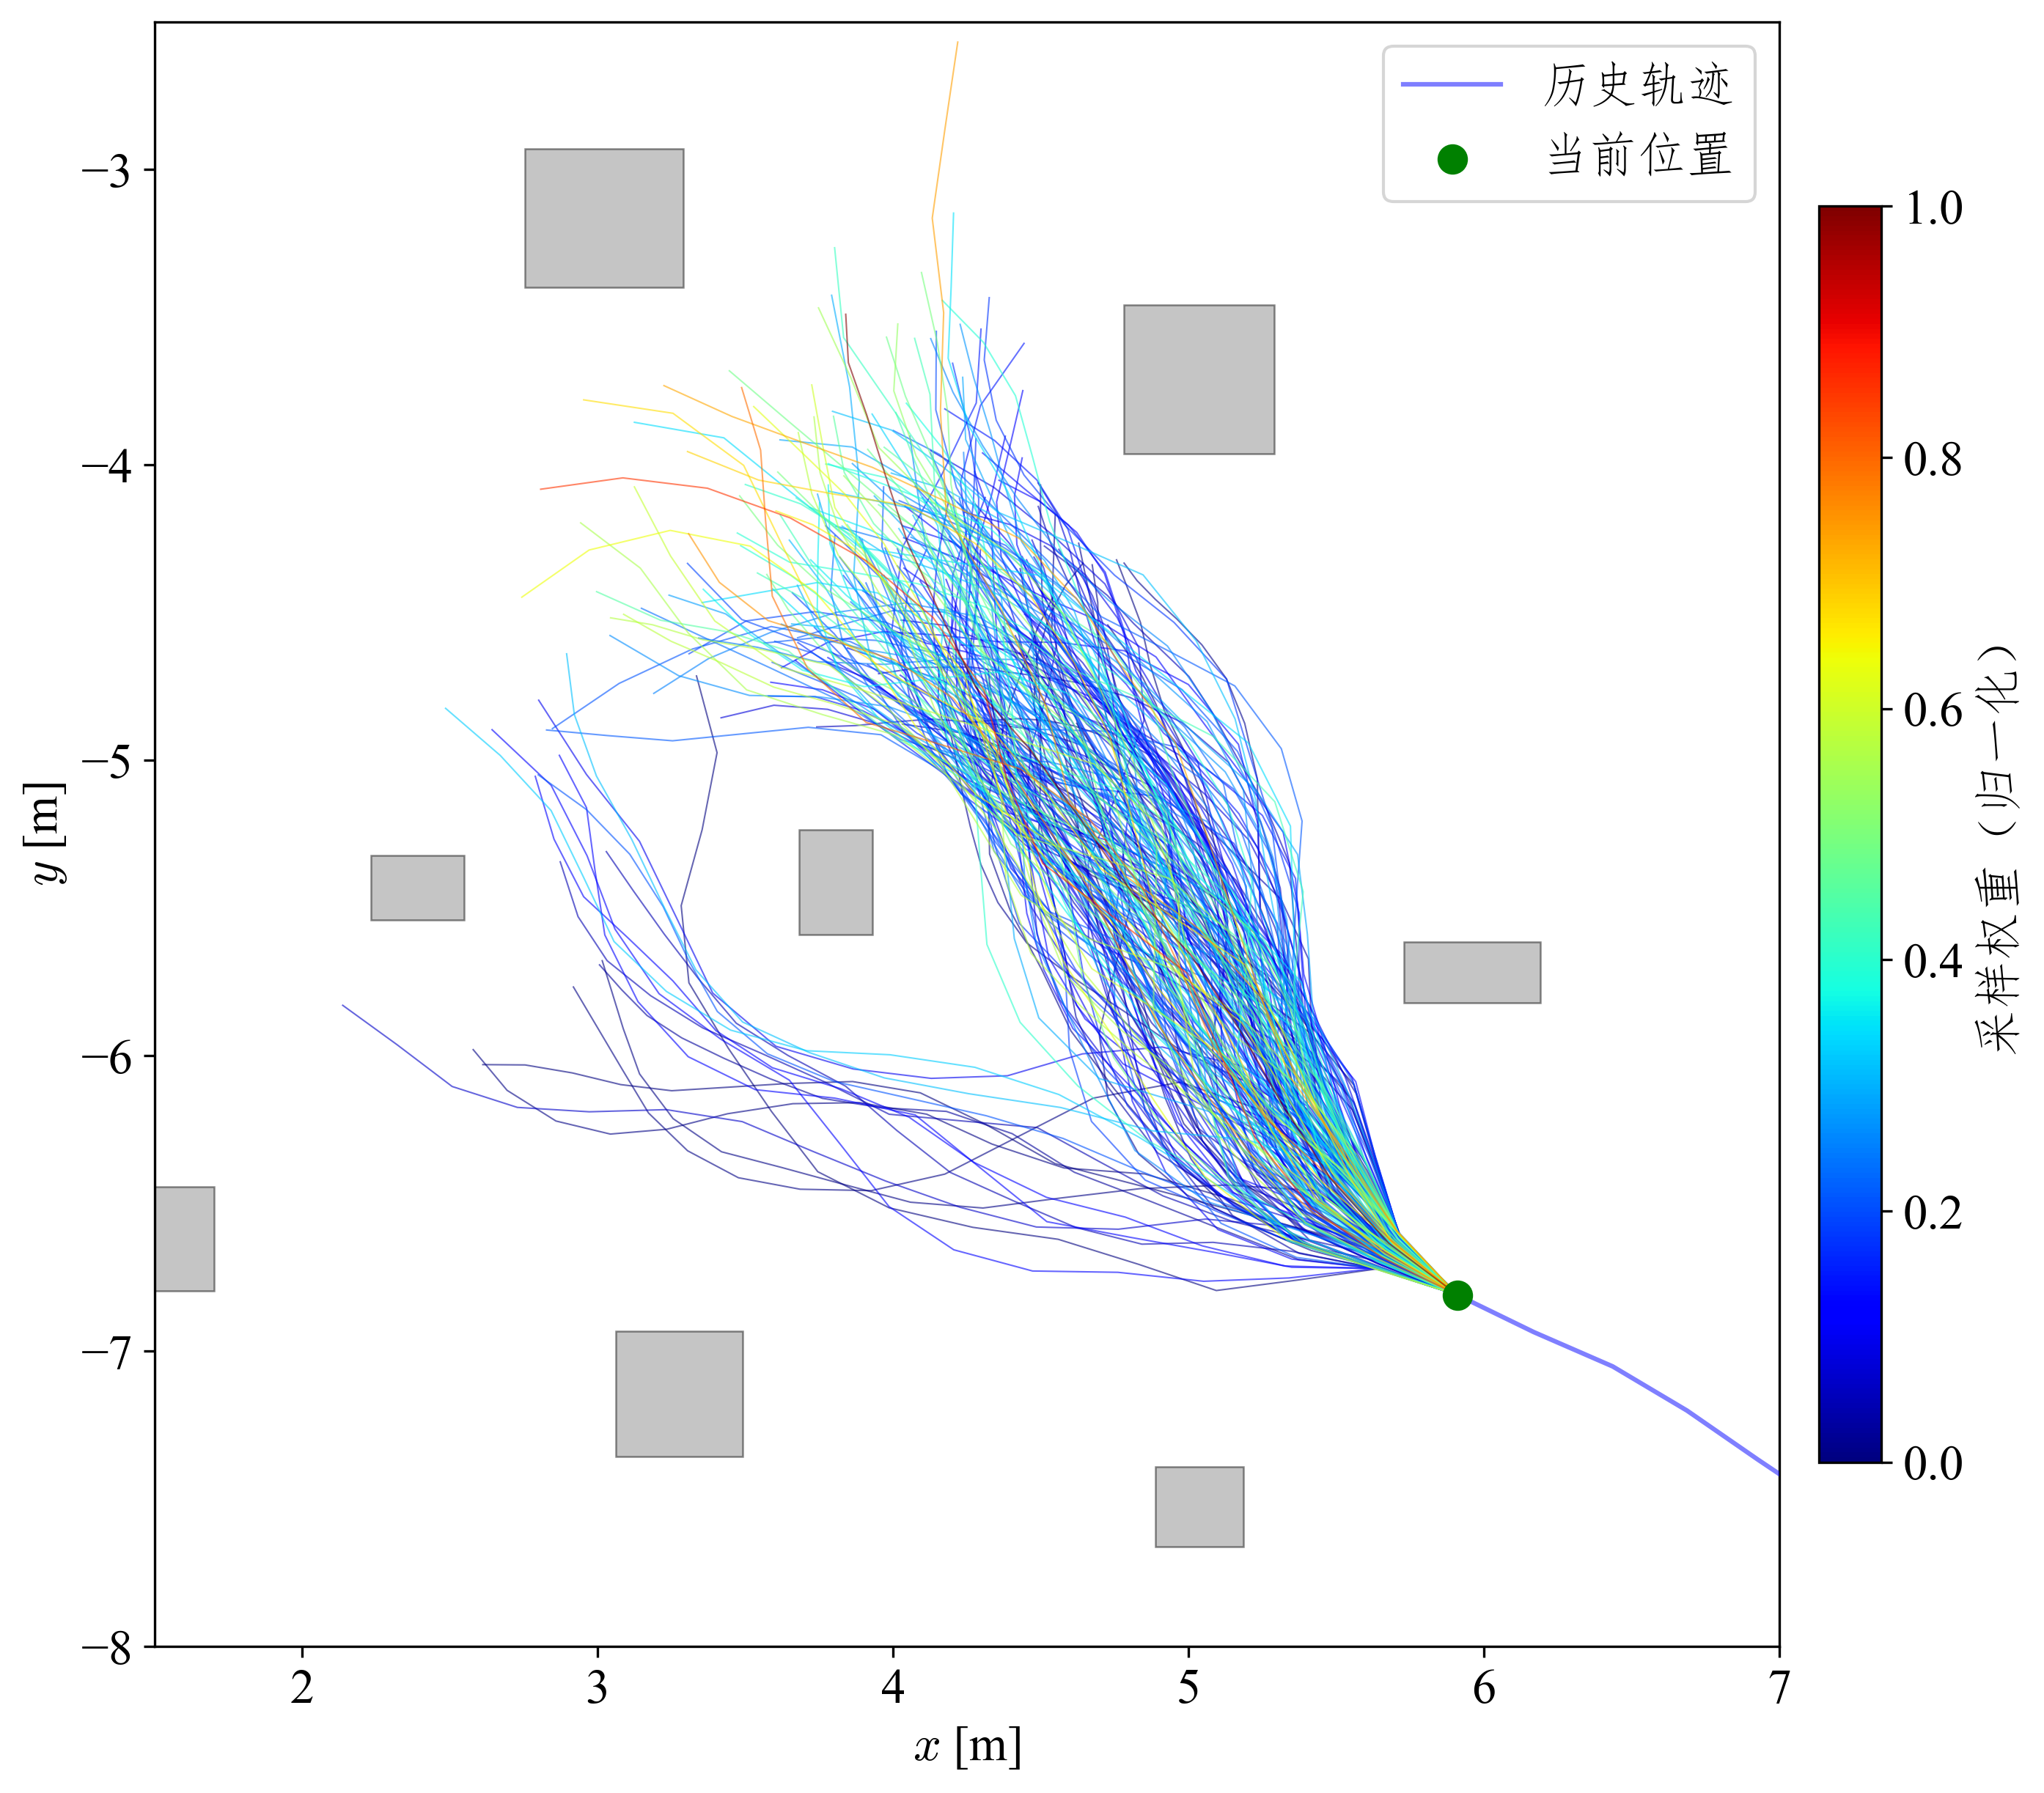
\includegraphics[width=0.33\linewidth]{figure/chapter4/sampled_traj_lambda10.png}}
    \subfloat[$\lambda=100.0$的采样轨迹]{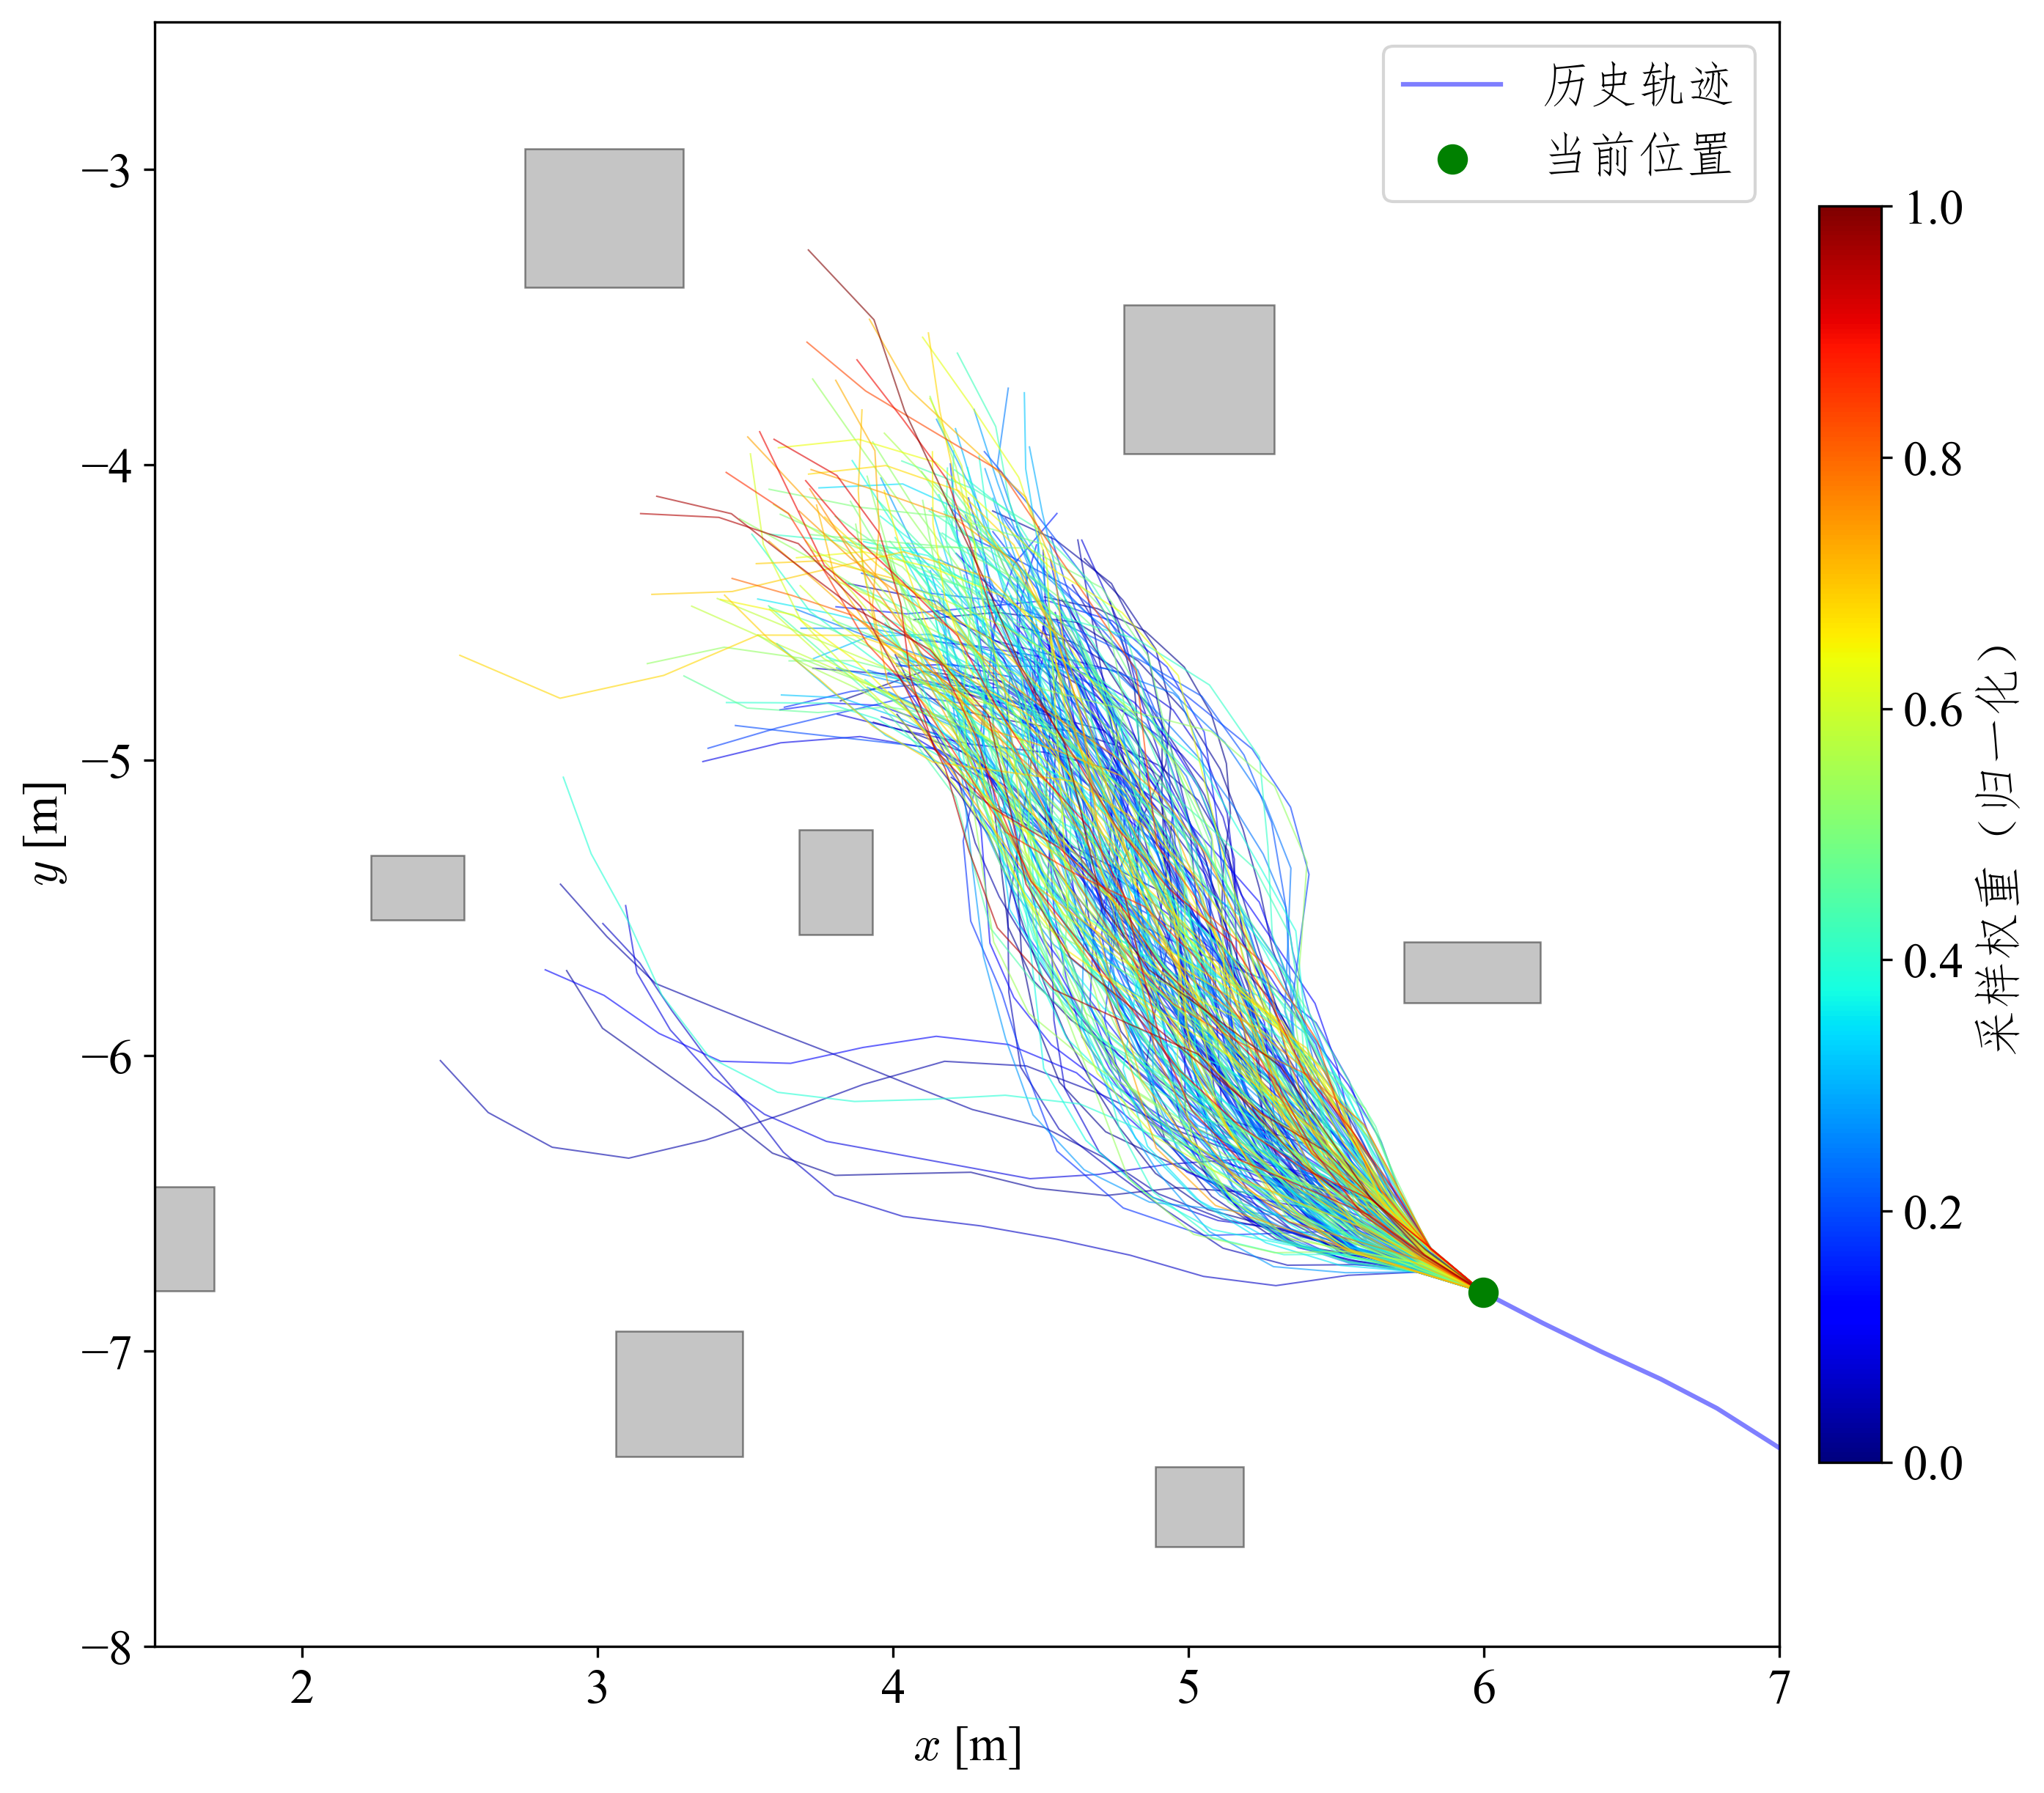
\includegraphics[width=0.33\linewidth]{figure/chapter4/sampled_traj_lambda100.png}}
    \caption{VPM-MPPI在不同$\lambda$值下的导航轨迹与采样轨迹比较}
    \label{fig:lambda-ablation}
\end{figure}
为了分析MPPI算法中温度参数$\lambda$对导航性能的影响，本节在PyBullet仿真环境中的稠密环境下进行了消融实验，分别设置了三个不同的$\lambda$值：$\lambda=0.1$、$\lambda=10.0$和$\lambda=100.0$，并比较了它们在导航任务中的表现。图\ref{fig:lambda-ablation}展示了不同$\lambda$值下的导航轨迹与采样轨迹比较，表\ref{table:lambda-ablation}给出了具体的导航性能比较。可以看出，当$\lambda=0.1$时，控制策略进行大量采样但只聚焦于低成本路径，导致轨迹并不平滑；当$\lambda=100.0$时，控制策略给所有采样路径赋予相似的权重，可能导致优化出的轨迹有一定的不安全性；而当$\lambda=10.0$时，控制策略能够较好地平衡探索和利用，生成了更合理的导航轨迹。这些结果表明，温度参数$\lambda$的选择对于MPPI算法的性能有重要影响，需要根据具体的任务需求进行调整。
\begin{table}[ht]
\renewcommand{\arraystretch}{1.2}
\caption{VPM-MPPI在不同$\lambda$值下的导航性能比较}
\centering
\setlength{\tabcolsep}{20pt}{
    \begin{tabular}{c|ccc}
    \toprule[2pt]
    $\lambda$取值 & SR[\%] & PL[$m$] & AT[$s$]\\
    \midrule[1pt]
    $0.1$ & $90.0$ & $26.97\pm0.54$ & $8.83\pm0.26$ \\
    $10.0$ & $100.0$ & $24.27\pm0.17$ & $10.87\pm0.15$ \\
    $100.0$ & $85.0$ & $24.23\pm0.14$ & $12.70\pm0.12$ \\
    \bottomrule[2pt]
\end{tabular}}
\label{table:lambda-ablation}
\end{table}

\begin{figure}[ht]
    \centering
    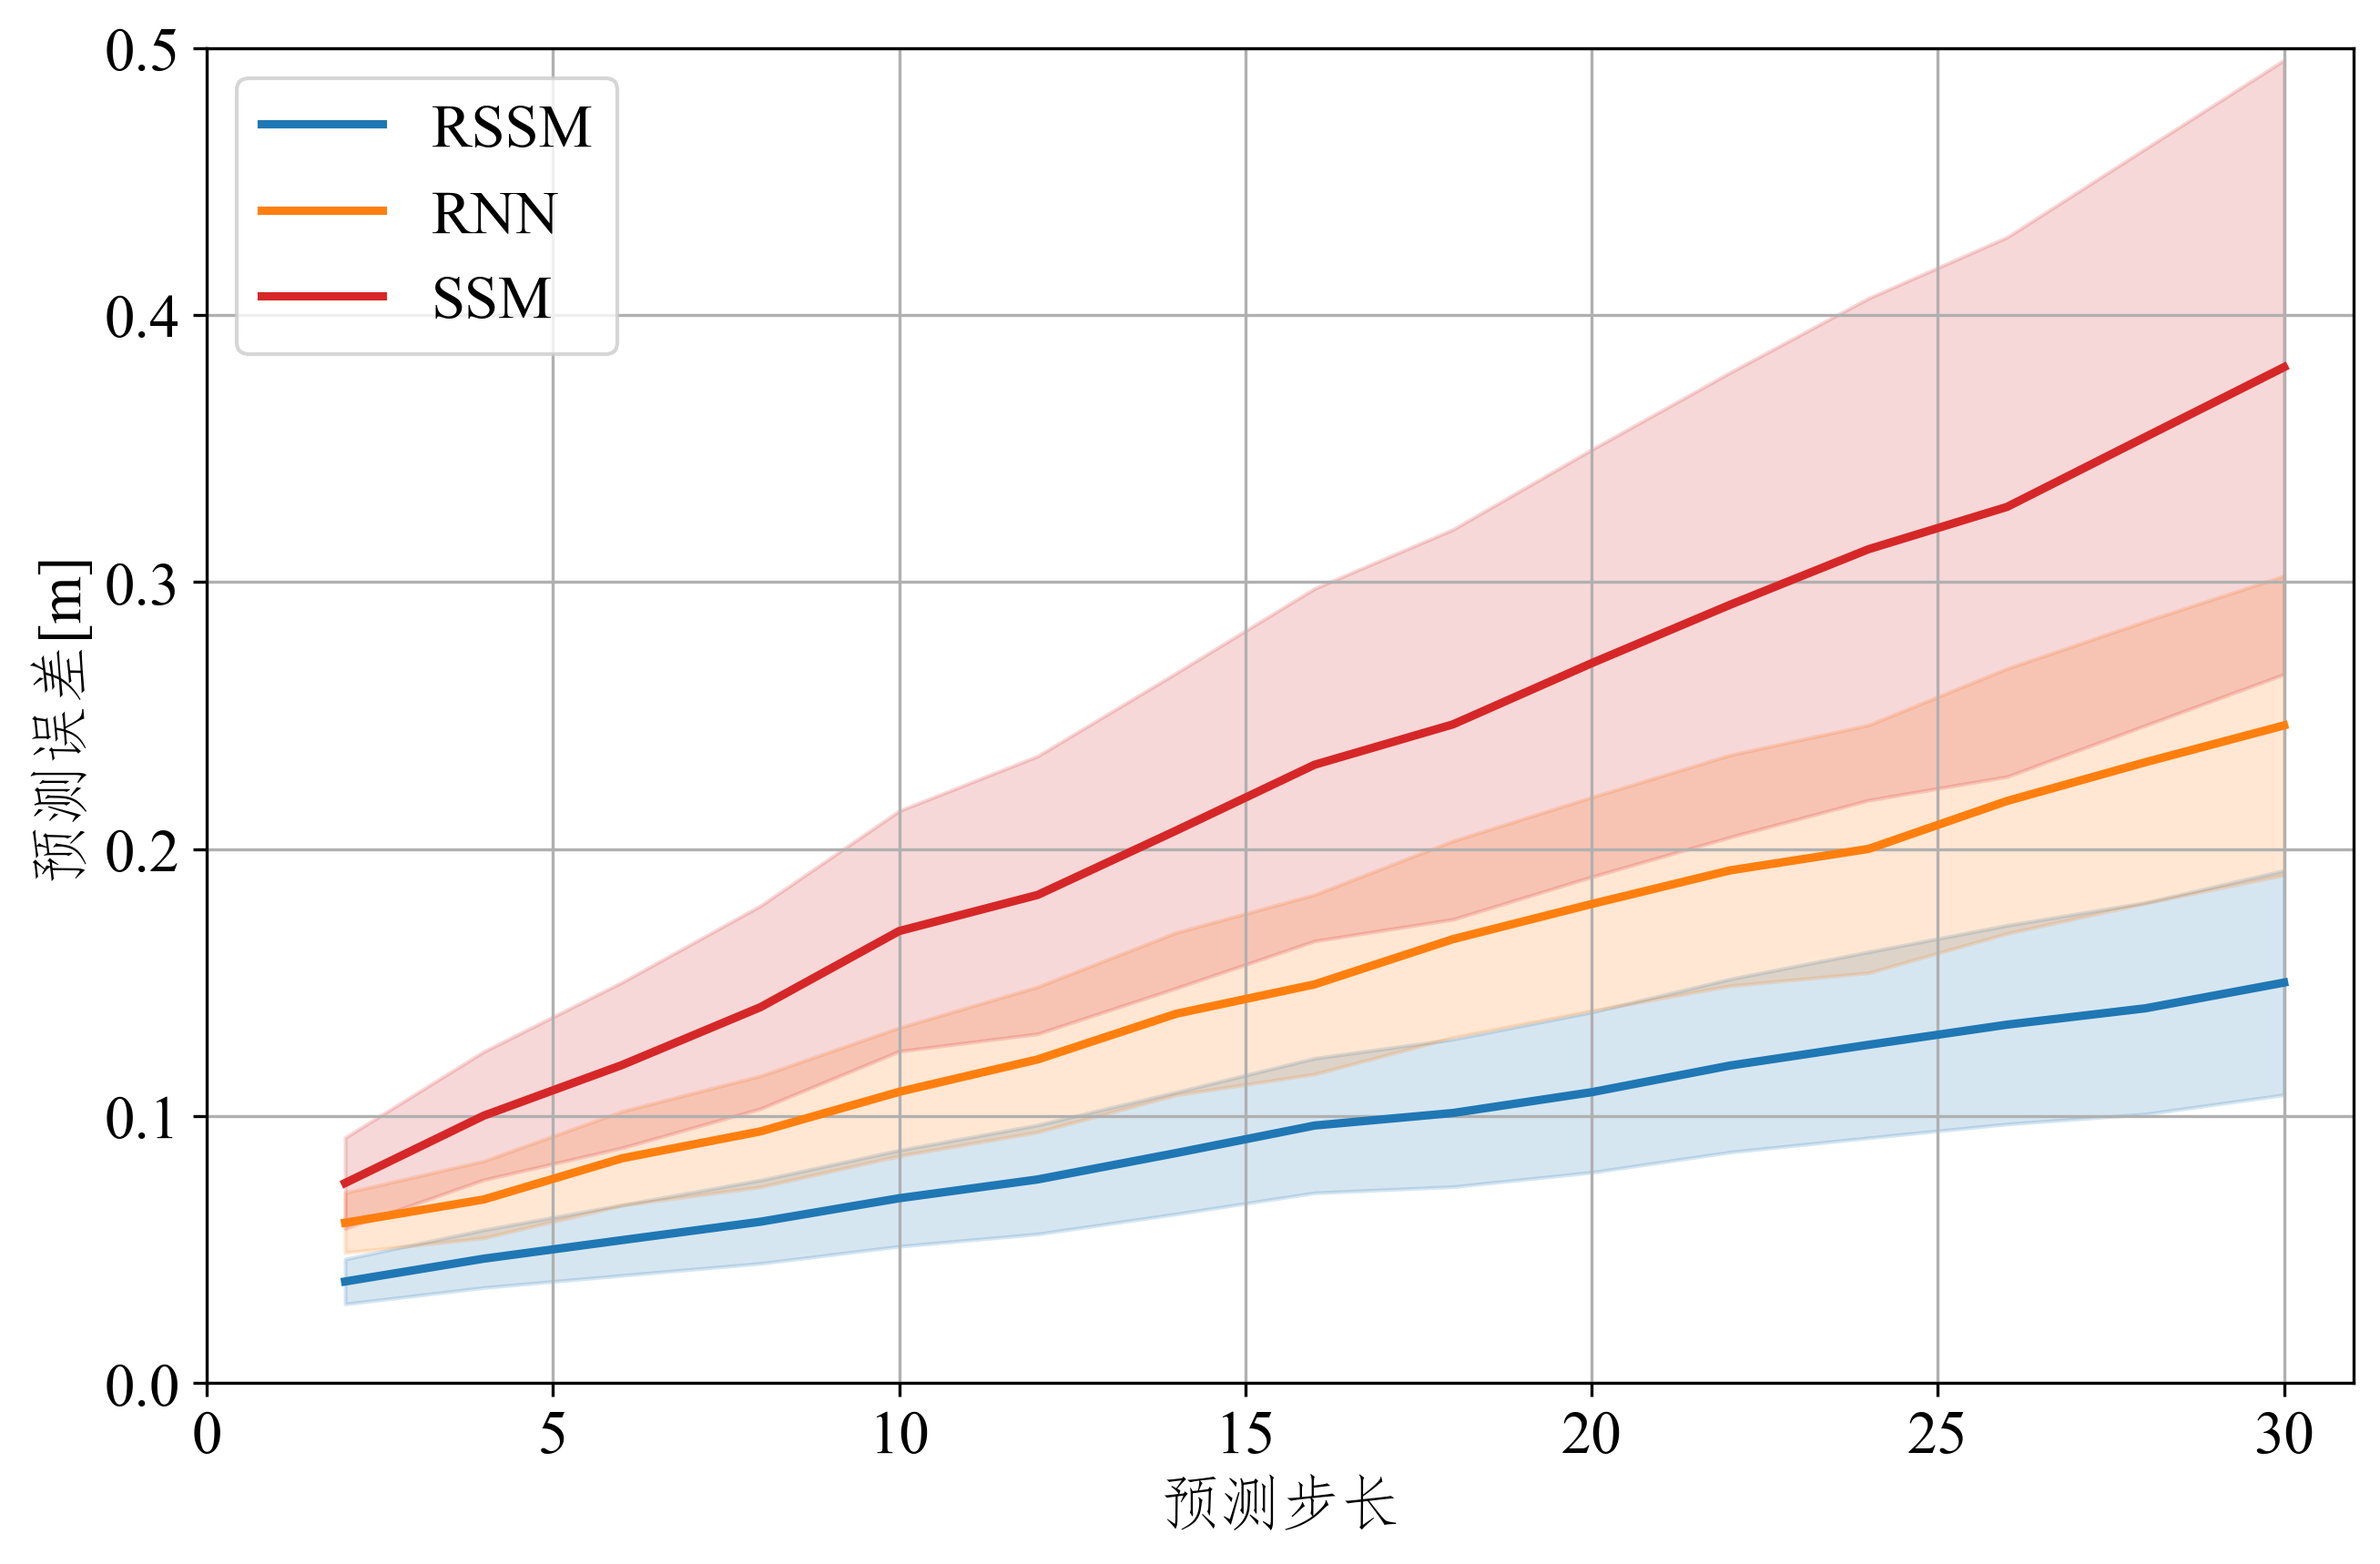
\includegraphics[width=0.6\textwidth]{figure/chapter4/prediction_error_vs_horizon.png}
    \caption{不同模型的预测误差随预测步长的变化曲线}
    \label{fig:prediction-error}
\end{figure}
为了评估VPM的预测性能，本节使用了相同的轨迹数据训练了三种不同的预测模型：本文提出的循环状态空间模型（RSSM）、传统的状态空间模型（SSM）和只使用RNN的预测模型（RNN）。然后在测试集轨迹上记录了每个模型的预测误差随预测步长的变化曲线，如图\ref{fig:prediction-error}所示。可以看出，本文提出的RSSM模型的预测误差明显低于传统的SSM模型和只使用RNN的模型。这表明，确定性循环状态和随机性状态的结合能够更准确地捕捉环境的动态变化，提供更准确的预测结果。然而，我们发现，随着预测步长的增加，所有模型的预测误差都有所增加。因此在MPPI算法中，选择一个合适的预测时域长度非常重要，有助于在预测准确性和控制性能之间进行权衡。

\begin{table}[ht]
\renewcommand{\arraystretch}{1.2}
\caption{VPM-MPPI在不同预测步长下的导航性能比较}
\centering
\setlength{\tabcolsep}{20pt}{
    \begin{tabular}{c|ccc}
    \toprule[2pt]
    预测步长 & SR[\%] & PL[$m$] & AT[$s$]\\
    \midrule[1pt]
    $5$ & $100.0$ & $26.58\pm0.29$ & $12.57\pm0.26$ \\
    $10$ & $100.0$ & $24.74\pm0.16$ & $11.44\pm0.19$ \\
    $15$ & $100.0$ & $24.27\pm0.17$ & $10.87\pm0.15$ \\
    $20$ & $95.0$ & $24.04\pm0.21$ & $10.49\pm0.24$ \\
    $25$ & $87.5$ & $23.89\pm0.25$ & $10.24\pm0.27$ \\
    \bottomrule[2pt]
\end{tabular}}
\label{table:prediction-horizon-ablation}
\end{table}
针对预测步长对导航性能的影响，本节在稠密障碍物环境下进行了消融实验，分别设置了五个不同的预测步长：5、10、15、20和25，并比较了它们在导航任务中的表现。表\ref{table:prediction-horizon-ablation}展示了不同预测步长下的导航性能比较结果。可以看出，当预测步长为$15$时，导航性能达到了最佳水平，成功率为100\%，平均路径长度和平均到达时间也表现出了较好的结果。当预测步长过短时，控制器生成了较为短视的策略，虽然成功率仍然很高，但平均路径长度和平均到达时间较长；当预测步长过长时，成功率略微下降，但平均路径长度和平均到达时间有所改善，可能是由于更长的预测时域提供了更多的未来信息，但预测误差积累削弱了闭环控制的鲁棒性。

\begin{figure}[ht]
    \centering
    \subfloat[本文奖励函数的运行轨迹]{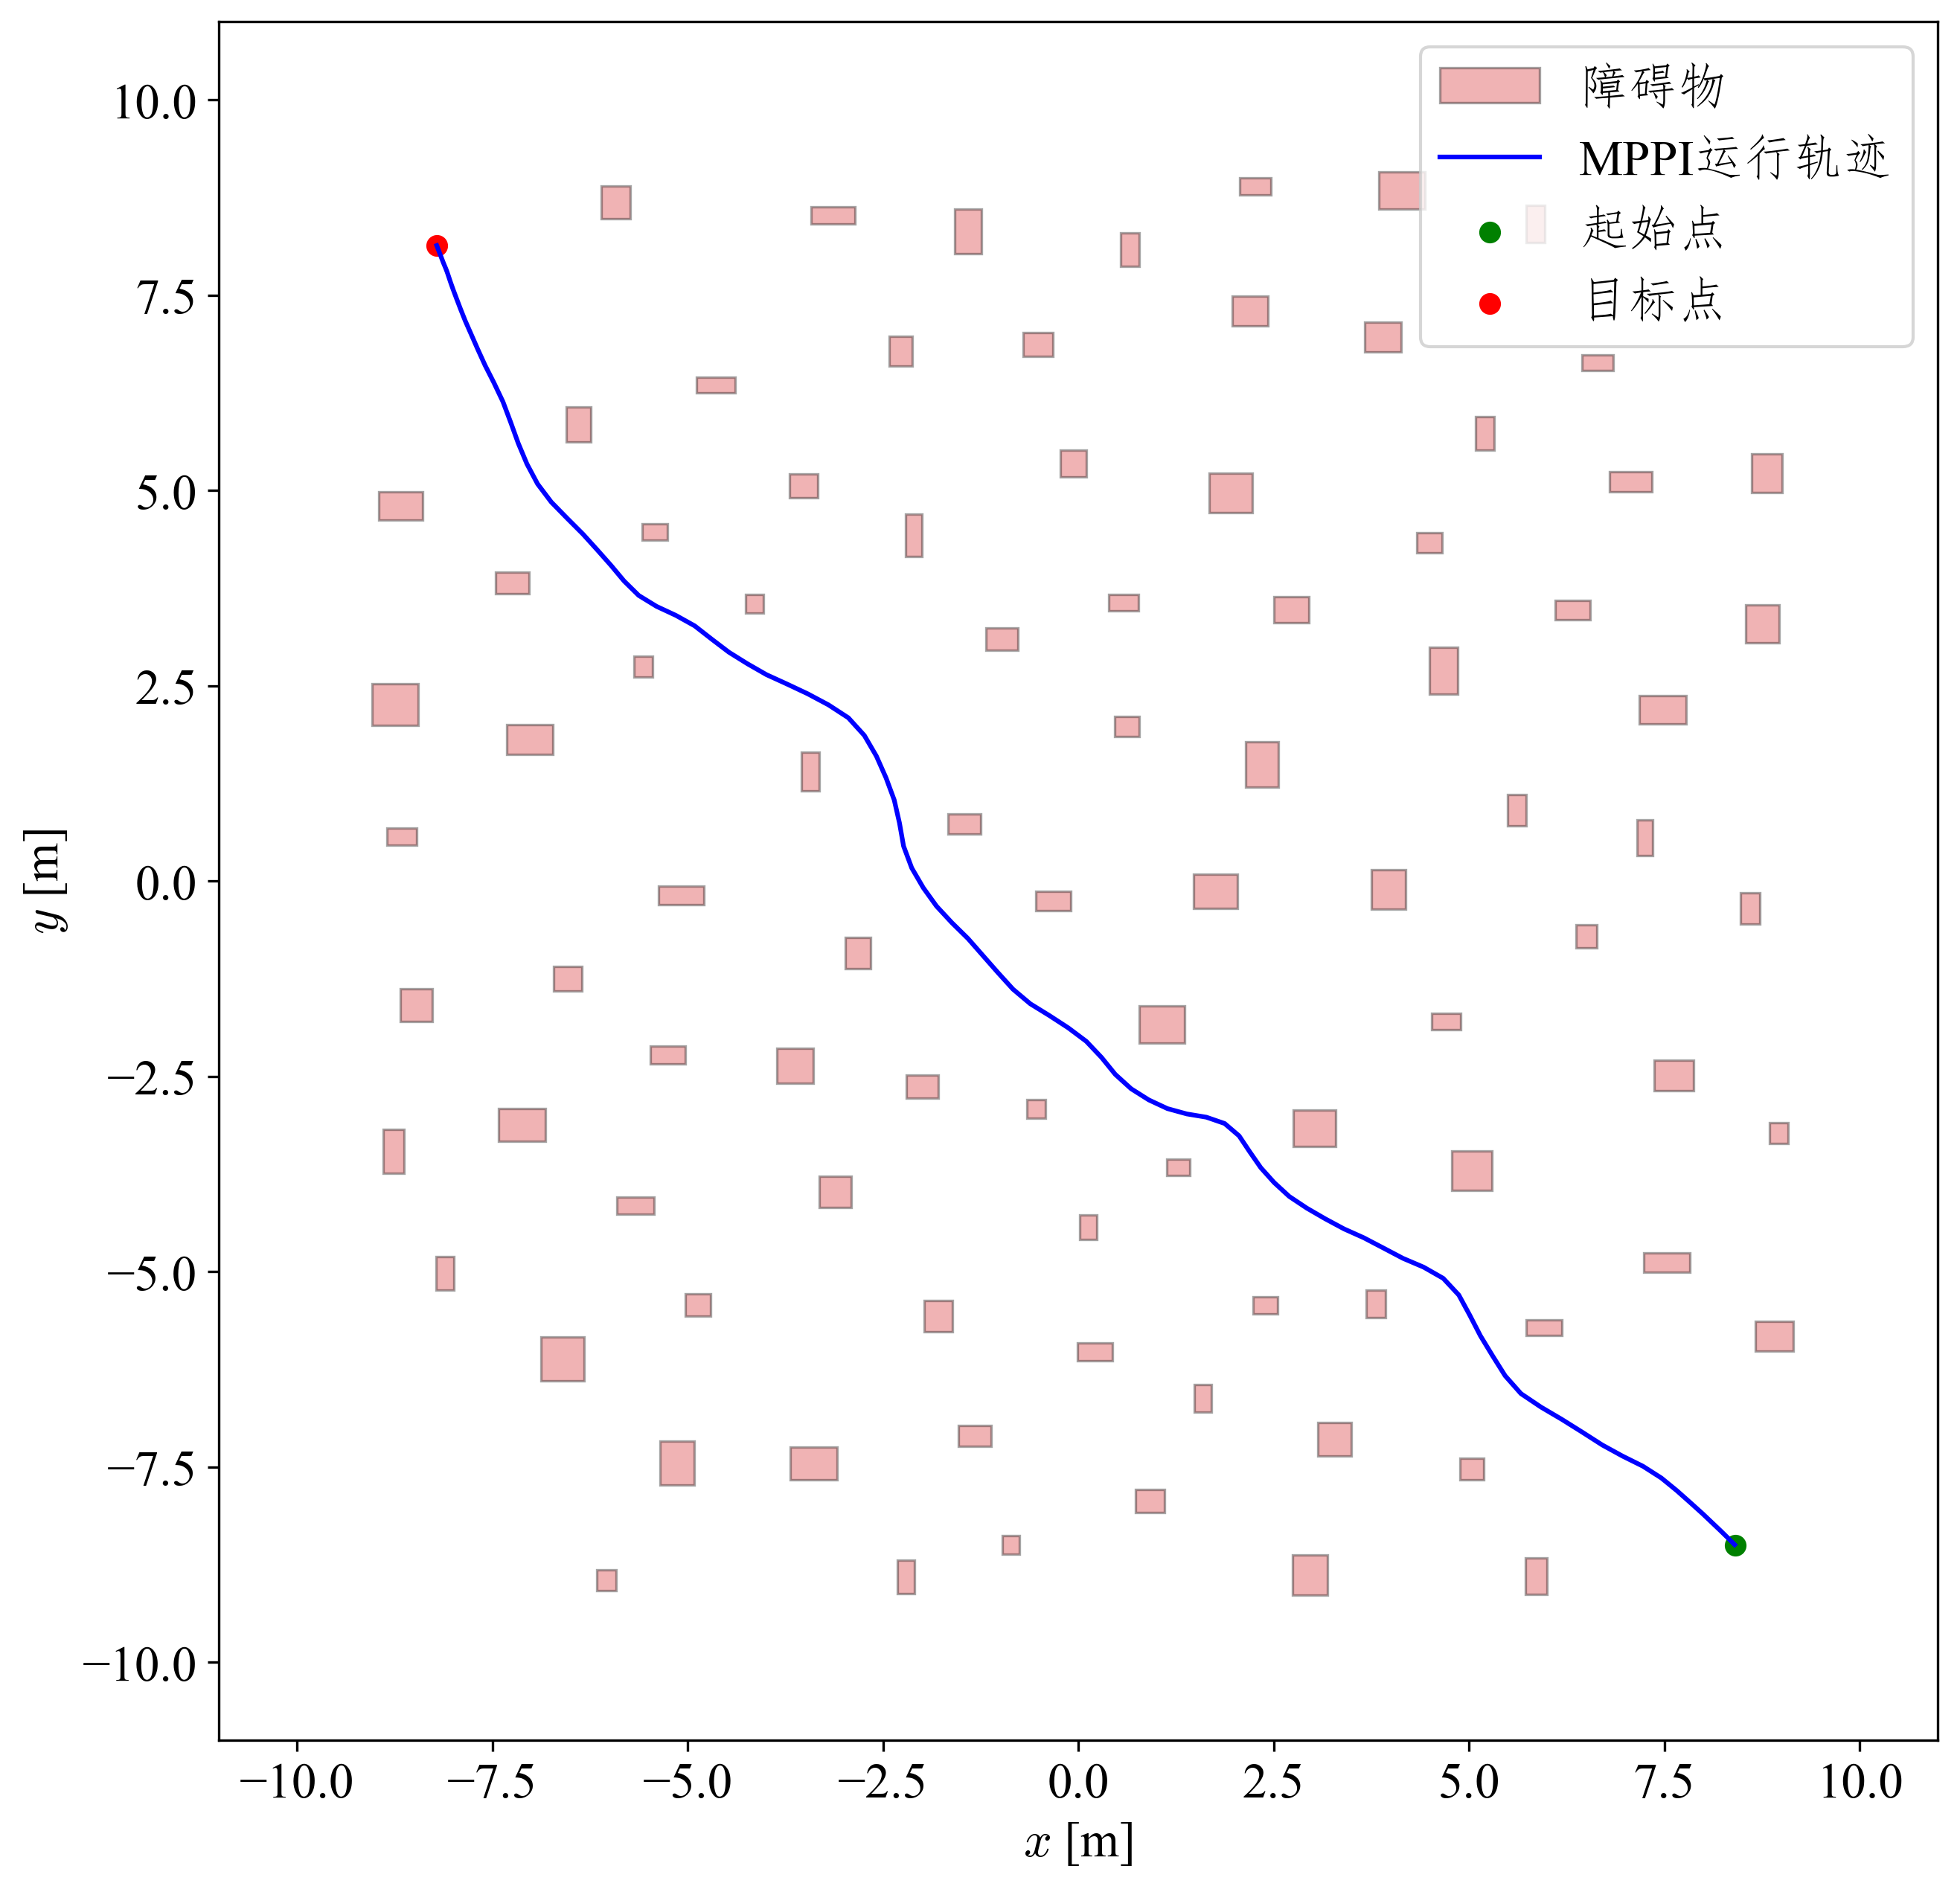
\includegraphics[width=0.33\linewidth]{figure/chapter4/mppi_trajectory_dense_reward.png}}
    \subfloat[无控制平滑的运行轨迹]{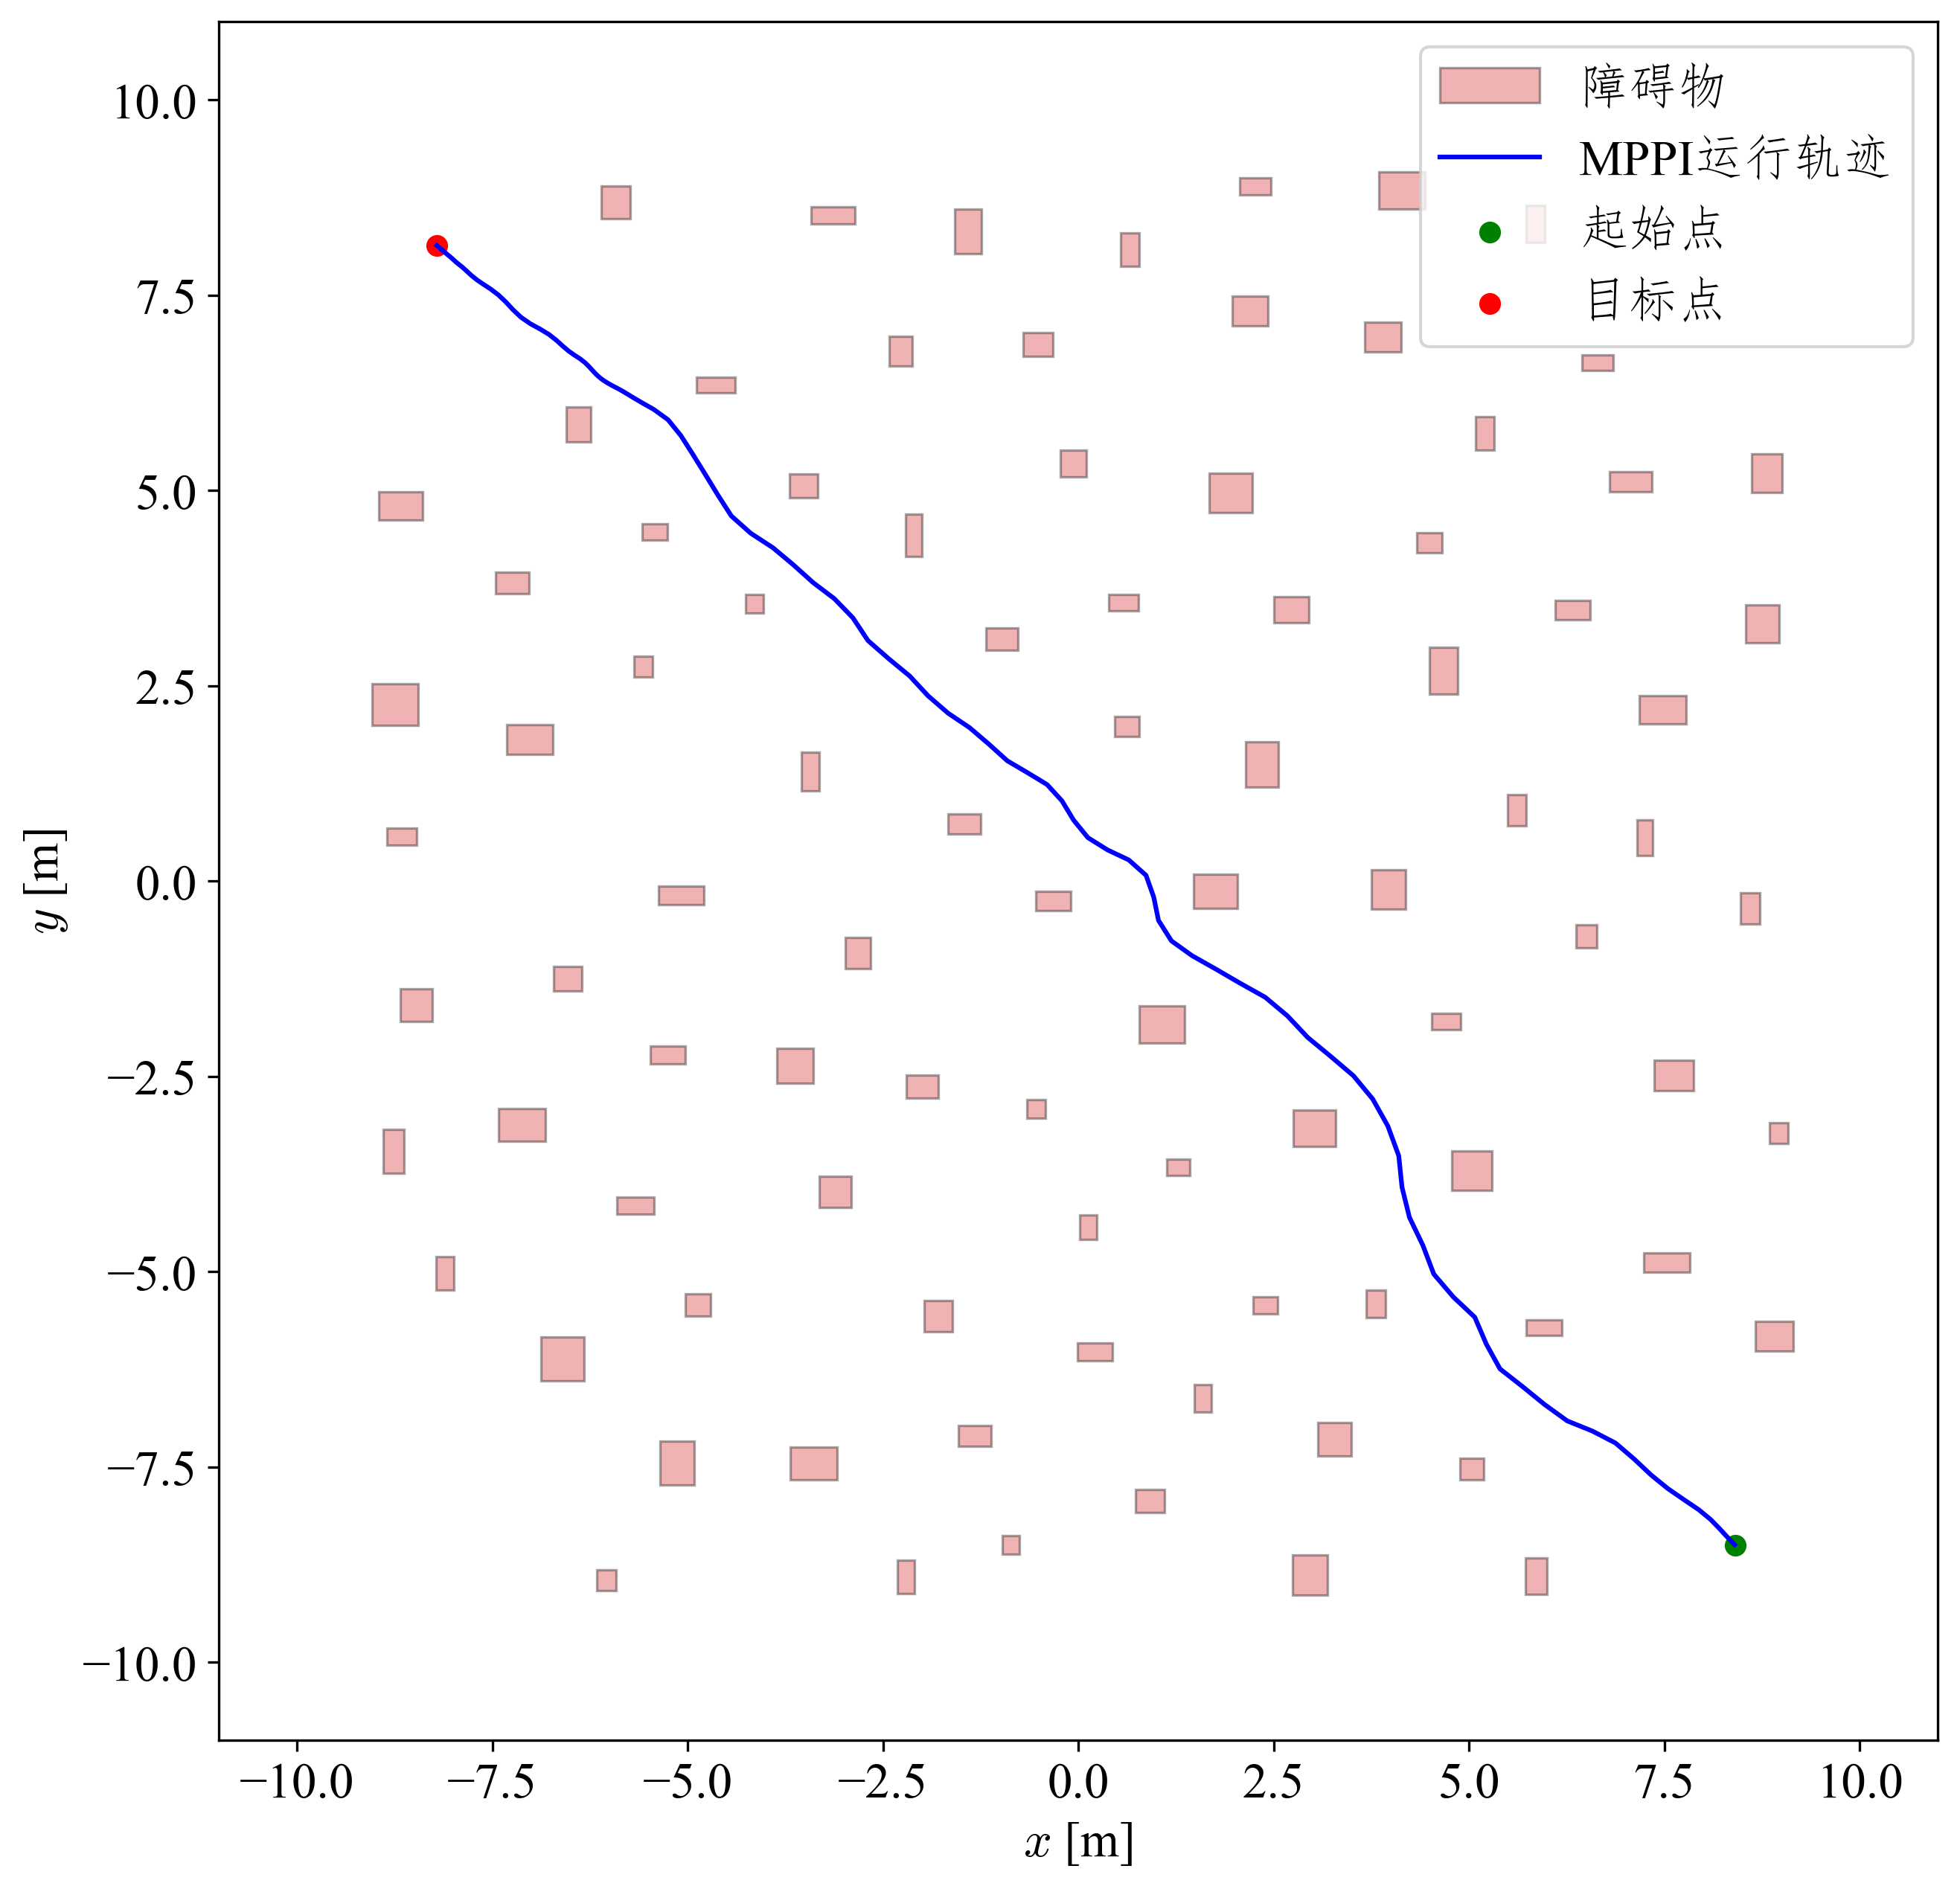
\includegraphics[width=0.33\linewidth]{figure/chapter4/mppi_trajectory_dense_reward_wo_steering.png}}
    \subfloat[无速度惩罚的运行轨迹]{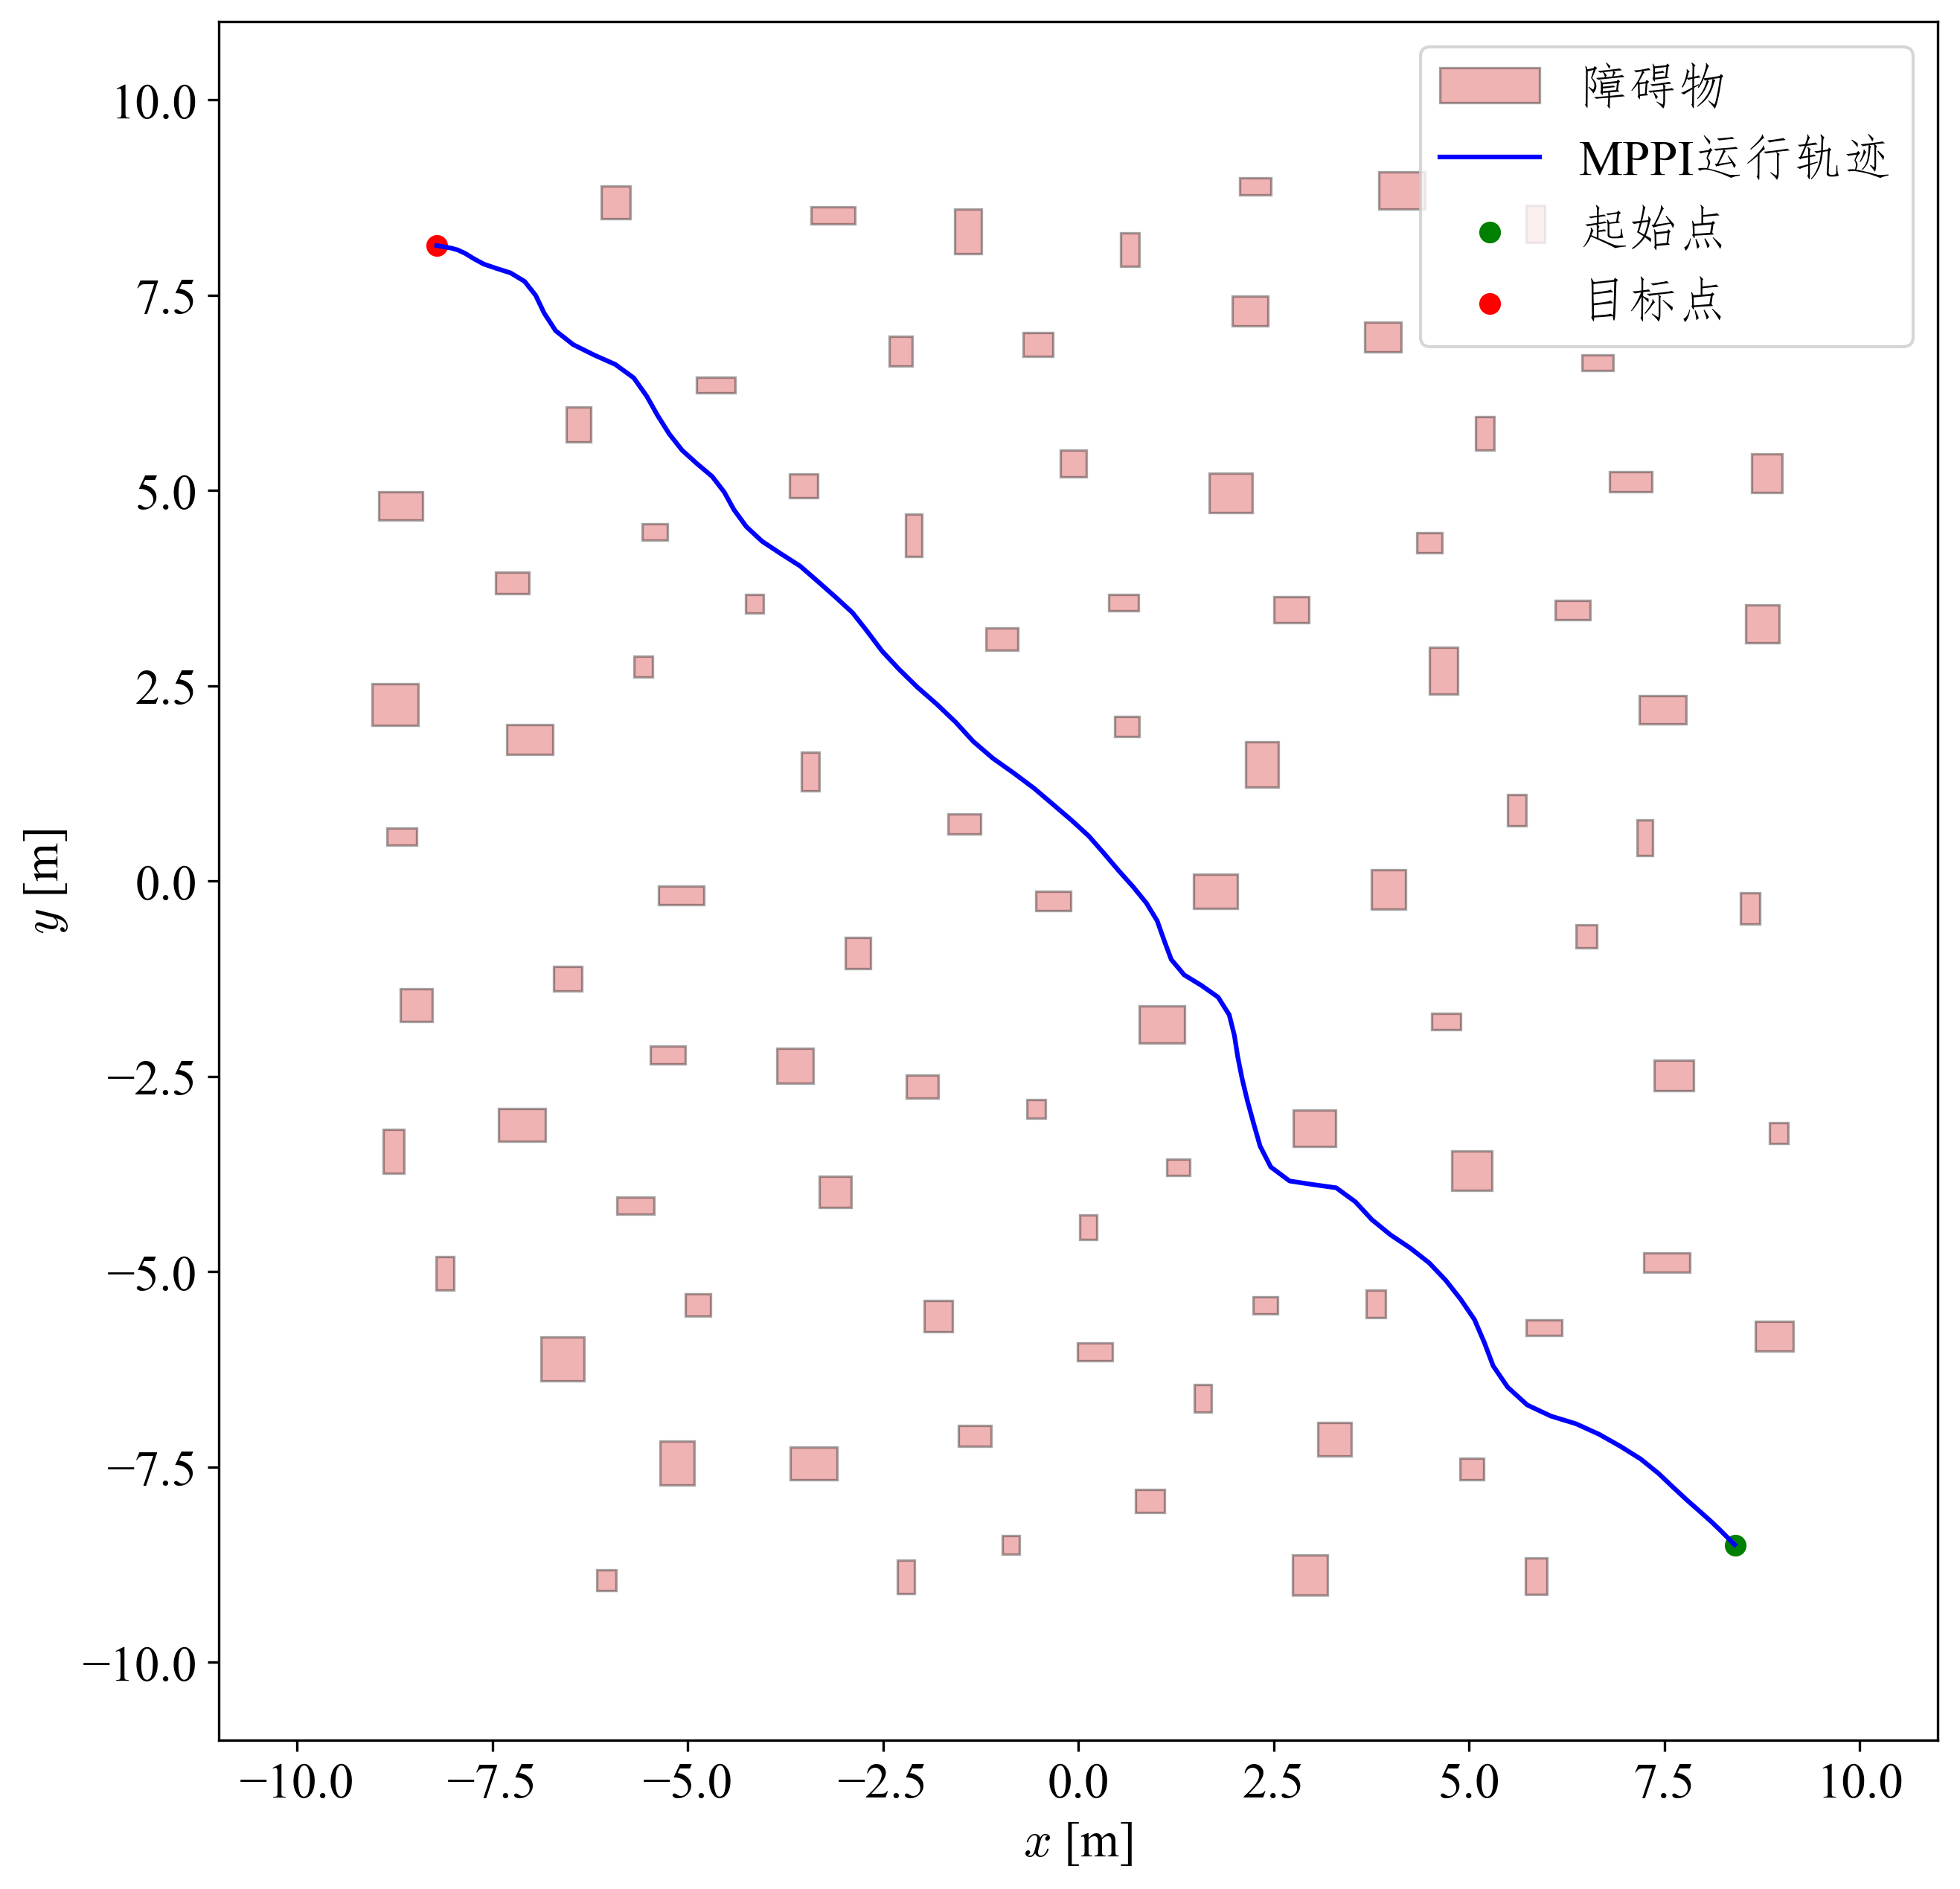
\includegraphics[width=0.33\linewidth]{figure/chapter4/mppi_trajectory_dense_reward_wo_speed.png}}

    \subfloat[本文奖励函数的控制量]{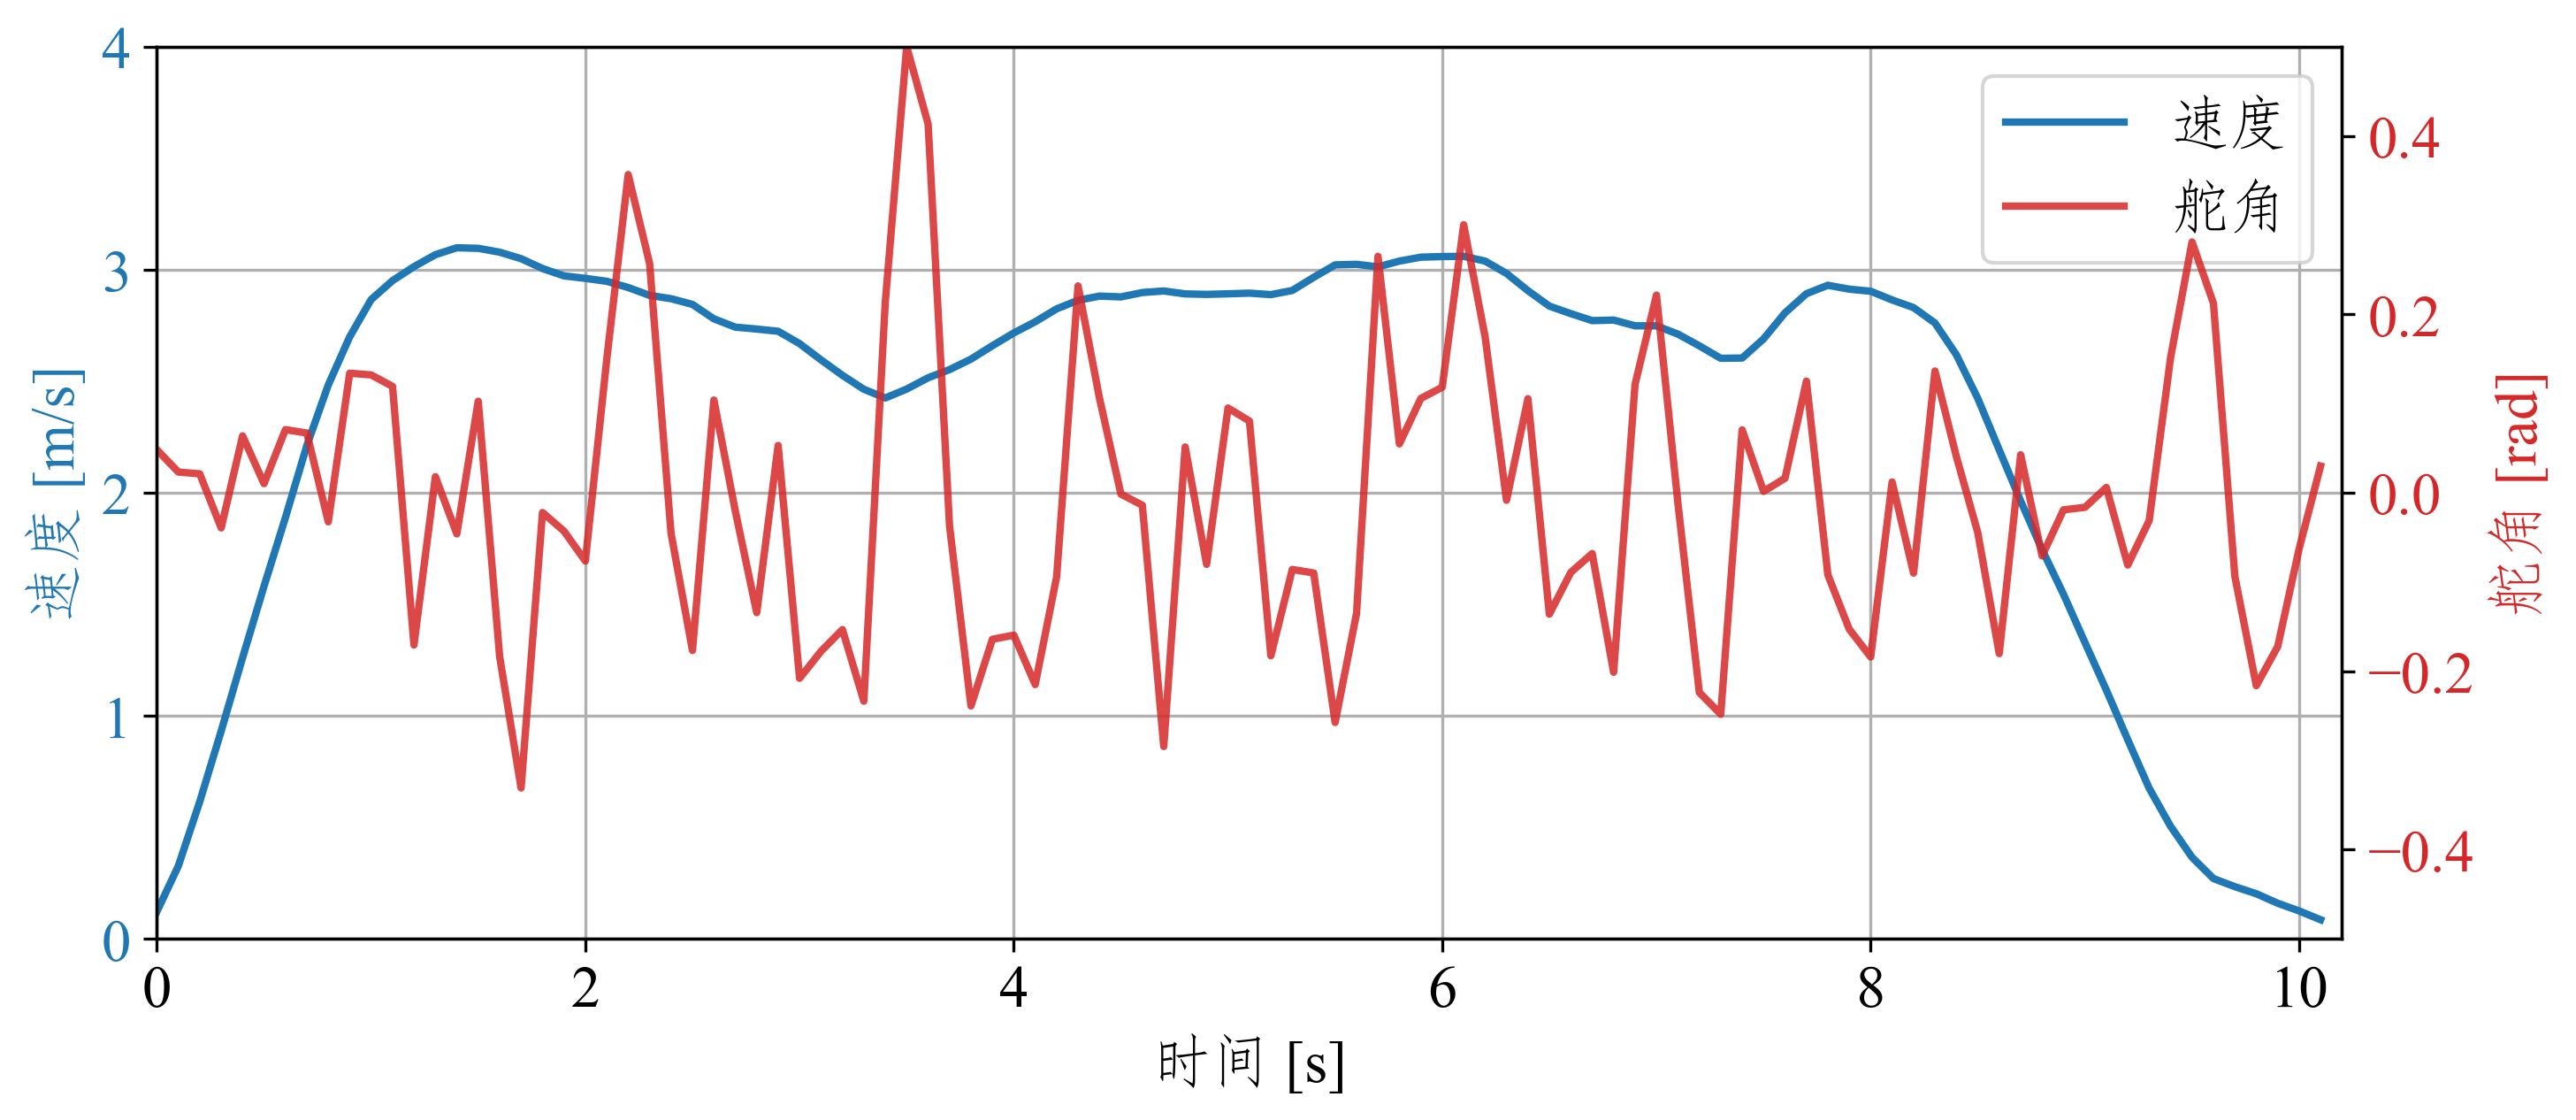
\includegraphics[width=0.33\linewidth]{figure/chapter4/mppi_speed_steering_dense_reward.png}}
    \subfloat[无控制平滑的控制量]{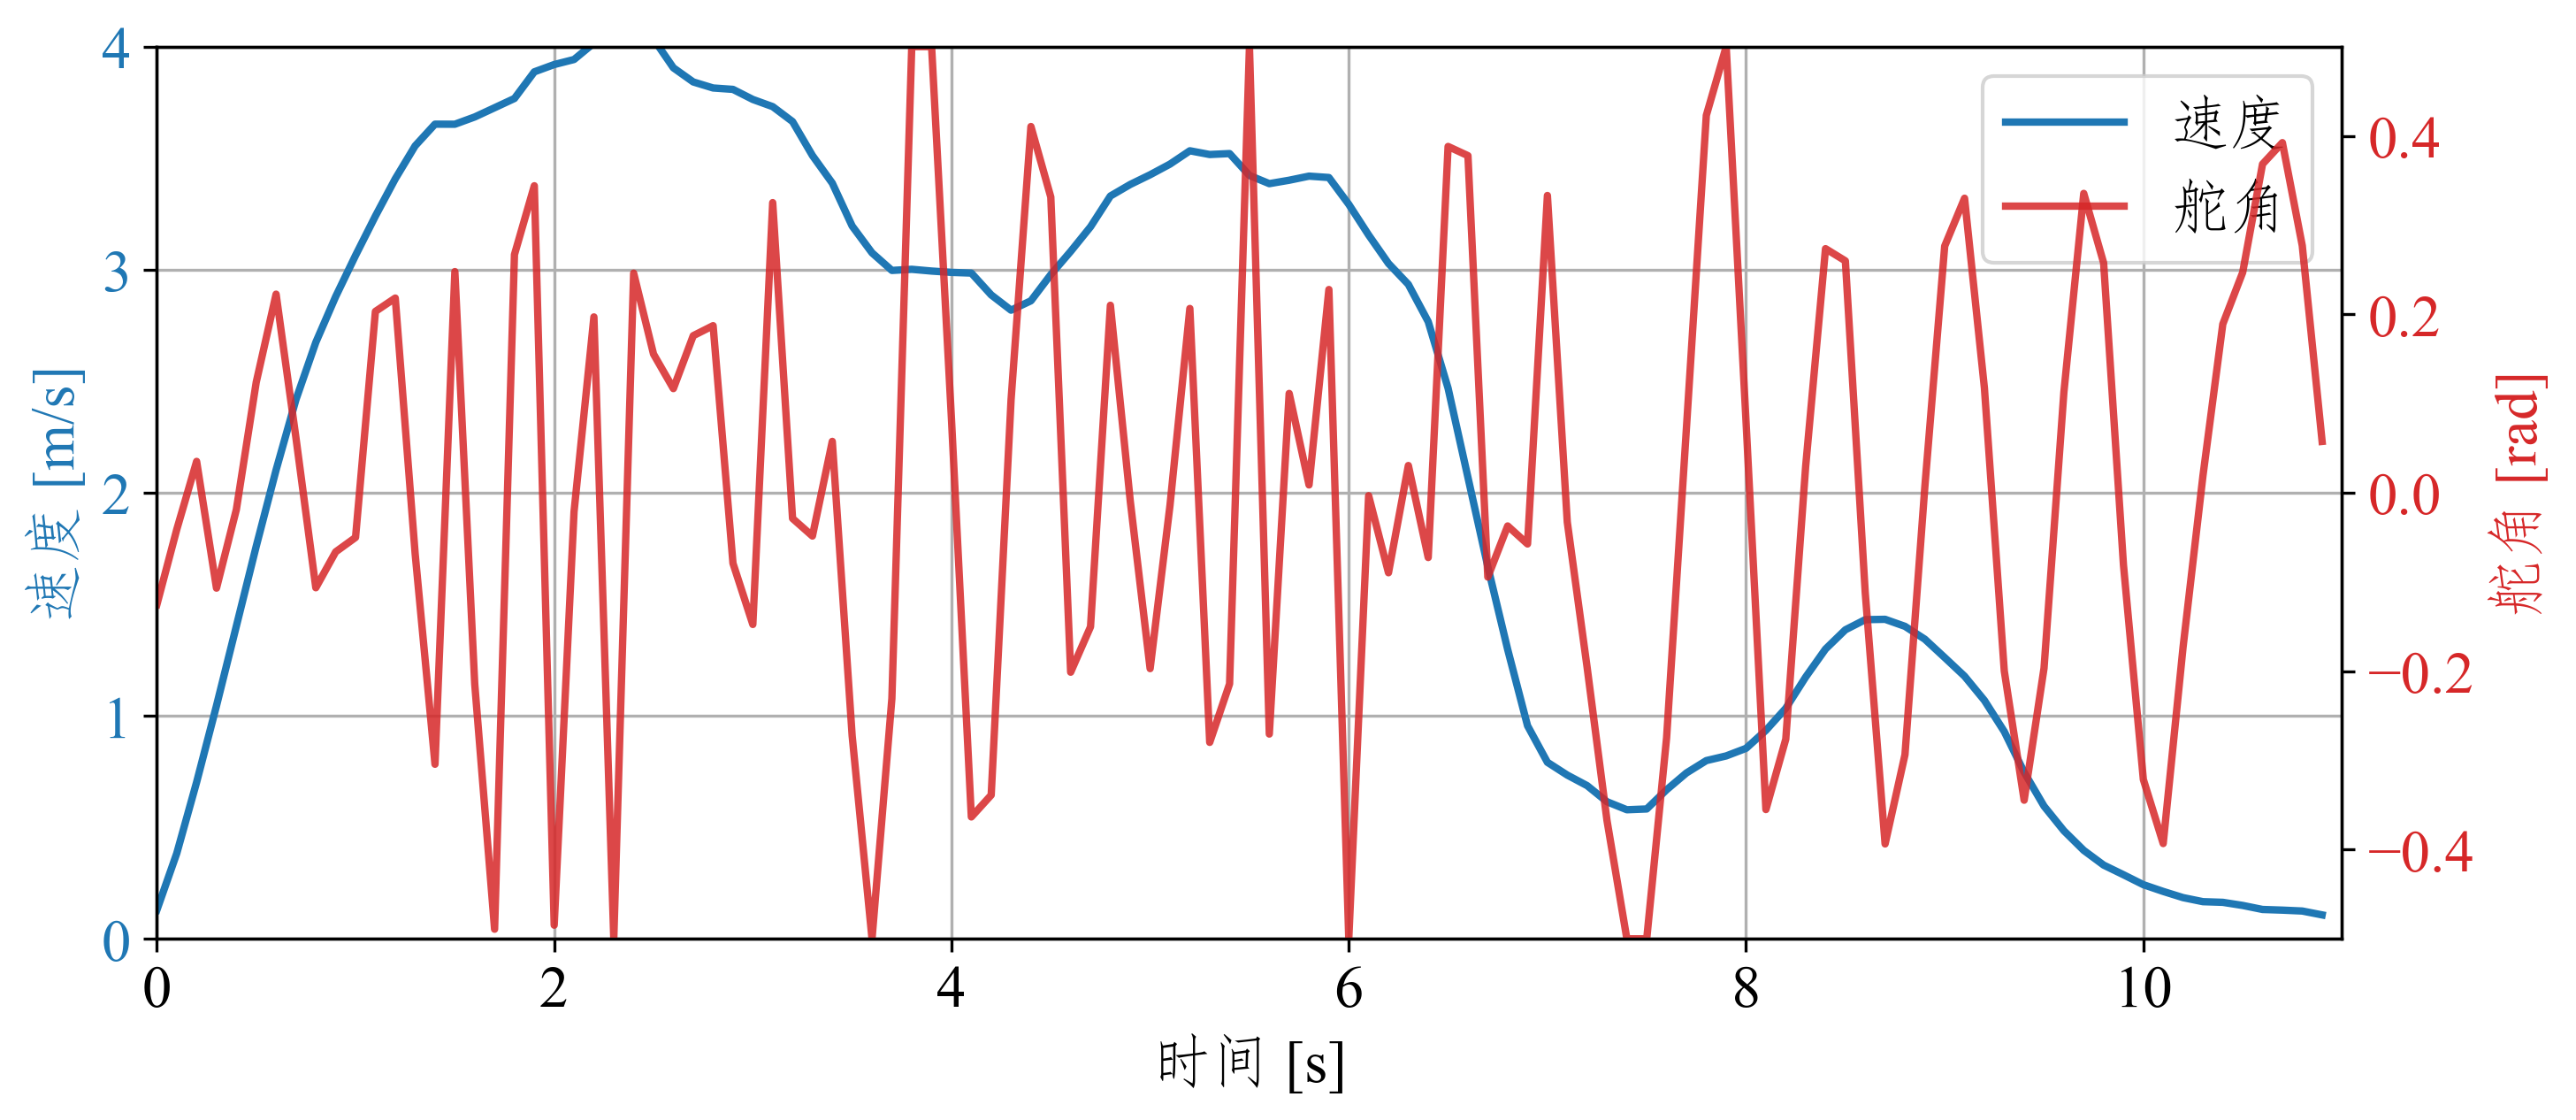
\includegraphics[width=0.33\linewidth]{figure/chapter4/mppi_speed_steering_dense_reward_wo_steering.png}}
    \subfloat[无速度惩罚的控制量]{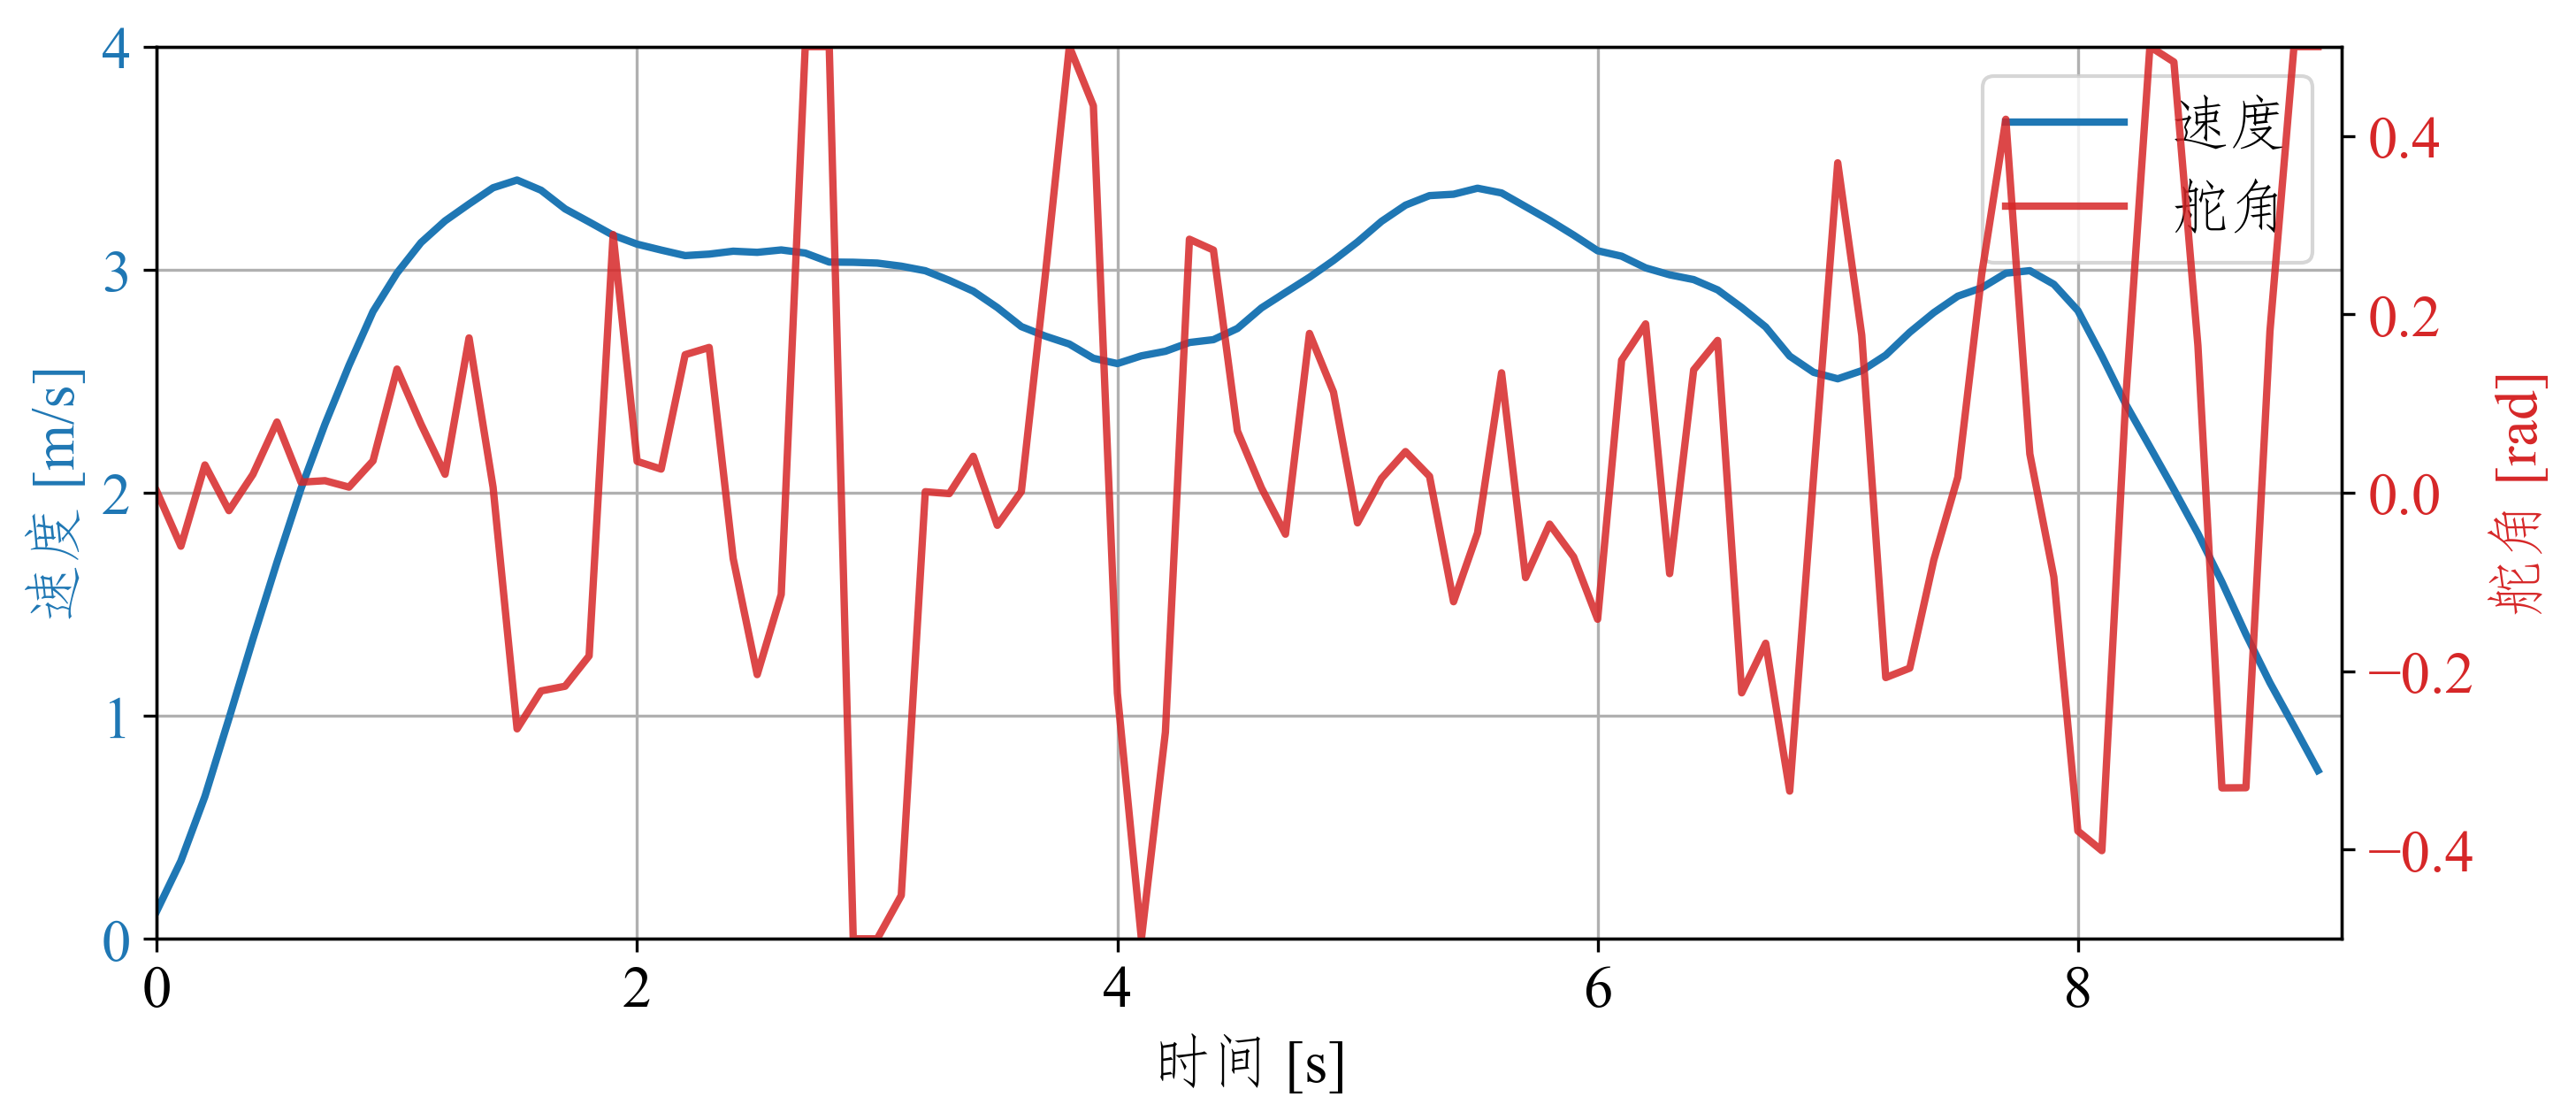
\includegraphics[width=0.33\linewidth]{figure/chapter4/mppi_speed_steering_dense_reward_wo_speed.png}}
    \caption{VPM-MPPI在不同奖励函数下的导航轨迹与控制变化曲线}
    \label{fig:reward-ablation}
\end{figure}
最后，本节还分析了奖励函数设计对导航性能的影响，比较了本文提出的奖励函数与两种简化后的奖励函数：一种是去掉了控制平滑项（\ref{subequ:control-smooth}）的奖励函数，另一种是去掉了速度惩罚项（\ref{subequ:speed-penalty}）的奖励函数。图\ref{fig:reward-ablation}展示了不同奖励函数下的导航轨迹与控制变化曲线。可以看出，本文设计的奖励函数能够生成更平滑、更合理的导航轨迹。去掉控制平滑项后机器人虽然速度更快时间更短，但生成的导航轨迹较为激进，控制输入变化较大；去掉速度惩罚项后机器人在快到达终点时速度不能得到有效控制。结果表明，本文设计的奖励函数能够更好地引导MPPI算法生成平滑、高效的导航控制策略。

\subsection{实车实验}
本节在实车上验证了VPM-MPPI的有效性，硬件组成与第三章相同，实车系统的架构如图\ref{fig:VPM-real-system}所示。VPM在离线阶段使用实车采集的数据进行训练，训练完成后部署在车载计算平台上。在实际导航过程中，MPPI控制器根据VPM的输出生成控制命令，并通过车辆的底层VESC控制器执行。
\begin{figure}[ht]
    \centering
    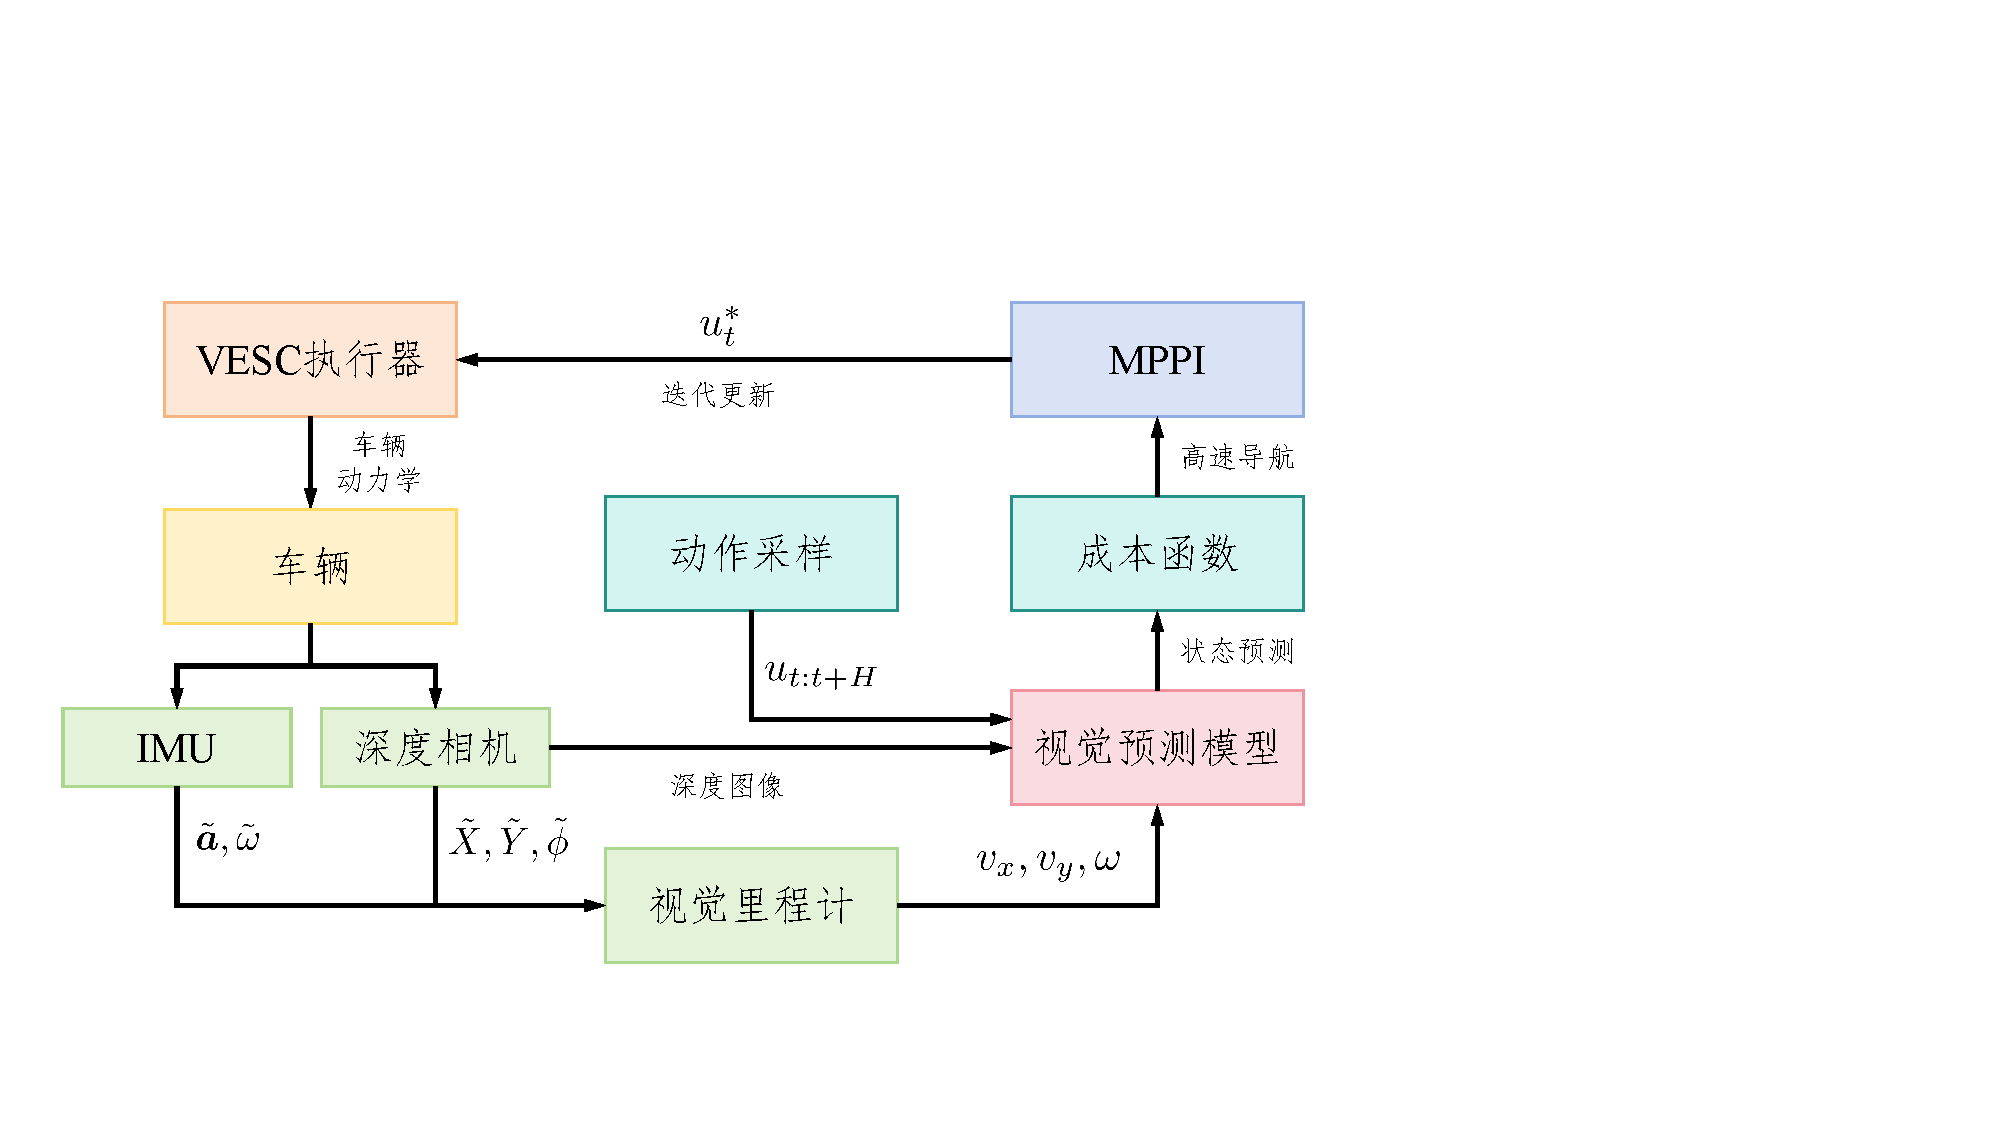
\includegraphics[width=0.6\textwidth]{figure/chapter4/real-system.pdf}
    \caption{VPM-MPPI实车系统架构}
    \label{fig:VPM-real-system}
\end{figure}

实车实验在两个难度不同的地图中进行，分别测试了仿真预训练的VPM和经过2小时实车数据微调后的VPM在实车导航任务中的表现。微调时使用了拥有学习率调整和权重衰减的AdamW优化器，批量大小为128。图\ref{fig:real-experiment}展示了实车实验中的运行轨迹与深度图像，表\ref{table:real-comparison}给出了实车实验中的导航性能比较结果。可以看出，经过实车数据微调后的VPM在两个地图中都实现了100\%的成功率，在平均路径长度和平均到达时间方面也表现出了明显的提升。这些结果表明，VPM-MPPI方法通过实车数据微调可以进一步提升导航性能。

\newpage
\begin{figure}[H]
    \centering
    \subfloat[地图1中的实车运行轨迹]{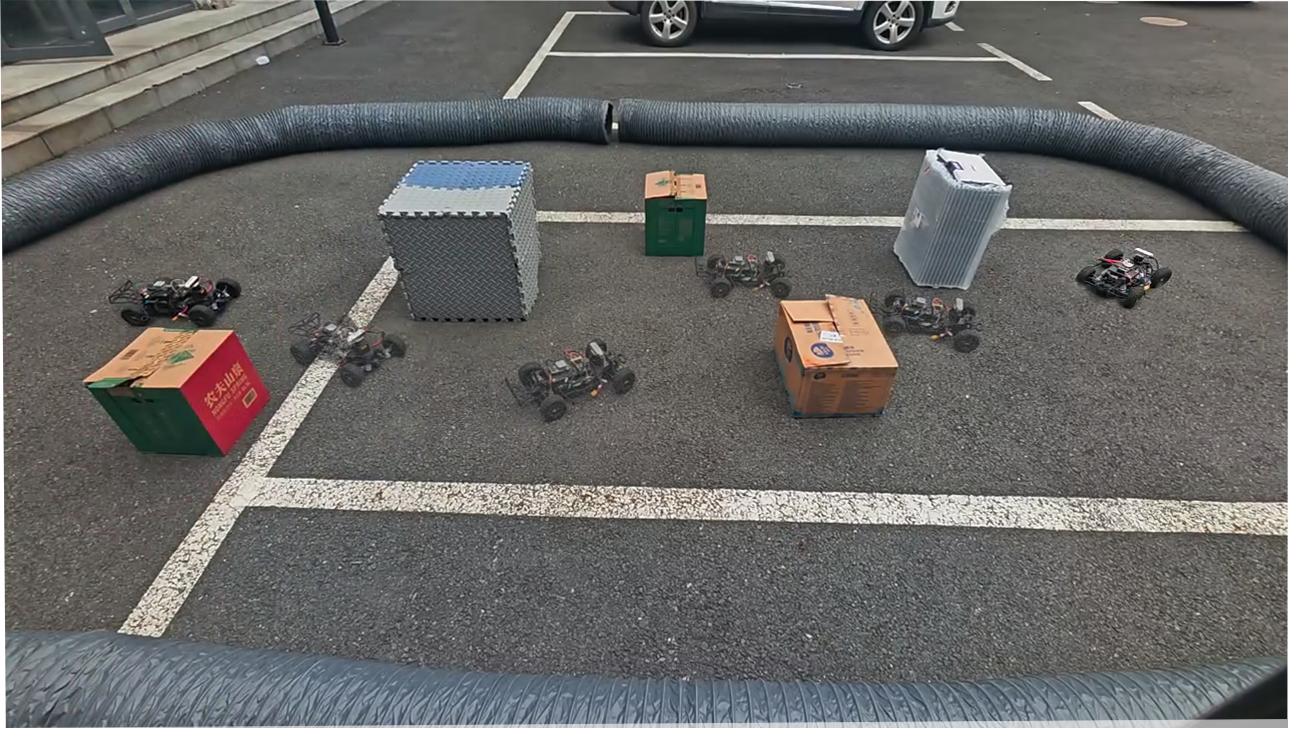
\includegraphics[width=0.5\linewidth]{figure/chapter4/real-map1.png}}

    \subfloat[地图1中的深度图像]{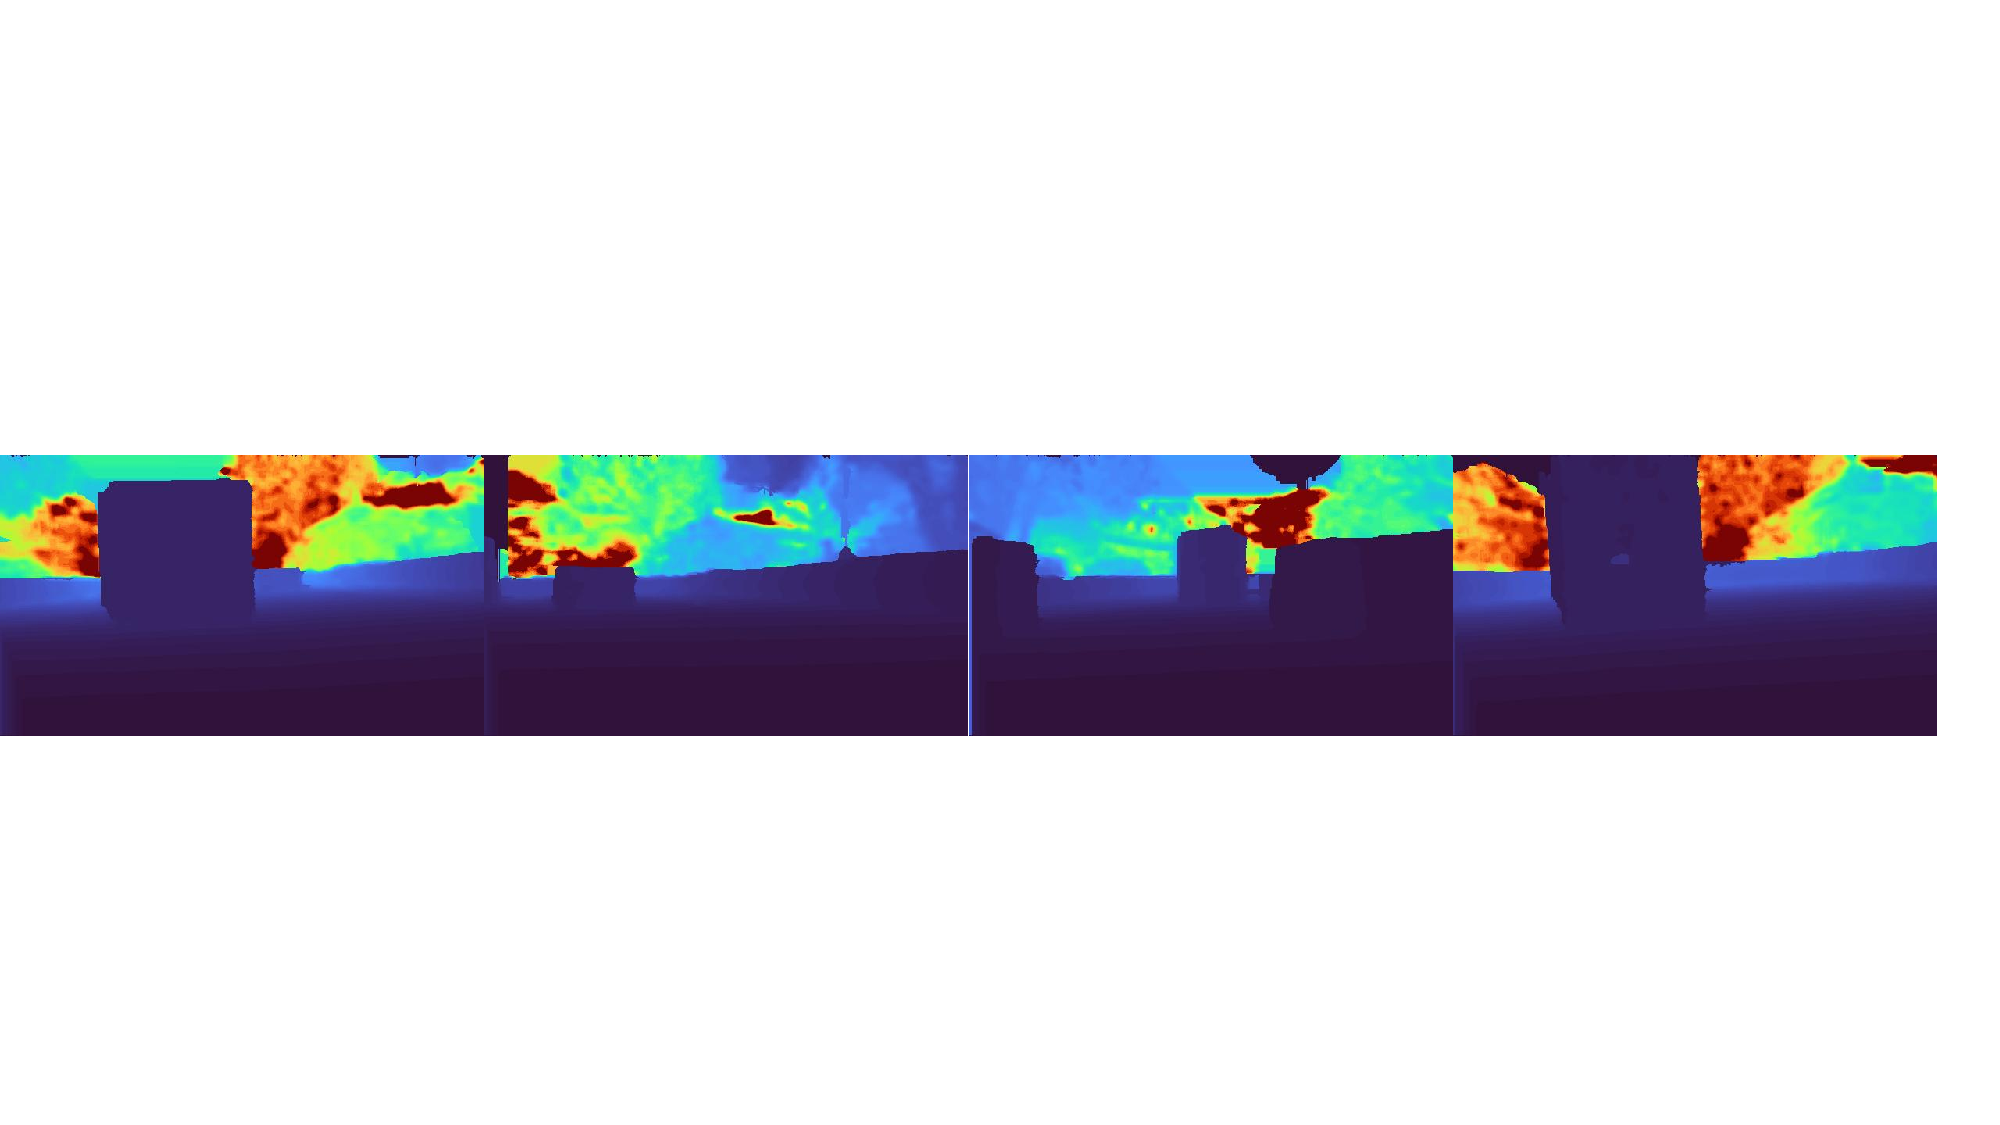
\includegraphics[width=1.0\linewidth]{figure/chapter4/real-depth-1.pdf}}

    \subfloat[地图2中的实车运行轨迹]{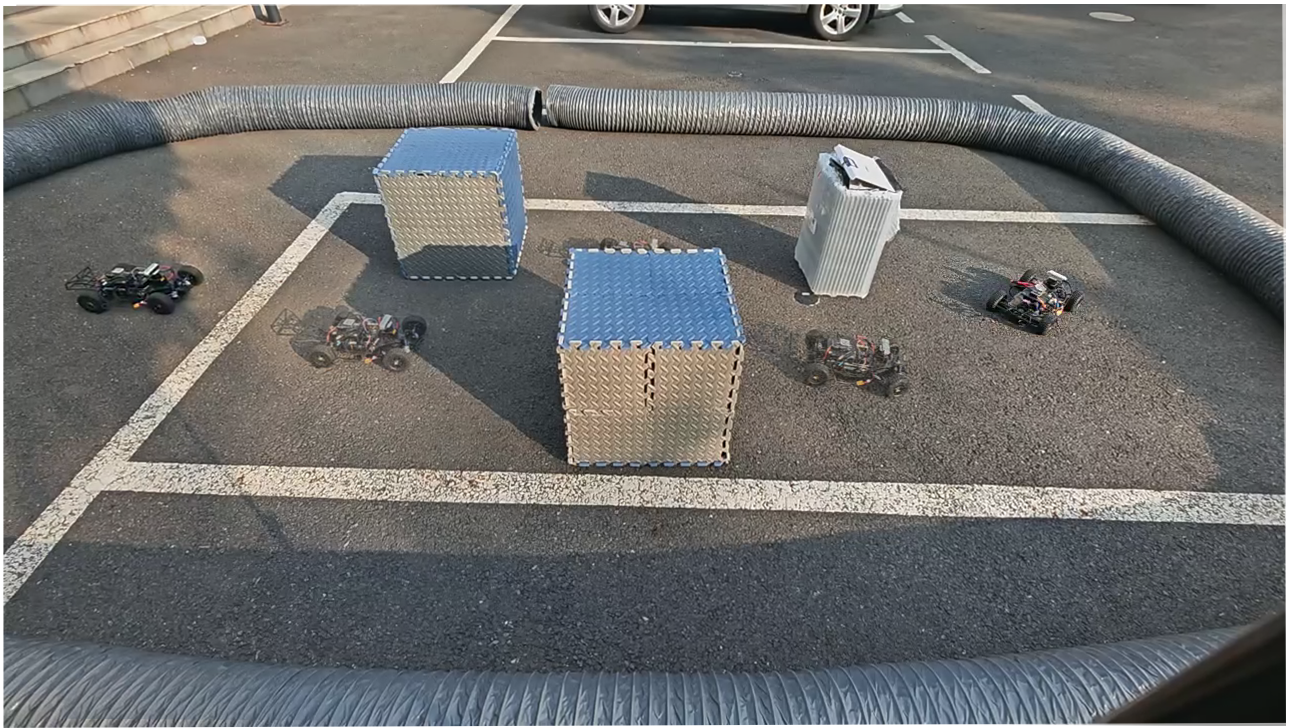
\includegraphics[width=0.5\linewidth]{figure/chapter4/real-map2.png}}

    \subfloat[地图2中的深度图像]{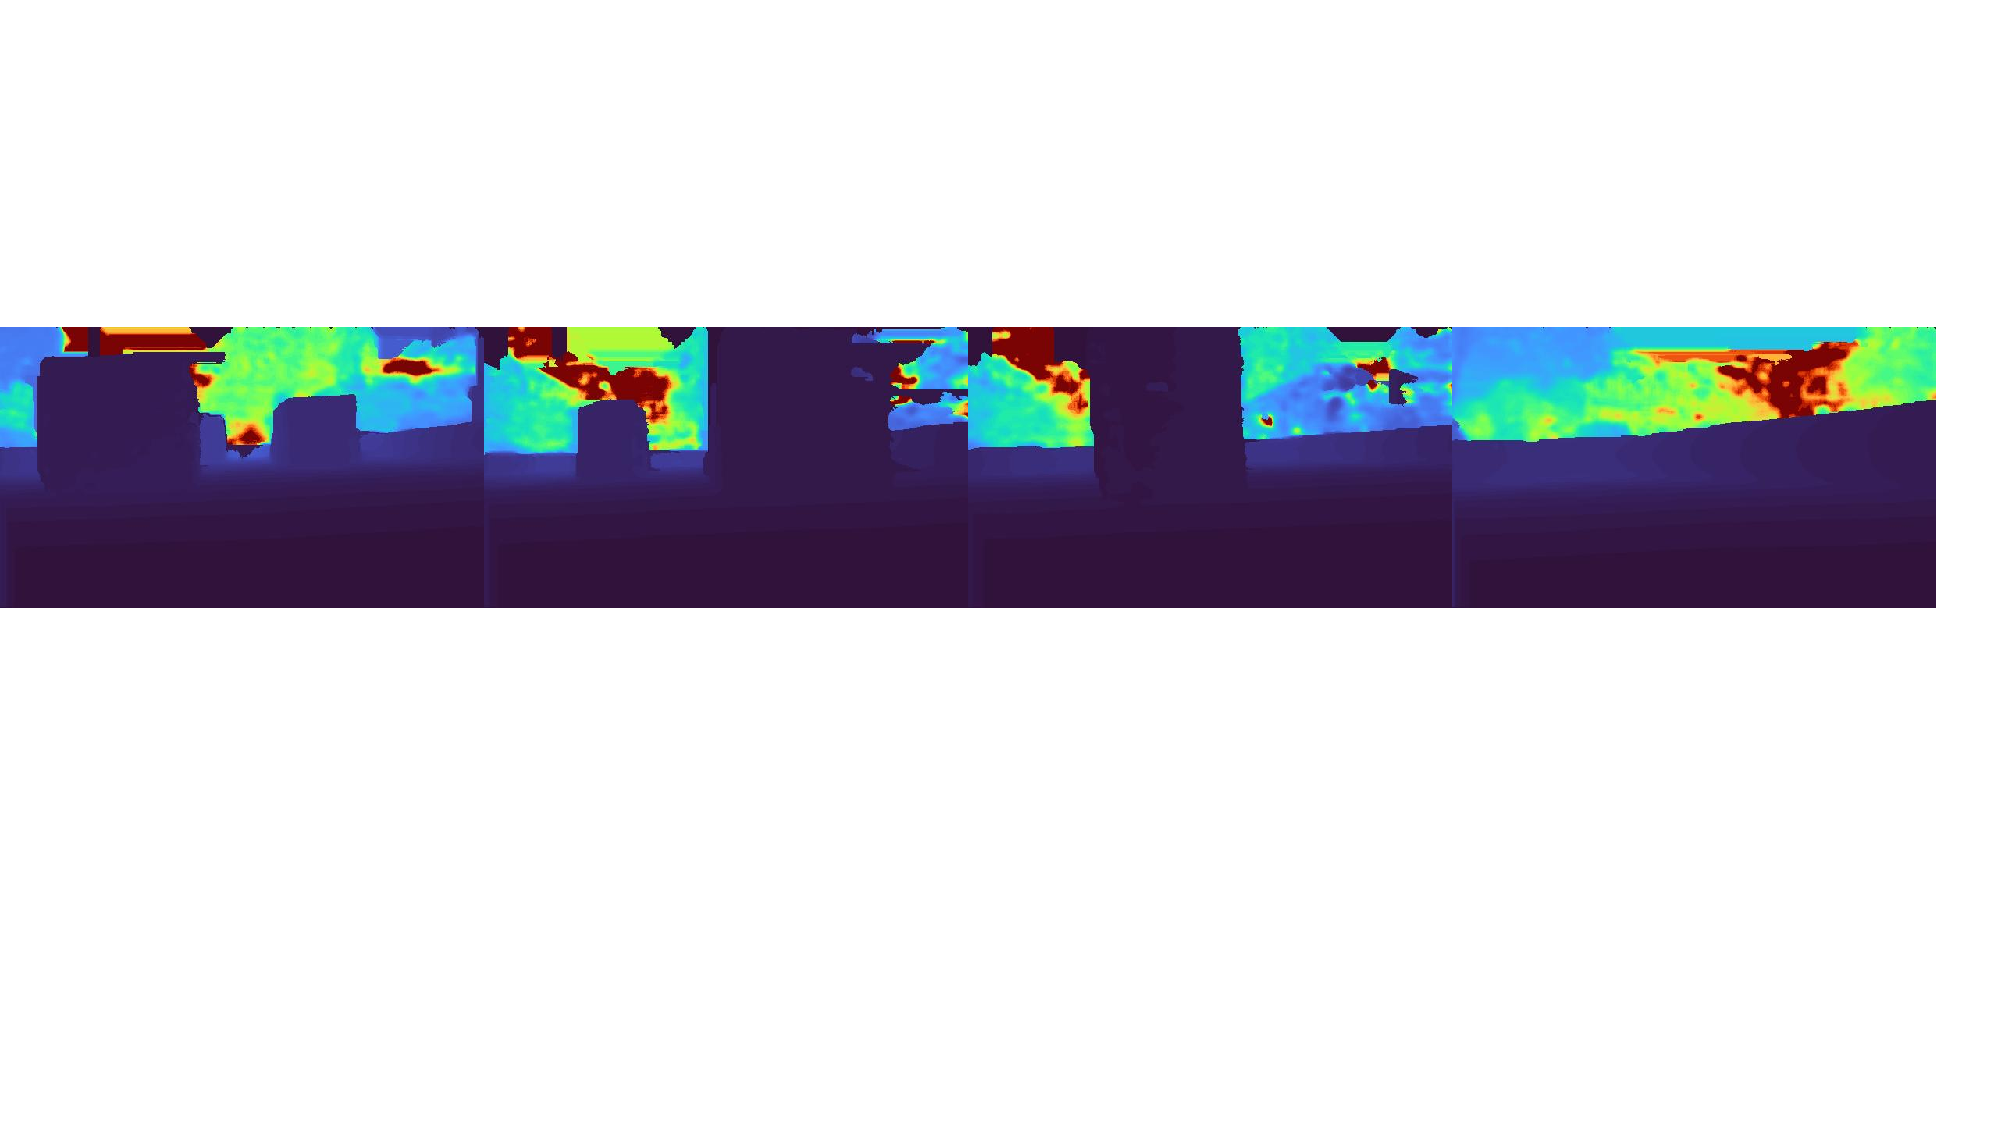
\includegraphics[width=1.0\linewidth]{figure/chapter4/real-depth-2.pdf}}
    \caption{实车实验中的运行轨迹与深度图像}
    \label{fig:real-experiment}
\end{figure}
\begin{table}[H]
\renewcommand{\arraystretch}{1.2}
\caption{实车实验中的导航性能比较}
\centering
\setlength{\tabcolsep}{16pt}{
    \begin{tabular}{ccccc}%四个c代表该表一共四列，内容全部居中
    \toprule[2pt]
    \textbf{地图} & \textbf{模型} & SR[\%] & PL[$m$] & AT[$s$]\\
    \midrule[1pt]
    \multirow{2}{*}{地图1} & 预训练的VPM & $50$ & $7.95\pm0.48$ & $5.93\pm0.27$ \\
    & 微调后的VPM  & $100$ & $7.63\pm0.34$ & $5.29\pm0.19$ \\
    \midrule[1pt]
    \multirow{2}{*}{地图2} & 预训练的VPM & $75$ & $6.99\pm0.41$ & $5.02\pm0.29$\\
    & 微调后的VPM  & $100$ & $6.84\pm0.26$ & $4.79\pm0.21$\\
    \bottomrule[2pt]
\end{tabular}}
\label{table:real-comparison}
\end{table}

\newpage
\section{本章小结}
本章提出了一种基于视觉预测模型的运动控制方法，用于实现高速导航控制。首先，本章介绍了基于循环状态空间模型的视觉预测模型（VPM）的设计与训练方法，使其能够从轨迹数据中学习环境的动力学特征，并提供准确的状态预测。随后，本章将VPM与模型预测路径积分（MPPI）控制算法相结合，设计了一个基于采样的模型预测控制框架，能够利用VPM的预测能力来生成高效的导航控制策略。此外，本章还设计了一个综合考虑目标位置、速度、碰撞和控制平滑性的奖励函数，以引导MPPI算法生成合理的导航轨迹。最后，本章通过仿真和实车实验验证了所提方法在不同环境中的导航性能，并通过消融实验分析了不同设计对导航性能的影响。实验结果表明，基于视觉预测模型的MPPI方法能够实现高速、安全的导航控制，并且通过实车数据微调可以进一步提升导航性能。